% Options for packages loaded elsewhere
\PassOptionsToPackage{unicode}{hyperref}
\PassOptionsToPackage{hyphens}{url}
%
\documentclass[
]{book}
\usepackage{amsmath,amssymb}
\usepackage{iftex}
\ifPDFTeX
  \usepackage[T1]{fontenc}
  \usepackage[utf8]{inputenc}
  \usepackage{textcomp} % provide euro and other symbols
\else % if luatex or xetex
  \usepackage{unicode-math} % this also loads fontspec
  \defaultfontfeatures{Scale=MatchLowercase}
  \defaultfontfeatures[\rmfamily]{Ligatures=TeX,Scale=1}
\fi
\usepackage{lmodern}
\ifPDFTeX\else
  % xetex/luatex font selection
\fi
% Use upquote if available, for straight quotes in verbatim environments
\IfFileExists{upquote.sty}{\usepackage{upquote}}{}
\IfFileExists{microtype.sty}{% use microtype if available
  \usepackage[]{microtype}
  \UseMicrotypeSet[protrusion]{basicmath} % disable protrusion for tt fonts
}{}
\makeatletter
\@ifundefined{KOMAClassName}{% if non-KOMA class
  \IfFileExists{parskip.sty}{%
    \usepackage{parskip}
  }{% else
    \setlength{\parindent}{0pt}
    \setlength{\parskip}{6pt plus 2pt minus 1pt}}
}{% if KOMA class
  \KOMAoptions{parskip=half}}
\makeatother
\usepackage{xcolor}
\usepackage{longtable,booktabs,array}
\usepackage{calc} % for calculating minipage widths
% Correct order of tables after \paragraph or \subparagraph
\usepackage{etoolbox}
\makeatletter
\patchcmd\longtable{\par}{\if@noskipsec\mbox{}\fi\par}{}{}
\makeatother
% Allow footnotes in longtable head/foot
\IfFileExists{footnotehyper.sty}{\usepackage{footnotehyper}}{\usepackage{footnote}}
\makesavenoteenv{longtable}
\usepackage{graphicx}
\makeatletter
\def\maxwidth{\ifdim\Gin@nat@width>\linewidth\linewidth\else\Gin@nat@width\fi}
\def\maxheight{\ifdim\Gin@nat@height>\textheight\textheight\else\Gin@nat@height\fi}
\makeatother
% Scale images if necessary, so that they will not overflow the page
% margins by default, and it is still possible to overwrite the defaults
% using explicit options in \includegraphics[width, height, ...]{}
\setkeys{Gin}{width=\maxwidth,height=\maxheight,keepaspectratio}
% Set default figure placement to htbp
\makeatletter
\def\fps@figure{htbp}
\makeatother
\setlength{\emergencystretch}{3em} % prevent overfull lines
\providecommand{\tightlist}{%
  \setlength{\itemsep}{0pt}\setlength{\parskip}{0pt}}
\setcounter{secnumdepth}{5}
\usepackage{booktabs}
\ifLuaTeX
  \usepackage{selnolig}  % disable illegal ligatures
\fi
\usepackage[]{natbib}
\bibliographystyle{apalike}
\IfFileExists{bookmark.sty}{\usepackage{bookmark}}{\usepackage{hyperref}}
\IfFileExists{xurl.sty}{\usepackage{xurl}}{} % add URL line breaks if available
\urlstyle{same}
\hypersetup{
  pdftitle={Social Media Analytics},
  pdfauthor={AP Leith},
  hidelinks,
  pdfcreator={LaTeX via pandoc}}

\title{Social Media Analytics}
\usepackage{etoolbox}
\makeatletter
\providecommand{\subtitle}[1]{% add subtitle to \maketitle
  \apptocmd{\@title}{\par {\large #1 \par}}{}{}
}
\makeatother
\subtitle{An R Guide for Media Researchers}
\author{AP Leith\footnote{Southern Illinois University Edwardsville, \href{mailto:aleith@siue.edu}{\nolinkurl{aleith@siue.edu}}}}
\date{2024-02-06}

\begin{document}
\maketitle

{
\setcounter{tocdepth}{1}
\tableofcontents
}
\hypertarget{preface}{%
\chapter*{Preface}\label{preface}}
\addcontentsline{toc}{chapter}{Preface}

Welcome to ``Social Media Analytics: An R Guide for Media Researchers,'' a comprehensive guide designed to navigate the intricate pathways of social media analytics in the ever-evolving field of mass communications. This textbook is a culmination of my journey in academia and a reflection of my commitment to advancing the understanding of social media analytics, particularly through the lens of quantitative analysis using R and RStudio.

This book heavily leans on American-dominant social network sites in its discussions on social media. This will not be permanent as future iterations of this text will expand to include more global examples tha include social media beyond social networking sites.

I am Dr.~Alex P. Leith, currently serving as an Assistant Professor in the Department of Mass Communications at Southern Illinois University Edwardsville. My academic journey, which began with a Ph.D.~in Information and Media from Michigan State University, has been a blend of rigorous research and practical application in the fields of digital media, virtual reality, and the social dimensions of digital media. My dissertation, ``Gameplay Livestreaming: Agents of Gamespace,'' set the stage for my ongoing exploration of contemporary digital media trends.

My professional trajectory has been diverse, encompassing roles as a Graduate Assistant at Michigan State University, an Adjunct Instructor at McKendree University and St.~Louis College of Pharmacy, and a Marketing Manager at Brigham Young University -- Idaho. These experiences have enriched my understanding of the multifaceted nature of mass communications, both in academic and practical contexts.

This textbook is a unique endeavor, coalesced with the assistance of ChatGPT 4, a state-of-the-art language model developed by OpenAI. The collaboration with ChatGPT 4 has enabled the integration of advanced AI insights into the book's development, ensuring a blend of human expertise and technological innovation.

``Quantitative Research in Mass Communications'' is structured to guide readers from the foundational aspects of mass communication research and ethics, through the complexities of IRB certification, to the development of research interests and the intricacies of conducting literature reviews. It further delves into the practicalities of formulating research questions, designing quantitative studies, and harnessing the power of R and RStudio for data management, analysis, and visualization. The book culminates with insights into engaging public audiences, writing for them, and presenting research findings effectively.

My research, reflected in publications like ``Psychology of Popular Media'' and ``IEEE Transactions on Games,'' and my success in securing funding for research projects have significantly influenced the content of this textbook. The book aims not only to impart knowledge but also to inspire innovation and critical thinking in the field of mass communications.

As readers embark on this journey through ``Quantitative Research in Mass Communications,'' my hope is that this textbook serves as a valuable resource, aiding in the development of skilled, insightful, and ethically grounded researchers in the dynamic realm of mass communications.

Dr.~Alex P. Leith
Assistant Professor
Department of Mass Communications
Southern Illinois University Edwardsville

\hypertarget{introduction-to-social-media-types}{%
\chapter{Introduction to Social Media Types}\label{introduction-to-social-media-types}}

\hypertarget{overview-of-different-social-media-platforms}{%
\section*{Overview of Different Social Media Platforms}\label{overview-of-different-social-media-platforms}}
\addcontentsline{toc}{section}{Overview of Different Social Media Platforms}

Social media has evolved into a complex ecosystem, each platform with its unique culture, demographic, and influence. Understanding these platforms' characteristics is crucial for navigating the social media landscape effectively, whether for personal use, marketing, or research. This section provides an overview of various social media platforms, their comparative features, historical evolution, cultural nuances, and their broader impact on media and communication.

\hypertarget{introduction}{%
\subsection*{Introduction}\label{introduction}}
\addcontentsline{toc}{subsection}{Introduction}

\begin{itemize}
\tightlist
\item
  \textbf{Defining Social Media}: The section begins by defining social media as digital platforms that facilitate the creation, sharing, and exchange of content, ideas, career interests, and other forms of expression via virtual communities and networks.
\item
  \textbf{Role in Contemporary Society}: It would highlight social media's role in today's society, touching upon its impact on communication, information dissemination, networking, and entertainment.
\end{itemize}

\hypertarget{comparative-analysis-of-platforms}{%
\subsection*{Comparative Analysis of Platforms}\label{comparative-analysis-of-platforms}}
\addcontentsline{toc}{subsection}{Comparative Analysis of Platforms}

\begin{itemize}
\tightlist
\item
  \textbf{Facebook}: As one of the oldest and most diverse platforms, Facebook is characterized by its broad user base and features that cater to personal networking, business promotion, entertainment, and news dissemination.
\item
  \textbf{Twitter}: Known for its brevity and immediacy, Twitter serves as a platform for real-time updates, public discourse, and a significant channel for news and political commentary.
\item
  \textbf{Instagram}: Focused on visual content, Instagram is popular for its photo and video sharing capabilities, appealing largely to a younger demographic seeking creative expression and lifestyle inspiration.
\item
  \textbf{LinkedIn}: This platform stands out for its professional networking focus, connecting individuals and organizations for career-related purposes, industry discussions, and corporate branding.
\item
  \textbf{TikTok}: A newer entrant, TikTok has rapidly gained popularity for its short-form video content, appealing particularly to Gen Z users with its entertainment-focused and interactive content.
\end{itemize}

\hypertarget{historical-context}{%
\subsection*{Historical Context}\label{historical-context}}
\addcontentsline{toc}{subsection}{Historical Context}

\begin{itemize}
\tightlist
\item
  \textbf{Evolution of Platforms}: The section would trace the evolution of these platforms, noting key developmental milestones such as Facebook's expansion from a college network to a global platform, Twitter's role in social movements, and LinkedIn's progression in professional networking.
\item
  \textbf{Technological Advancements}: The role of technological advancements in shaping these platforms, such as the integration of AI in content curation and the rise of mobile computing influencing platform accessibility and user experience.
\end{itemize}

\hypertarget{platform-specific-culture-and-etiquette}{%
\subsection*{Platform-Specific Culture and Etiquette}\label{platform-specific-culture-and-etiquette}}
\addcontentsline{toc}{subsection}{Platform-Specific Culture and Etiquette}

\begin{itemize}
\tightlist
\item
  \textbf{Cultural Nuances}: Each platform's unique cultural nuances, like Twitter's hashtag culture facilitating global conversations, Instagram's emphasis on aesthetics, and LinkedIn's formal and professional tone.
\item
  \textbf{Etiquette and Best Practices}: Discussing the unwritten rules and etiquette specific to each platform, such as the appropriate use of emojis on Instagram, the tone of conversations on LinkedIn, and the character limit discipline on Twitter.
\end{itemize}

\hypertarget{impact-on-media-and-communication}{%
\subsection*{Impact on Media and Communication}\label{impact-on-media-and-communication}}
\addcontentsline{toc}{subsection}{Impact on Media and Communication}

\begin{itemize}
\tightlist
\item
  \textbf{Influencing Journalism and News}: Analyzing how platforms like Twitter and Facebook have become significant sources of news, influencing journalism practices and the spread of information.
\item
  \textbf{Changing Personal Communication}: Discussing the shift in personal communication dynamics, particularly highlighting platforms like Instagram and Snapchat that emphasize visual communication.
\item
  \textbf{Marketing and Branding}: The role of these platforms in transforming marketing strategies, with a focus on targeted advertising, influencer marketing, and brand engagement.
\item
  \textbf{Political Discourse and Movements}: Addressing the influence of social media in political discourse, activism, and social movements, noting the role of platforms in mobilizing public opinion and activism.
\end{itemize}

\hypertarget{types-of-data-generated-by-each-platform}{%
\section*{Types of Data Generated by Each Platform}\label{types-of-data-generated-by-each-platform}}
\addcontentsline{toc}{section}{Types of Data Generated by Each Platform}

In the realm of social media, various types of data are generated daily, each offering unique insights into user behaviors, preferences, and interactions. Understanding the nature of this data and how it is generated across different platforms is crucial for effective analysis and strategy development in social media analytics. This section provides a comprehensive overview of the types of data generated by each platform, their characteristics, the interplay between data generation and user behavior, and the analytical approaches suited to different data types.

\hypertarget{overview-of-social-media-data}{%
\subsection*{Overview of Social Media Data}\label{overview-of-social-media-data}}
\addcontentsline{toc}{subsection}{Overview of Social Media Data}

\begin{itemize}
\tightlist
\item
  \textbf{Categorization of Data}: Introducing the broad categories of data typically found on social media platforms. This includes textual content (posts, tweets, comments), visual content (images, videos), user interactions (likes, shares, comments, views), and metadata (timestamps, geolocation, user demographics).
\item
  \textbf{Significance of Different Data Types}: Highlighting the significance of each data type in understanding user engagement, content popularity, and overall platform dynamics.
\end{itemize}

\hypertarget{data-characteristics-per-platform}{%
\subsection*{Data Characteristics per Platform}\label{data-characteristics-per-platform}}
\addcontentsline{toc}{subsection}{Data Characteristics per Platform}

\begin{itemize}
\tightlist
\item
  \textbf{Instagram and Pinterest}: Focused on visual content, these platforms predominantly generate image and video data. This includes user-posted photos and videos, with accompanying textual descriptions and user engagement metrics like likes, comments, and shares.
\item
  \textbf{Twitter}: Characterized by its textual data, Twitter generates short-form text posts (tweets), including hashtags, mentions, and URLs. Metadata such as retweets and likes are crucial for understanding content reach and impact.
\item
  \textbf{YouTube}: Primarily a platform for video content, YouTube generates data that includes video files, view counts, likes/dislikes, comments, and detailed viewer engagement metrics like watch time and drop-off rates.
\item
  \textbf{Facebook}: A mix of text, images, and videos, Facebook's data complexity includes user posts, reactions (likes, loves, etc.), comments, and shares. Metadata here also encompasses user demographic information and interaction timestamps.
\end{itemize}

\hypertarget{data-generation-and-user-behavior}{%
\subsection*{Data Generation and User Behavior}\label{data-generation-and-user-behavior}}
\addcontentsline{toc}{subsection}{Data Generation and User Behavior}

\begin{itemize}
\tightlist
\item
  \textbf{User Interactions and Content Creation}: Analyzing how user behaviors contribute to data generation. This includes patterns in content creation, sharing behaviors, and engagement trends across different platforms.
\item
  \textbf{Dynamics of Engagement}: Discussing the dynamics behind likes, shares, comments, and views, and how these actions contribute to the broader social media ecosystem.
\item
  \textbf{Trends Influencing Data Generation}: Examining current trends in content creation and sharing, such as the rise of short-form videos on TikTok or the use of stories on Instagram and Facebook.
\end{itemize}

\hypertarget{analytical-approaches-for-different-data-types}{%
\subsection*{Analytical Approaches for Different Data Types}\label{analytical-approaches-for-different-data-types}}
\addcontentsline{toc}{subsection}{Analytical Approaches for Different Data Types}

\begin{itemize}
\tightlist
\item
  \textbf{Textual Analysis}: Approaches like sentiment analysis, content categorization, and trend analysis for textual data, primarily for platforms like Twitter and Facebook.
\item
  \textbf{Image and Video Analysis}: Discussing the techniques for analyzing visual content, including image recognition, video analysis, and engagement patterns, particularly relevant for Instagram, Pinterest, and YouTube.
\item
  \textbf{Engagement and Metadata Analysis}: Techniques for analyzing user interactions and metadata, such as engagement rate calculations, trend analyses based on likes/shares, and user demographic analysis.
\item
  \textbf{Cross-Platform Analysis}: Exploring methods for integrating and analyzing data across different platforms to gain a comprehensive understanding of user behavior and content performance.
\end{itemize}

\hypertarget{the-evolution-of-social-media}{%
\section*{The Evolution of Social Media}\label{the-evolution-of-social-media}}
\addcontentsline{toc}{section}{The Evolution of Social Media}

The landscape of social media has undergone significant transformations since its inception. This evolution is not just a testament to technological advancements but also reflects the changing dynamics of culture, society, and communication. Understanding this evolution is crucial for comprehending the current state and future direction of social media. This section explores the journey from the early beginnings of social media to its current form, the technological advancements that have shaped it, its impact on society and culture, and potential future developments.

\hypertarget{early-beginnings-to-current-state}{%
\subsection*{Early Beginnings to Current State}\label{early-beginnings-to-current-state}}
\addcontentsline{toc}{subsection}{Early Beginnings to Current State}

\begin{itemize}
\tightlist
\item
  \textbf{Origins in Online Forums and Bulletin Boards}: Tracing the roots of social media back to the 1980s and 1990s with the advent of online forums and bulletin board systems (BBS) which allowed users to communicate and share information.
\item
  \textbf{Rise of Early Social Media Platforms}: Discussing the emergence of early social networking sites like Friendster and MySpace in the early 2000s, which introduced the concept of personal profiles and network building.
\item
  \textbf{Dominance of Facebook and Twitter}: Analyzing the rise of Facebook and Twitter, which revolutionized social media by fostering broader connectivity and real-time communication, setting new standards for user engagement and content sharing.
\item
  \textbf{Advent of Mobile-Centric Platforms}: Exploring the emergence of mobile-centric platforms like Snapchat and Instagram, highlighting how the rise of smartphones transformed user interaction and content consumption.
\item
  \textbf{Proliferation of Video Content}: Discussing the increasing dominance of video content with platforms like YouTube, TikTok, and Instagram Reels, which have become central to the contemporary social media experience.
\end{itemize}

\hypertarget{technological-advancements}{%
\subsection*{Technological Advancements}\label{technological-advancements}}
\addcontentsline{toc}{subsection}{Technological Advancements}

\begin{itemize}
\tightlist
\item
  \textbf{Role of Mobile Computing}: Examining how the proliferation of smartphones and mobile applications has significantly impacted social media usage, making it a ubiquitous and integral part of daily life.
\item
  \textbf{Integration of AI and Algorithms}: Discussing the integration of artificial intelligence and sophisticated algorithms for content recommendation, personalized feeds, and targeted advertising, dramatically altering user experience and engagement.
\item
  \textbf{Emergence of AR/VR}: Analyzing the incorporation of augmented reality (AR) and virtual reality (VR) in platforms like Instagram and Snapchat, which has introduced new forms of interactive and immersive content.
\end{itemize}

\hypertarget{cultural-and-societal-impact}{%
\subsection*{Cultural and Societal Impact}\label{cultural-and-societal-impact}}
\addcontentsline{toc}{subsection}{Cultural and Societal Impact}

\begin{itemize}
\tightlist
\item
  \textbf{Social Media in Political Movements}: Assessing the role of social media in facilitating political movements and activism, exemplified by events like the Arab Spring and the Black Lives Matter movement.
\item
  \textbf{Influence on Public Opinion}: Discussing how social media has become a powerful tool in shaping public opinion, with the ability to rapidly disseminate information and mobilize public sentiment.
\item
  \textbf{Privacy and Mental Health Concerns}: Addressing the growing concerns over privacy issues, data security, and the impact of social media on mental health, including issues like online harassment and addiction.
\end{itemize}

\hypertarget{future-directions}{%
\subsection*{Future Directions}\label{future-directions}}
\addcontentsline{toc}{subsection}{Future Directions}

\begin{itemize}
\tightlist
\item
  \textbf{Increasing Role of AI}: Speculating on the future role of artificial intelligence in curating user experiences, content creation, and managing platform dynamics.
\item
  \textbf{Potential of Emerging Technologies}: Exploring the potential impact of emerging technologies like blockchain on user privacy, content authenticity, and decentralized social networking.
\item
  \textbf{Navigating Challenges}: Discussing the ongoing and future challenges faced by social media platforms, including regulating misinformation, balancing freedom of speech with content moderation, and addressing ethical concerns in AI implementation.
\end{itemize}

\hypertarget{fundamentals-of-social-media-platforms}{%
\chapter{Fundamentals of Social Media Platforms}\label{fundamentals-of-social-media-platforms}}

\hypertarget{features-of-major-social-media-platforms}{%
\section*{Features of Major Social Media Platforms}\label{features-of-major-social-media-platforms}}
\addcontentsline{toc}{section}{Features of Major Social Media Platforms}

Social media platforms, with their diverse functionalities and user communities, have become integral to contemporary digital communication and marketing strategies. This chapter delves into the core features of major social media platforms, examining how these features shape user interaction, engagement, and content dissemination.

\hypertarget{platform-specific-features-and-functions}{%
\subsection*{Platform-Specific Features and Functions}\label{platform-specific-features-and-functions}}
\addcontentsline{toc}{subsection}{Platform-Specific Features and Functions}

In the realm of social media, each platform is distinguished by its unique features and functions, designed to cater to the specific needs and preferences of its users. Facebook, for instance, is renowned for its versatile news feed algorithm. It prioritizes content based on user interactions, making posts from friends, family, and frequently interacted pages more visible. Facebook also offers a suite of features including Groups for community building, Marketplace for commerce, and supports a variety of post types like text, photos, videos, and live videos.

Twitter, on the other hand, is characterized by its concise character limit which fosters dynamic and succinct conversations. It's a platform known for delivering real-time updates and trending topics, largely facilitated by the use of hashtags. Twitter also allows for more extended discussions through its thread feature and employs a retweet function for rapid dissemination of content.

Instagram, focusing primarily on visual content, has become a hub for sharing photos and videos. Unique to Instagram are features like Stories, which allow for the creation of ephemeral content, IGTV for longer-form videos, and Reels for short, engaging videos. The platform's algorithm gives precedence to content that garners high user engagement and maintains close relationships.

LinkedIn differentiates itself as a professional networking site, with a focus on career-related content and interactions. It offers networking tools, job listings, professional groups, and a content feed that is tailored to prioritize industry-relevant information, catering to professionals and businesses.

TikTok, a relatively newer entrant in the social media landscape, has rapidly gained popularity with its short-form video content. The platform provides an array of editing tools and effects for users to create creative and engaging videos. TikTok's algorithm, through its ``For You Page,'' curates a personalized feed, adapting to user interactions and viewing preferences.

Each of these platforms, with their distinct functionalities, plays a specific role in the digital social sphere, offering varied ways for users to connect, share, and consume content. Understanding these platform-specific features and functions is crucial for users, marketers, and content creators in tailoring their approaches to effectively engage with their respective audiences.

\hypertarget{user-interaction-and-engagement}{%
\subsection*{User Interaction and Engagement}\label{user-interaction-and-engagement}}
\addcontentsline{toc}{subsection}{User Interaction and Engagement}

In the diverse landscape of social media, the way users interact and engage with content is significantly influenced by the unique design and features of each platform. Facebook, for instance, is a hub for fostering community interactions. Users actively engage through comments, shares, and a variety of reactions to posts. The platform further enhances community engagement by providing features to create events and groups, which allow users to form and participate in niche communities and discussions. This aspect of Facebook makes it a versatile space for personal interactions as well as for forming interest-based or professional groups.

Twitter, with its concise content format, is a platform that drives public conversations and debates. Its defining characteristic is the immediacy of reactions and the brevity of content, making it an ideal space for real-time updates and discussions, particularly on current events and trending topics. Twitter's functionality, including the use of hashtags and retweets, makes it a powerful tool for spreading news and information rapidly, facilitating wide-reaching public discourse.

Instagram, on the other hand, is predominantly a visual platform, promoting storytelling through images and videos. User engagement on Instagram is characterized by likes, comments, and shares, with a significant focus on aesthetically appealing content. The introduction of Instagram Stories has added a new dimension to user engagement, offering a space for more personal, ephemeral content that encourages real-time interaction.

LinkedIn presents a more formal and professional setting for user interactions. The engagements on this platform are often more structured and professionally oriented, with users typically interacting through comments, shares, and likes on content that revolves around industry insights, career achievements, and professional networking. LinkedIn's environment is tailored to professional development and corporate branding, making it unique in the social media ecosystem.

TikTok, known for its short-form video content, drives user engagement through likes, comments, shares, and the creation of response videos. The platform is characterized by high user engagement and content virality, fueled by its unique algorithms that promote content discovery and encourage interactive and creative content creation. TikTok's success lies in its ability to engage users with entertaining, often trend-setting content that encourages active participation.

Each platform, with its distinct mode of interaction and engagement, caters to different audience preferences and content styles. Understanding these nuances is crucial for anyone looking to leverage social media platforms effectively, whether for personal expression, professional networking, content marketing, or audience engagement.

\hypertarget{content-dissemination-and-virality}{%
\subsection*{Content Dissemination and Virality}\label{content-dissemination-and-virality}}
\addcontentsline{toc}{subsection}{Content Dissemination and Virality}

In the dynamic world of social media, the way content is disseminated and achieves virality is deeply influenced by the specific mechanisms and algorithms of each platform. Understanding these mechanisms is crucial for social media analysts and strategists who aim to maximize the reach and impact of their content.

Facebook, for instance, employs a sophisticated algorithm that uses sharing and recommendations to disseminate content among users. The platform's viral potential largely hinges on the shareability and relevance of the content. Highly shareable content, which resonates with a broad audience and sparks engagement in the form of likes, comments, and shares, tends to have a higher chance of going viral on Facebook. This platform's ability to foster community interactions and discussions further amplifies the spread of content.

Twitter's approach to content spread is distinctively different. It relies heavily on retweets and the strategic use of hashtags. These features facilitate the rapid dissemination of content, making Twitter an ideal platform for spreading breaking news and trending topics. The brevity of tweets combined with the network's real-time nature often leads to quick and widespread content distribution, contributing to the creation of viral moments and global conversations.

Instagram, with its focus on visual content, uses algorithms that prioritize posts based on user engagement. High engagement in the form of likes, comments, and shares increases the likelihood of a post appearing on the Explore page or being shared in users' Stories, thus enhancing its potential for virality. The visually driven nature of Instagram content, coupled with these algorithmic features, makes it a potent platform for viral imagery and videos.

LinkedIn's content dissemination strategy is tailored to its professional user base. Content on LinkedIn is spread through network connections and professional groups, with an emphasis on industry relevance and professional value. The platform's algorithm favors content that is likely to be of interest to professional networks, making it a key channel for industry-specific insights, thought leadership, and corporate announcements.

TikTok's approach to virality is centered around its ``For You Page'' (FYP). The FYP uses advanced algorithms to curate a personalized feed for each user, showcasing content that they are likely to find engaging based on their previous interactions. This personalized curation, combined with the platform's emphasis on creative and entertaining short-form video content, makes TikTok exceptionally effective in driving content virality.

Each of these platforms, with their unique algorithms and user engagement patterns, presents different opportunities and challenges for content dissemination and virality. Understanding these nuances is essential for anyone looking to leverage social media platforms for content distribution and viral marketing effectively.

\hypertarget{comparative-analysis}{%
\subsection*{Comparative Analysis}\label{comparative-analysis}}
\addcontentsline{toc}{subsection}{Comparative Analysis}

In the realm of social media, each platform carves out its unique niche, catering to specific user experiences and content strategies. This comparative analysis provides a deeper understanding of how these differences manifest across various platforms, crucial for students and professionals in social media analytics.

Instagram and TikTok, for instance, are predominantly visual platforms. They emphasize imagery, videos, and aesthetic content, making them ideal for creative expression and personal storytelling. Users on these platforms engage heavily with visually captivating content, from personal photos and videos to creative short-form content that leverages trends and challenges.

In contrast, Twitter's platform is centered around text, making it a hub for succinct communication and real-time updates. It is particularly effective for public discourse, breaking news, and trending topics, facilitating a different style of engagement that is more conversational and immediate. Similarly, Facebook, with its diverse user base, offers a mix of content types. It supports text, images, videos, and links, making it a versatile platform for various forms of engagement, including personal sharing, community interactions, and public discourse.

LinkedIn differentiates itself by targeting professional content. It caters to a more niche audience interested in industry news, professional development, and networking. The content here is more formal and business-oriented, resonating with professionals and businesses looking to establish industry authority and professional connections.

The influence of algorithms is another critical aspect that varies across these platforms. Instagram and TikTok are heavily driven by algorithms that prioritize user engagement, meaning posts that receive more likes, comments, and shares are more likely to be seen by a wider audience. Conversely, Twitter and Facebook incorporate recency and relevance into their content visibility strategies, balancing user engagement with the timeliness and relevance of posts.

Lastly, the mechanisms driving content virality differ significantly among these platforms. Twitter, known for its rapid spread of information, contrasts with the more personalized content dissemination strategies of Instagram and TikTok. The latter platforms encourage users to engage with content that resonates with their interests and behaviors. Facebook and LinkedIn, while not primarily focused on virality, nonetheless offer substantial reach within their respective communities and professional networks, leveraging group interactions and professional connections.

Understanding these differences in content type, engagement style, algorithmic influence, and virality mechanisms is essential for developing effective content strategies and engagement approaches tailored to each platform's unique environment. This comparative analysis underscores the importance of a platform-specific approach in social media strategy, emphasizing the need to adapt content and engagement tactics to align with the distinct characteristics of each social media platform.

\hypertarget{understanding-user-demographics}{%
\section*{Understanding User Demographics}\label{understanding-user-demographics}}
\addcontentsline{toc}{section}{Understanding User Demographics}

Understanding the demographic profiles of social media platforms is crucial for effective content creation, marketing strategies, and overall engagement. This section provides an in-depth analysis of user demographics across various platforms, their trends and shifts, and the impact these have on social media content and marketing.

\hypertarget{demographic-profiles-per-platform}{%
\subsection*{Demographic Profiles per Platform}\label{demographic-profiles-per-platform}}
\addcontentsline{toc}{subsection}{Demographic Profiles per Platform}

In the study of social media analytics, understanding the demographic profiles of various platforms is crucial as it significantly influences content strategy, engagement methods, and marketing approaches. Each social media platform has its unique user base, characterized by specific age groups, gender distributions, geographical locations, and socio-economic statuses, shaped by the platform's features, content style, and overall user experience.

Facebook, with its origins dating back to 2004, has traditionally appealed to a broad demographic spectrum. However, recent trends indicate a notable presence of users aged 30 and above, signifying a shift as the platform matures. Despite this shift, Facebook maintains a balanced gender ratio and boasts a vast geographic reach, making it a diverse platform encompassing users from various socio-economic backgrounds. This wide demographic appeal makes Facebook a versatile tool for a broad range of social media strategies, from community building to global marketing campaigns.

Twitter, known for its concise content and real-time updates, generally appeals to a younger demographic, gaining particular popularity among users in their 20s and 30s. This platform is characterized by its diversity, with a user base spread across different geographic locations. It has become a significant platform for news dissemination, entertainment, and political discourse, attracting users who seek immediate information and enjoy participating in public conversations.

Instagram, a visually oriented platform, is especially favored by teenagers and young adults, establishing itself as a hub for modern youth culture. It has a slightly higher inclination towards female users and is predominantly popular in urban and suburban areas. Instagram's focus on aesthetics, lifestyle content, and the recent introduction of features like Stories and Reels resonates strongly with a younger audience seeking creative expression and social interaction.

LinkedIn presents a distinct demographic profile, primarily attracting professionals and business-oriented individuals, typically aged between 25 and 45. The platform's content and networking features are tailored for a professional audience, leading to a fairly even gender distribution. LinkedIn is particularly popular in urban areas and attracts users with higher educational backgrounds and income levels, making it an essential platform for professional networking, career development, and B2B marketing.

TikTok, the newest among these platforms, has witnessed a meteoric rise in popularity, particularly among teenagers and young adults, with a significant portion of its user base under the age of 24. This platform has a slightly higher proportion of female users and enjoys widespread popularity across various geographic and socio-economic segments. Known for its short-form video content and creative tools, TikTok appeals to a generation that values creativity, entertainment, and the ability to quickly capture and share life moments.

Understanding these demographic profiles is imperative for social media analysts and marketers. It allows them to tailor their content and engagement strategies to effectively resonate with the specific audience of each platform, thereby maximizing reach and impact. The demographic composition of a platform can dictate the tone, style, and type of content that is likely to be successful, as well as inform targeted advertising and marketing campaigns.

\hypertarget{trends-and-shifts-in-demographics}{%
\subsection*{Trends and Shifts in Demographics}\label{trends-and-shifts-in-demographics}}
\addcontentsline{toc}{subsection}{Trends and Shifts in Demographics}

In the ever-evolving landscape of social media, the demographic composition of platforms is a dynamic element, witnessing notable shifts and trends over time. These changes are crucial for social media analysts and marketers to understand, as they can significantly impact the approach and effectiveness of social media strategies.

Facebook, which was initially the domain of teenagers and young adults, has experienced a demographic shift over the years. It has seen a gradual increase in the presence of older users, a trend that aligns with the platform's evolution and the introduction of features that appeal to a broader age range. This shift has also been influenced by younger demographics moving towards newer platforms like Instagram and TikTok, which offer content and interactions that resonate more with their preferences and lifestyle.

Twitter, known for its brevity and real-time information sharing, has maintained a relatively steady user base. However, it has seen slight shifts towards more international and diverse demographics. This change reflects Twitter's global reach and its role as a platform for a wide range of topics, including international news, entertainment, and political discourse. The platform's ability to cater to various interests and languages has helped in broadening its user base across different regions and cultures.

Instagram, which started as a favorite among young adults, particularly for its emphasis on visual content and aesthetics, is gradually attracting older demographics. The platform has seen an increasing number of users over the age of 30, suggesting its growing appeal beyond just the younger generation. This shift could be attributed to Instagram's evolving features, such as Stories and IGTV, which offer diverse content formats appealing to a wider age range.

LinkedIn, the professional networking site, has also experienced demographic growth in both directions. It continues to attract recent graduates entering the professional world, while also seeing an increase in engagement from established professionals and industry leaders. This expansion reflects LinkedIn's strengthening position as a comprehensive platform for career development, professional networking, and industry insights, catering to professionals at various stages of their careers.

TikTok, initially dominated by a very young user base, is gradually seeing interest from a broader age range. Despite its continued popularity among teenagers and young adults, the platform is attracting older users, drawn by its creative content, ease of use, and the virality aspect of its short-form videos. However, TikTok still remains predominantly youth-centric, with its core appeal lying in its ability to engage users with entertaining and trend-driven content.

These demographic trends and shifts across various social media platforms are indicative of changing user preferences, technological advancements, and the platforms' responses to these changes. For social media analysts and marketers, staying abreast of these trends is essential for tailoring strategies that effectively target and engage the evolving user base of each platform.

\hypertarget{impact-of-demographics-on-content-and-marketing}{%
\subsection*{Impact of Demographics on Content and Marketing}\label{impact-of-demographics-on-content-and-marketing}}
\addcontentsline{toc}{subsection}{Impact of Demographics on Content and Marketing}

In the field of social media analytics, one of the most crucial aspects to consider is how the demographic makeup of each platform influences content preferences and marketing strategies. This understanding is essential for creating content that resonates with specific audiences and for tailoring marketing approaches that effectively reach and engage these groups.

Platforms such as Instagram and TikTok, which predominantly attract younger audiences, have a marked preference for visually appealing and creative content. This trend is reflective of the interests and engagement styles of these demographics, who are often drawn to vibrant visuals, innovative designs, and interactive media. In contrast, platforms like LinkedIn, which cater to a more professional and career-oriented user base, demand content that is informative, industry-relevant, and aligned with professional development and business networking. The content here is typically more structured, formal, and focused on providing value in the context of careers and professional growth.

From a marketing perspective, understanding these demographic nuances is pivotal. For instance, products or services targeting older demographics might find greater success with marketing campaigns on Facebook, where the user base tends to be more diverse in age and includes a significant segment of older users. On the other hand, products aimed at younger audiences could achieve better engagement on platforms like TikTok or Instagram, known for their youthful user base and preference for dynamic and visually engaging content.

Additionally, the engagement patterns vary significantly across different demographic groups, influencing not only the type of content that is likely to be successful but also the timing, tone, and format of posts. Younger audiences on platforms like TikTok may engage more with content that is playful, trend-driven, and interactive, while the engagement on LinkedIn is more likely to be driven by content that is informative, thought-provoking, and professionally enriching. Timing of posts, frequency, and the style of communication are also key factors that are influenced by the demographics of the platform's users.

In summary, the demographic composition of social media platforms has a profound impact on content creation and marketing strategies. Tailoring content to align with the preferences, behaviors, and expectations of the user base on each platform is crucial for maximizing engagement, reach, and the effectiveness of social media campaigns. For students and professionals in the field of social media analytics, an in-depth understanding of these demographic influences is essential for developing successful content and marketing strategies.

\hypertarget{cross-platform-demographic-comparisons}{%
\subsection*{Cross-Platform Demographic Comparisons}\label{cross-platform-demographic-comparisons}}
\addcontentsline{toc}{subsection}{Cross-Platform Demographic Comparisons}

In the realm of social media analytics, understanding how user engagement varies across different platforms is crucial for shaping effective digital strategies. This understanding hinges on a comparative analysis of the demographics of each platform, which in turn influences the type of content that resonates with the audience and the overall approach to engagement.

Different social media platforms cater to diverse demographic groups, each with its unique preferences and behaviors. For instance, Facebook, with its broad demographic reach, encompasses a wide range of age groups, interests, and user behaviors. Consequently, a brand's strategy on Facebook often needs to be versatile and inclusive, capable of engaging a diverse audience with varying content preferences. In contrast, platforms like TikTok, which predominantly appeal to younger audiences, require a different approach. Content on TikTok needs to be high-energy, trend-driven, and visually captivating to engage its audience effectively. The platform's focus on short-form video content and creative expression resonates well with a younger demographic that favors dynamic and interactive content.

Understanding these demographic nuances is instrumental in customizing content for each platform. Tailoring content to suit the audience's preferences enhances engagement and maximizes the reach of social media campaigns. This customization may involve adjusting the tone, style, format, and type of content to align with the expectations and preferences of the users on each platform. For instance, content that is more formal and informative might perform better on LinkedIn, a platform used predominantly by professionals and business-oriented individuals, whereas visually engaging and informal content might have greater appeal on Instagram.

Furthermore, demographic insights are invaluable in selecting the most appropriate platforms for specific campaigns. By analyzing the target audience's age, interests, online behavior, and platform preferences, brands and marketers can make informed decisions about where to focus their social media efforts. This strategic selection of platforms ensures that marketing campaigns are directed towards the right audience, thereby improving the effectiveness of the campaigns and optimizing resource allocation.

In summary, cross-platform demographic comparisons provide essential insights for developing and implementing effective social media strategies. These comparisons guide brands and marketers in crafting platform-specific content, choosing the right platforms for their campaigns, and engaging with their target audience in the most effective way. For students of social media analytics, understanding these demographic differences and their implications is key to developing strategies that are tailored to the unique landscape of each social media platform.

\hypertarget{analysis-of-content-types-across-platforms}{%
\section*{Analysis of Content Types Across Platforms}\label{analysis-of-content-types-across-platforms}}
\addcontentsline{toc}{section}{Analysis of Content Types Across Platforms}

In the dynamic world of social media, understanding the nature and impact of various content types across different platforms is crucial for effective engagement and strategy development. This section delves into the predominant content types characterizing each major social media platform, their impact on user engagement, current content trends, and strategies for optimizing content according to platform-specific nuances.

\hypertarget{nature-of-content-on-various-platforms}{%
\subsection*{Nature of Content on Various Platforms}\label{nature-of-content-on-various-platforms}}
\addcontentsline{toc}{subsection}{Nature of Content on Various Platforms}

In the diverse ecosystem of social media, each platform is characterized by distinct content preferences and norms, which fundamentally shape the way users interact and create content. This section provides an insightful overview of the nature of content typical to major social media platforms, offering students a foundational understanding of these differences and their implications for user engagement and content strategy.

Twitter stands out for its focus on text and link-sharing. As a platform geared towards real-time updates, news dissemination, and public discourse, Twitter's defining characteristic is its character limit for tweets. This constraint encourages users to craft concise and impactful messages, making it an ideal space for brief, yet potent communication. Despite its emphasis on text, Twitter also supports visual content like images and videos and offers the ability to create threaded ``tweetstorms'' for more extended discussions. This combination makes Twitter a versatile platform for various forms of content sharing, from breaking news to in-depth analyses.

Instagram, on the other hand, is predominantly a visual platform, with its core revolving around photo and video sharing. It caters to users who engage with aesthetically pleasing and creative content. Instagram's array of features, including standard posts, Stories, Reels, and IGTV for longer videos, allows users to express themselves in diverse visual formats. The platform also accommodates textual elements in captions and comments, but the primary focus remains on visual appeal, making it a hub for artistic expression and lifestyle sharing.

TikTok has rapidly gained popularity with its unique offering of short-form, highly engaging video content. This platform encourages creativity and entertainment, often featuring music, a wide range of filters, and creative editing effects. The content on TikTok is characterized by its trend-driven nature and the prevalence of user-generated challenges, which foster a highly interactive and dynamic user experience.

LinkedIn, with its professional networking focus, offers a more formal and business-oriented content environment. The platform primarily features text posts, articles, job listings, and content highlighting professional achievements and insights. While LinkedIn does incorporate videos and images, these are typically used in a professional context, aligning with the platform's emphasis on career development, industry news, and professional networking.

Snapchat, known for pioneering the concept of ephemeral content, centers around disappearing photos and videos, known as `Snaps'. This feature, along with its Stories, filters, and multimedia messaging capabilities, has made Snapchat a popular platform for casual, real-time sharing among a younger audience. The transient nature of its content encourages spontaneity and a sense of immediacy in user interactions.

Understanding the nature of content on these platforms is crucial for social media analytics students, as it informs the development of tailored content strategies and engagement tactics. Each platform's unique content style and user preferences dictate the most effective ways to reach and engage with its audience, making platform-specific content strategy an essential consideration in social media analytics and marketing.

\hypertarget{impact-of-content-types-on-user-engagement}{%
\subsection*{Impact of Content Types on User Engagement}\label{impact-of-content-types-on-user-engagement}}
\addcontentsline{toc}{subsection}{Impact of Content Types on User Engagement}

In the study of social media analytics, understanding the impact of different content types on user engagement is pivotal. Engagement metrics, which include views, likes, shares, and comments, can vary significantly depending on the type of content and the platform it is posted on. This variation underscores the importance of aligning content with the specific nature and audience of each social media platform.

For example, video content tends to perform exceptionally well on platforms like Instagram and TikTok, often garnering more views and longer engagement durations. This trend can be attributed to the visually-driven nature of these platforms, where users are more inclined to engage with dynamic and visually appealing content. Videos, especially those that are short, entertaining, and creatively edited, resonate strongly with the user base of these platforms, leading to higher engagement levels.

Conversely, text-based content tends to facilitate more engagement in the form of discussions and conversations on platforms like Twitter and LinkedIn. Twitter, with its character limit, encourages concise and impactful messaging, which often sparks public discourse and interaction in the comments section. Similarly, LinkedIn's professional and business-oriented environment is conducive to text posts and articles that generate discussions and sharing among professionals. Here, content that provides value, insights, or provokes thought in the context of industry and career tends to drive more engagement.

The synergy between content type and platform is a critical factor in determining the success and reach of social media posts. Platforms have distinct core features and cater to specific user expectations, which influences how different types of content are received and engaged with by the audience. For instance, professional articles, industry insights, and career-related content are more likely to perform well on LinkedIn, a platform designed for professional networking and business content. On the other hand, visually driven content, such as high-quality images, creative graphics, and visually engaging videos, sees higher engagement on Instagram, where the platform's format and user base favor aesthetic and creative expression.

In summary, the type of content significantly influences user engagement, and this impact varies across different social media platforms. For social media analysts and marketers, recognizing and leveraging the alignment between content types and platform-specific features and audiences is essential for optimizing engagement and achieving successful outcomes in social media campaigns. This understanding is fundamental for students in social media analytics, as it guides the strategic planning and execution of content across diverse social media landscapes.

\hypertarget{content-trends-and-popularity}{%
\subsection*{Content Trends and Popularity}\label{content-trends-and-popularity}}
\addcontentsline{toc}{subsection}{Content Trends and Popularity}

In the fast-paced world of social media, staying updated with content trends is crucial for anyone involved in social media strategy. These trends, which evolve rapidly, can significantly influence user engagement and the overall success of social media activities. Understanding and leveraging these trends are key skills for social media analytics students.

One significant trend in recent years is the rise of ephemeral content, particularly on platforms like Instagram and Snapchat. Ephemeral content, primarily in the form of `Stories', is content that is only available for a short duration, typically 24 hours. This format has gained immense popularity due to its authentic and timely nature. It allows users to share more spontaneous and less curated content, which often feels more personal and relatable. This authenticity appeals to a user base that values real-time, unfiltered glimpses into the lives of others, whether they are friends, family, or public figures.

Another notable trend is the surge in user-generated content, especially on platforms like TikTok. This platform has revolutionized content creation by making it highly accessible and participatory. TikTok encourages users to contribute their own content, often in response to various trends, challenges, and viral songs or sound clips. This participatory nature not only drives user engagement but also fosters a sense of community and creativity. User-generated content is a powerful tool as it is perceived as more genuine and relatable compared to traditional, highly-produced content.

Additionally, the popularity of live streaming has been on the rise across various social media platforms, including Instagram Live, Facebook Live, and LinkedIn Live. Live streaming offers a unique way of engaging with audiences in real-time, providing an unedited and interactive experience. It has been used for a wide range of purposes, from casual chats and Q\&A sessions to more structured events like webinars, interviews, and product launches. The real-time interaction aspect of live streaming allows for immediate feedback and engagement from viewers, making it a valuable tool for building relationships and community.

These trends highlight the evolving nature of content consumption and creation on social media. For students of social media analytics, understanding these trends is vital for developing effective strategies that resonate with current user preferences. Incorporating ephemeral content, leveraging user-generated content, and utilizing live streaming are all tactics that can enhance engagement and ensure that social media strategies are aligned with contemporary content consumption behaviors.

\hypertarget{platform-specific-content-strategies}{%
\subsection*{Platform-Specific Content Strategies}\label{platform-specific-content-strategies}}
\addcontentsline{toc}{subsection}{Platform-Specific Content Strategies}

In the field of social media analytics, one of the key components of success is the ability to craft platform-specific content strategies. This requires a deep understanding of each platform's unique environment, including its content nature, algorithm functionality, and audience characteristics. Tailoring strategies to fit these individual aspects is crucial for maximizing engagement and achieving desired outcomes.

A customized approach to content strategy involves aligning the content with the inherent strengths and preferences of each platform. For instance, Instagram, with its visually-driven format, is ideal for storytelling through images and videos. This platform encourages creativity and aesthetic appeal, making it perfect for visually captivating narratives. In contrast, LinkedIn, which caters to a professional audience, is more suited for content that focuses on thought leadership, industry insights, and professional development. Content on LinkedIn should be informative, well-researched, and add value to the professional growth of its users.

Content optimization for each platform's algorithm is another critical aspect. Social media platforms use complex algorithms to determine what content gets shown to users, and understanding these algorithms can significantly enhance content visibility and engagement. On Instagram and Twitter, for instance, the strategic use of hashtags can exponentially increase a post's reach by making it discoverable in broader conversations. Similarly, creating content tailored to TikTok's algorithm, such as engaging short-form videos that leverage current trends, can lead to higher engagement and even virality.

Furthermore, a deep understanding of the audience on each platform is imperative for creating targeted content. This involves not just knowing the basic demographic details but also understanding the nuanced preferences, behaviors, and engagement patterns of the audience. Each platform attracts different segments of users, and what resonates on one platform may not necessarily work on another. For example, content that engages teenagers on TikTok might not have the same impact on the older, more professional audience on LinkedIn.

In summary, developing platform-specific content strategies is a multifaceted process that requires customization, optimization for algorithms, and a thorough understanding of the audience. For students and professionals in social media analytics, mastering these strategies is essential for effectively engaging with diverse audiences across various platforms. Tailoring content to fit the unique characteristics of each social media platform can lead to more successful and impactful social media campaigns.

\hypertarget{social-media-metrics-and-kpis}{%
\chapter{Social Media Metrics and KPIs}\label{social-media-metrics-and-kpis}}

\hypertarget{understanding-key-performance-indicators-kpis}{%
\section*{Understanding Key Performance Indicators (KPIs)}\label{understanding-key-performance-indicators-kpis}}
\addcontentsline{toc}{section}{Understanding Key Performance Indicators (KPIs)}

In the ever-evolving and competitive landscape of social media, understanding and effectively utilizing metrics and Key Performance Indicators (KPIs) is crucial for measuring success and guiding strategic decisions. The use of these metrics can significantly enhance the effectiveness of social media efforts, providing valuable insights into user engagement, content performance, and overall campaign impact.

KPIs in social media are quantifiable measures that help businesses and individuals gauge how well their social media activities align with their primary objectives. Whether the goal is to increase brand awareness, boost sales, enhance customer engagement, or drive website traffic, KPIs offer a tangible way to assess progress and effectiveness.

The first step in leveraging KPIs effectively is to identify those that are most relevant to specific social media goals. This process involves a clear understanding of what each KPI represents and how it relates to particular objectives. For example, if the goal is to increase brand awareness, relevant KPIs might include metrics like follower growth rate, reach, and impressions. On the other hand, if the focus is on boosting engagement, one might look at likes, comments, shares, and engagement rate.

It's also important to recognize that KPIs can vary significantly across different social media platforms due to their unique features and user behaviors. For instance, `Shares' on Facebook can indicate content virality and user engagement, while `Retweets' serve a similar purpose on Twitter. On Instagram, metrics like `Story Views' and `Engagement Rate' are critical, reflecting how users interact with both permanent and ephemeral content. Each platform offers its own set of tools and analytics for tracking these KPIs, such as Facebook Insights, Twitter Analytics, and Instagram Insights, providing a wealth of data to inform strategic decisions.

Setting realistic and achievable KPIs is another crucial aspect of an effective social media strategy. This involves not only understanding the nuances of each platform but also considering industry benchmarks and historical performance data. Benchmarking against industry standards and competitors can provide a context for setting KPIs, helping to define what constitutes success in a given sector or niche.

Moreover, KPIs should not be set in stone. The fast-paced nature of social media means that strategies need to be adaptable. Regular monitoring and analysis of KPIs are essential, as this ongoing evaluation can reveal emerging trends, shifts in audience behavior, and the need for strategic pivots. Regular reporting and analysis can help in quickly identifying what's working and what isn't, allowing for timely adjustments to optimize social media strategies.

Understanding and utilizing KPIs effectively is fundamental for anyone looking to achieve specific goals through social media. By carefully selecting relevant KPIs, aligning them with business objectives, understanding platform-specific metrics, setting realistic goals, and continuously monitoring performance, businesses and social media professionals can make data-driven decisions that enhance their social media presence and effectiveness.

\hypertarget{introduction-to-kpis}{%
\subsection*{Introduction to KPIs}\label{introduction-to-kpis}}
\addcontentsline{toc}{subsection}{Introduction to KPIs}

In the dynamic world of social media marketing and analytics, Key Performance Indicators (KPIs) play a crucial role in measuring and evaluating the success of social media strategies and campaigns. KPIs are quantifiable measures that provide clear, actionable insights into the performance of social media activities, allowing marketers and strategists to assess whether their efforts are aligning with and achieving the set objectives. This introduction to KPIs aims to define these vital metrics and underscore their importance in the realm of social media.

KPIs in social media are not just numbers or data points; they are specifically chosen indicators that directly relate to the strategic goals of a social media campaign or overall digital marketing plan. Whether the objective is to increase brand awareness, drive sales, enhance user engagement, or build a community, KPIs offer a tangible way to track progress and measure success. They provide valuable insights into how well a social media strategy is performing, making it possible to calculate the return on investment (ROI) of social media activities and initiatives. This calculation is crucial in justifying social media expenditure and efforts, especially in a business context where every investment demands accountability.

The role of KPIs in social media strategy extends beyond mere measurement. These indicators are instrumental in tracking the progress of a campaign, helping identify not only the successes but also areas that require improvement. For instance, if a KPI reveals that a campaign is not generating the expected level of engagement or reach, it prompts a closer examination of the content, audience targeting, or even the choice of platform. Thus, KPIs are indispensable tools for strategic decision-making, providing the data needed to make informed, evidence-based decisions.

Moreover, KPIs help in translating social media metrics into meaningful insights that resonate with broader business or campaign goals. In the vast sea of data generated by social media activities, KPIs act as beacons that guide strategists to focus on what truly matters. They enable marketers to move beyond surface-level metrics, like the number of likes or followers, to more profound insights like engagement rates, conversion rates, and customer lifetime value, which are more directly aligned with business objectives.

KPIs are foundational elements in the architecture of social media strategy. They not only measure success but also inform and guide strategic decisions, ensuring that social media efforts are aligned with and contribute to the achievement of key business objectives. As such, a thorough understanding of KPIs is essential for anyone involved in social media marketing and analytics.

\hypertarget{identification-of-relevant-kpis}{%
\subsection*{Identification of Relevant KPIs}\label{identification-of-relevant-kpis}}
\addcontentsline{toc}{subsection}{Identification of Relevant KPIs}

Identifying the right Key Performance Indicators (KPIs) is a critical step in developing a successful social media strategy. The process of selecting these KPIs requires a deep understanding of the specific goals of your social media activities and how these align with the broader objectives of your business or campaign.

\hypertarget{aligning-kpis-with-social-media-goals}{%
\subsubsection*{Aligning KPIs with Social Media Goals}\label{aligning-kpis-with-social-media-goals}}
\addcontentsline{toc}{subsubsection}{Aligning KPIs with Social Media Goals}

The first step in identifying relevant KPIs is to clearly define your social media goals. These goals can vary widely, from increasing brand awareness and driving website traffic to generating leads or enhancing customer engagement. Each goal demands a distinct set of KPIs to accurately measure its success. For instance, if the goal is to increase brand awareness, metrics like reach, impressions, and follower growth rate are pertinent. On the other hand, if the focus is on driving website traffic, then click-through rates and referrals from social media platforms become more relevant. The key is to select KPIs that directly reflect the success of these specific goals, providing a clear indicator of how well your social media activities are performing in relation to your objectives.

\hypertarget{examples-of-common-kpis}{%
\subsubsection*{Examples of Common KPIs}\label{examples-of-common-kpis}}
\addcontentsline{toc}{subsubsection}{Examples of Common KPIs}

To further illustrate, let's consider some common social media goals and their corresponding KPIs. For brand awareness, a crucial KPI is the follower growth rate, which measures how quickly your audience is growing on social media platforms. For audience engagement, metrics like engagement rate, which includes likes, comments, shares, and overall interactions with your content, are vital. If your goal is to drive traffic to a website, the click-through rate, which measures how many users are clicking on the links in your social media posts, is a key metric. And for objectives like lead generation and sales, conversion rate becomes a critical KPI, as it tracks the percentage of social media interactions that result in the desired action, such as signing up for a newsletter or making a purchase.

\begin{figure}
\centering
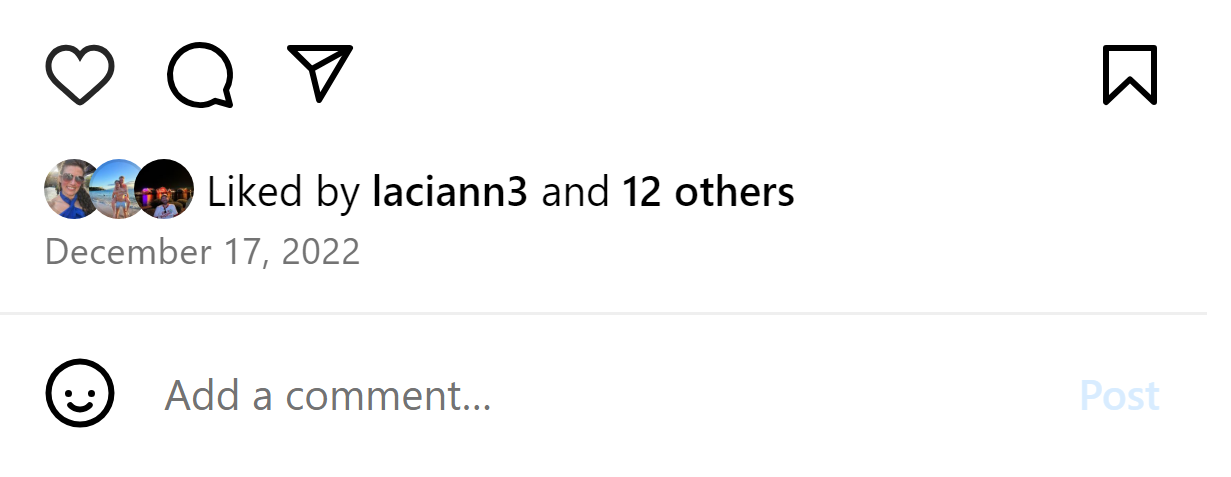
\includegraphics[width=1\textwidth,height=\textheight]{images/instagram_kpi-01.PNG}
\caption{\textbf{Instagram KPIs} (Source: @APLeithTV)}
\end{figure}

\hypertarget{customizing-kpis}{%
\subsubsection*{Customizing KPIs}\label{customizing-kpis}}
\addcontentsline{toc}{subsubsection}{Customizing KPIs}

It's also important to recognize that not all KPIs are one-size-fits-all. Customization of KPIs based on the unique nature and objectives of your business or campaign is crucial. This means taking into account factors like your industry, target audience, and the specific nuances of your brand or campaign. Customizing KPIs ensures that they are not just generic metrics, but meaningful indicators that provide real insights into the performance of your social media strategies. Tailoring these KPIs to your specific context will allow you to gather more relevant data, offering clearer insights and more actionable results.

The identification of relevant KPIs is a process that requires careful consideration of your social media goals, an understanding of common KPIs related to these goals, and the customization of these KPIs to fit the unique context of your business or campaign. By aligning KPIs with specific objectives and ensuring they are tailored to provide valuable insights, you can effectively measure the success of your social media strategies and make informed decisions to optimize your online presence.

\hypertarget{kpis-across-different-platforms}{%
\subsection*{KPIs Across Different Platforms}\label{kpis-across-different-platforms}}
\addcontentsline{toc}{subsection}{KPIs Across Different Platforms}

When delving into social media analytics, it becomes evident that each platform has its own set of dynamics and features that influence the choice and interpretation of Key Performance Indicators (KPIs). Understanding how these KPIs vary across different social media platforms is essential for accurately measuring and optimizing the impact of social media strategies.

\hypertarget{platform-specific-kpis}{%
\subsubsection*{Platform-Specific KPIs}\label{platform-specific-kpis}}
\addcontentsline{toc}{subsubsection}{Platform-Specific KPIs}

The selection of KPIs should be tailored to the specific characteristics and user engagement patterns of each platform. For example, on Facebook, `Shares' are a significant metric, indicating not only engagement but also the extent to which content resonates with users to the point of sharing it with their own networks. Similarly, Twitter's `Retweets' and `Mentions' are crucial KPIs, reflecting the spread and conversation around a piece of content. On Instagram, `Likes' and `Story Views' are key metrics, the former being a quick measure of content approval and the latter providing insight into the engagement with more temporary, day-to-day content. YouTube, with its focus on video content, places importance on `Watch Time' -- the total duration for which viewers have watched a video -- and subscriber growth, both indicative of the content's ability to attract and retain viewers over time.

\textbf{\emph{Twitch Chat Data}}

\begin{longtable}[]{@{}
  >{\raggedright\arraybackslash}p{(\columnwidth - 4\tabcolsep) * \real{0.1807}}
  >{\raggedright\arraybackslash}p{(\columnwidth - 4\tabcolsep) * \real{0.6024}}
  >{\raggedright\arraybackslash}p{(\columnwidth - 4\tabcolsep) * \real{0.2048}}@{}}
\toprule\noalign{}
\endhead
\bottomrule\noalign{}
\endlastfoot
\textbf{Variable} & \textbf{Description} & \textbf{Example} \\
id & Unique number given to each message. & 2573365 \\
channel & Name of channel in which message was sent. & \#lilypichu \\
sender & User who sent the message. & hunterlucian10 \\
message & Text of the message. & cmonBruh why \\
date & Date and time of chat message in Unix Timestamp & 1542607107593 \\
\end{longtable}

\emph{Note.} Pulled from the Twitch stream of Lilypichu on Nov 19, 2018.

\textbf{\emph{Twitch Stream Data}}

\begin{longtable}[]{@{}
  >{\raggedright\arraybackslash}p{(\columnwidth - 4\tabcolsep) * \real{0.1829}}
  >{\raggedright\arraybackslash}p{(\columnwidth - 4\tabcolsep) * \real{0.6098}}
  >{\raggedright\arraybackslash}p{(\columnwidth - 4\tabcolsep) * \real{0.1951}}@{}}
\toprule\noalign{}
\endhead
\bottomrule\noalign{}
\endlastfoot
\textbf{Variable} & \textbf{Description} & \textbf{Example} \\
id & Unique number given to each data pull. & 214439 \\
channel & Name of channel. & lilypichu \\
title & User who sent the message. & hello \\
game & Text of the message. & Just Chatting \\
viewers & Date and time of chat message in Unix Timestamp & 3607 \\
date & Date and time of data pull in Unix Timestamp & 1542754203847 \\
\end{longtable}

\emph{Note.} Pulled from the Twitch stream of Lilypichu on Nov 19, 2018.

\textbf{Twitter Data}

\begin{longtable}[]{@{}
  >{\raggedright\arraybackslash}p{(\columnwidth - 4\tabcolsep) * \real{0.1411}}
  >{\raggedright\arraybackslash}p{(\columnwidth - 4\tabcolsep) * \real{0.5031}}
  >{\raggedright\arraybackslash}p{(\columnwidth - 4\tabcolsep) * \real{0.3497}}@{}}
\toprule\noalign{}
\endhead
\bottomrule\noalign{}
\endlastfoot
\textbf{Variable} & \textbf{Description} & \textbf{Example} \\
tweet\_id & Unique numerical identifier for tweet. & 1494166530250010000 \\
user\_username & Twitter username of tweeter. & RubberNinja \\
text & Text of tweet. & @VRChat This is so cool! \\
in\_reply\_to\_user\_id & Numerical identifier of user who posted the tweet to which this is was a reply. & 2850482629 \\
lang & Language of tweet (abbreviated) & en \\
created\_at & Time tweet was posted (UTC) & 2022-02-17T04:27:15.000Z \\
author\_id & Unique numerical ID of tweeter. & 21076522 \\
conversation\_id & Unique numerical identifier of initial tweet in chain of tweets. & 1494152498617240000 \\
user\_location & Stated location of tweeter. & Los Angeles, CA \\
user\_name & Publicly displayed name of tweet poster. & RubberRoss \\
user\_description & Public description of tweeter. & \begin{minipage}[t]{\linewidth}\raggedright
My name is Ross O'Donovan, I draw and animate.\\
\url{https://t.co/05k3slkeDB} \textbar{} \url{https://t.co/EQro7JqnCD}\strut
\end{minipage} \\
user\_verified & Poster's verification status (Logical) & FALSE \\
retweet\_count & Number of retweets on this tweet. & 0 \\
like\_count & Number of likes on this tweet. & 70 \\
quote\_count & Number of quote tweets on this tweet. & 0 \\
user\_tweet\_count & Number of tweets posted by tweeter. & 31010 \\
user\_followers\_count & Number of followers of tweeter. & 689996 \\
user\_following\_count & Number of users that the tweeter follows. & 3803 \\
\end{longtable}

\emph{Note.} Not all available data is listed.

\hypertarget{understanding-platform-dynamics}{%
\subsubsection*{Understanding Platform Dynamics}\label{understanding-platform-dynamics}}
\addcontentsline{toc}{subsubsection}{Understanding Platform Dynamics}

Grasping the unique dynamics of each platform is vital in selecting and interpreting KPIs. These dynamics are shaped by the platform's design, user base, and typical content formats. For instance, YouTube's emphasis on video content means that KPIs related to view duration, such as average watch time, are particularly relevant. These metrics provide insights into viewer engagement and content quality. Similarly, on a platform like LinkedIn, where the focus is on professional networking and industry content, KPIs like `Profile Views' and `Connections' might take precedence, reflecting professional reach and network building.

This platform-specific approach to KPIs requires a deep understanding not only of the technical aspects of each platform but also of the behavioral patterns of their user bases. For example, high `Shares' on Facebook might indicate a successful content strategy that encourages community engagement and discussion, while a high number of `Retweets' on Twitter could signify the content's relevance to current trends or public discourse.

A nuanced approach to KPIs that considers the unique features and user engagement patterns of each social media platform is crucial. Such an approach allows for a more accurate and effective measurement of social media strategies, ensuring that the KPIs chosen are truly reflective of the platform's dynamics and can provide actionable insights into content performance and audience engagement.

\hypertarget{setting-and-benchmarking-kpis}{%
\subsection*{Setting and Benchmarking KPIs}\label{setting-and-benchmarking-kpis}}
\addcontentsline{toc}{subsection}{Setting and Benchmarking KPIs}

In the strategic realm of social media analytics, the process of setting and benchmarking Key Performance Indicators (KPIs) is vital for the success and relevance of social media efforts. This process ensures that the goals set are not only ambitious but also attainable, and grounded in a realistic understanding of the industry and the organization's capabilities.

\hypertarget{setting-realistic-kpis}{%
\subsubsection*{Setting Realistic KPIs}\label{setting-realistic-kpis}}
\addcontentsline{toc}{subsubsection}{Setting Realistic KPIs}

Setting realistic KPIs is a critical step in developing an effective social media strategy. This requires a careful assessment of several factors to ensure that the KPIs are not only challenging but also achievable. One of the key considerations is the current industry standards, which provide a benchmark for what is achievable and what constitutes success within a particular sector. Additionally, historical data from previous campaigns offers invaluable insights into what has been accomplished in the past and under what circumstances. This historical perspective can guide the setting of future KPIs by highlighting achievable targets based on past performance. Another important factor is the evaluation of the specific resources available, including budget, tools, and human resources, which can directly impact the feasibility of achieving certain KPIs.

\hypertarget{benchmarking-against-industry-standards}{%
\subsubsection*{Benchmarking Against Industry Standards}\label{benchmarking-against-industry-standards}}
\addcontentsline{toc}{subsubsection}{Benchmarking Against Industry Standards}

Benchmarking KPIs against industry standards and competitors is an essential practice in social media analytics. This involves an in-depth analysis of industry reports, competitor data, and leveraging tools that provide benchmarking data. By comparing an organization's KPIs with those of its peers and competitors, businesses can gain a clear understanding of where they stand in the industry landscape. This comparison can reveal strengths to be leveraged and weaknesses that need addressing, providing a roadmap for improvement and strategic adjustments. Benchmarking against industry standards also ensures that an organization's social media strategies are aligned with market realities and are competitive.

\hypertarget{regular-review-and-adjustment}{%
\subsubsection*{Regular Review and Adjustment}\label{regular-review-and-adjustment}}
\addcontentsline{toc}{subsubsection}{Regular Review and Adjustment}

The digital landscape, especially social media, is characterized by rapid changes and evolving trends. Therefore, it is essential to regularly review and adjust KPIs to align with these changes. This process involves regularly analyzing campaign performance, monitoring emerging trends in social media, and revising business objectives as needed. Regular review ensures that KPIs remain relevant and aligned with the current social media environment and business goals. Adjustments may involve redefining target metrics, shifting focus to different platforms, or revising strategies to better engage with the audience. This dynamic approach to KPI management is crucial for maintaining the effectiveness and relevance of social media strategies in an ever-changing digital landscape.

Setting realistic KPIs, benchmarking them against industry standards, and regularly reviewing and adjusting these indicators are fundamental practices in social media analytics. These processes ensure that social media efforts are strategically aligned, competitively positioned, and agile enough to adapt to the fast-paced nature of social media trends and market dynamics.

\hypertarget{measuring-engagement-reach-and-influence}{%
\section*{Measuring Engagement, Reach, and Influence}\label{measuring-engagement-reach-and-influence}}
\addcontentsline{toc}{section}{Measuring Engagement, Reach, and Influence}

In the intricate world of social media, understanding and accurately measuring key metrics like engagement, reach, and influence is essential for gauging the effectiveness of social media strategies. These metrics offer profound insights into audience interactions, the spread of content, and its overall impact. This section explores the nuances of these metrics, including their definitions, measurement tools and techniques, and the methodologies for their effective interpretation and analysis.

Engagement on social media is a measure of how users interact with content. It encompasses actions such as likes, comments, shares, and views. Engagement metrics are critical as they indicate not only the popularity of the content but also the extent to which it resonates with the audience. High engagement rates often suggest that the content is relevant, appealing, and provokes a reaction from the audience. To measure engagement, one can use native analytic tools provided by the social media platforms themselves, such as Facebook Insights or Instagram Analytics. These tools track the number of interactions and provide detailed breakdowns of engagement types.

Reach, another pivotal metric, refers to the total number of unique users who have seen a piece of content. Unlike engagement, which focuses on interactions, reach provides insights into the visibility and extent of content dissemination. It's a crucial metric for understanding the potential audience size and measuring brand awareness. Reach can be measured through the same native analytics tools, which provide data on how many users have seen a post or campaign. Understanding reach helps in assessing the effectiveness of content distribution strategies and the platform's algorithm in content promotion.

Influence, while more nuanced, is about the capacity of the content or the social media presence to affect audience behavior or opinions. Influence can be reflected in various forms, such as the growth in follower count, the extent to which content is shared beyond the immediate audience, and conversions or actions taken as a result of the content. Measuring influence often involves a combination of quantitative data (like follower growth rate and share metrics) and qualitative insights (like audience feedback and sentiment analysis). Tools for measuring influence include both platform-specific analytics and third-party tools that offer deeper insights into audience behavior and content impact.

Effectively measuring and analyzing these metrics requires a blend of using the right tools, understanding the nuances of each metric, and aligning them with the objectives of the social media strategy. For instance, a campaign focused on brand awareness would prioritize reach and influence, while one aimed at community building would look closely at engagement metrics. The key is to interpret these metrics in the context of specific goals and the overarching social media strategy.

Engagement, reach, and influence are indispensable metrics in social media analytics. Accurately measuring and analyzing these metrics provide valuable insights into how content performs, how it resonates with audiences, and the overall impact of social media efforts. This understanding is crucial for crafting effective strategies, optimizing content, and achieving desired outcomes in the competitive landscape of social media.

\hypertarget{defining-reach-engagement-and-influence}{%
\subsection*{Defining Reach, Engagement, and Influence}\label{defining-reach-engagement-and-influence}}
\addcontentsline{toc}{subsection}{Defining Reach, Engagement, and Influence}

In the field of social media analytics, three key metrics stand out as essential gauges of content and campaign success: engagement, reach, and influence. Each of these metrics offers distinct insights into how users interact with and respond to social media content, and they are pivotal in shaping effective social media strategies.

\hypertarget{reach}{%
\subsubsection*{Reach}\label{reach}}
\addcontentsline{toc}{subsubsection}{Reach}

Reach refers to the total number of unique users who have seen a particular piece of content on social media. It is a vital metric for measuring the visibility and extent of content dissemination. Unlike engagement, which focuses on the depth of interaction with the content, reach is about the breadth of content exposure. It offers insights into the scale at which content is being seen and is crucial for campaigns focusing on brand awareness and exposure. Reach can be affected by various factors, including the platform's algorithm, the timing of the post, and the inherent appeal of the content. Understanding reach is fundamental for strategists looking to maximize their content's visibility across the social media landscape.

\hypertarget{engagement}{%
\subsubsection*{Engagement}\label{engagement}}
\addcontentsline{toc}{subsubsection}{Engagement}

Engagement on social media is a comprehensive term that encompasses how users interact with content. This interaction can take various forms, such as likes, comments, shares, and views. Likes indicate a basic level of user approval or interest, comments reflect a deeper level of engagement with the potential for dialogue, shares signify the content's appeal to the extent that users want to disseminate it within their networks, and views are essential for understanding the overall reach and impact, especially of video content. Engagement metrics are critical because they provide a direct indicator of how compelling, relevant, and resonant the content is with the audience. High engagement rates are often correlated with content that effectively captures and retains the audience's attention, sparking interest, and encouraging interaction.

\begin{figure}
\centering

\includegraphics[width=1\textwidth,height=\textheight]{images/engagement.jpg}
\caption{\textbf{Social Media Engagement} (Source: The Brandon Agency)}
\end{figure}

\hypertarget{influence}{%
\subsubsection*{Influence}\label{influence}}
\addcontentsline{toc}{subsubsection}{Influence}

Influence in social media pertains to the capacity of content or an account to affect the behavior or opinions of the audience. This metric is closely linked to the credibility and authority of the content creator or brand. Influence can be seen in various forms, such as the growth in follower count, indicating an increasing audience base; the virality of content, where the content spreads rapidly and widely across platforms; and conversions, where the content leads to specific user actions like website visits, sign-ups, or purchases. Influence is a nuanced metric that combines the elements of reach and engagement to reflect the overall impact and persuasive power of social media content.

Understanding reach, engagement, and influence is fundamental for anyone engaged in social media analytics. These metrics provide a comprehensive picture of how content is performing, how far it is reaching, and the extent of its impact on the audience. They are critical tools for assessing the effectiveness of social media strategies and guiding decisions to optimize content for maximum engagement and influence.

\hypertarget{techniques-and-tools-for-measurement}{%
\subsection*{Techniques and Tools for Measurement}\label{techniques-and-tools-for-measurement}}
\addcontentsline{toc}{subsection}{Techniques and Tools for Measurement}

In the realm of social media analytics, the selection and use of appropriate tools and techniques for measuring key metrics like engagement, reach, and influence are essential. These tools range from native analytics provided by social media platforms to sophisticated third-party analytical tools, each offering distinct features and capabilities. Understanding these tools and selecting the right ones based on specific needs and goals are crucial steps in effective social media analytics.

\hypertarget{analytical-tools-introduction}{%
\subsubsection*{Analytical Tools Introduction}\label{analytical-tools-introduction}}
\addcontentsline{toc}{subsubsection}{Analytical Tools Introduction}

Each major social media platform offers its own set of native analytics tools, designed to provide insights into the performance of content and campaigns on their respective platforms. Facebook Insights, for instance, offers in-depth data on page performance, audience demographics, and engagement metrics. Twitter Analytics provides valuable insights into tweet performance, audience interests, and engagement trends. Instagram Insights delivers data on follower demographics, post performance, and stories analytics. LinkedIn Analytics, on the other hand, focuses on professional audience engagement, content reach, and page growth metrics. These native tools are essential for any social media strategy as they provide specific data directly from the source, enabling a clear understanding of how content performs on each platform.

\hypertarget{third-party-analytical-tools}{%
\subsubsection*{Third-Party Analytical Tools}\label{third-party-analytical-tools}}
\addcontentsline{toc}{subsubsection}{Third-Party Analytical Tools}

In addition to native analytics, there are numerous third-party tools available that offer more advanced analytics and integrated insights across multiple platforms. Tools like Hootsuite, Google Analytics, and Sprout Social are widely used in the industry. Hootsuite, for example, allows for comprehensive monitoring and management of multiple social media accounts in one place, offering analytics that helps track key metrics, schedule posts, and engage with audiences. Google Analytics is instrumental in tracking website traffic from social media platforms, providing insights into user behavior, conversions, and the effectiveness of social media campaigns in driving web traffic. Sprout Social offers detailed analytics, social listening, and engagement tools, helping businesses to understand and interact with their audience more effectively. These third-party tools are valuable for their ability to consolidate data from various sources and provide a more holistic view of social media performance.

\begin{figure}
\centering
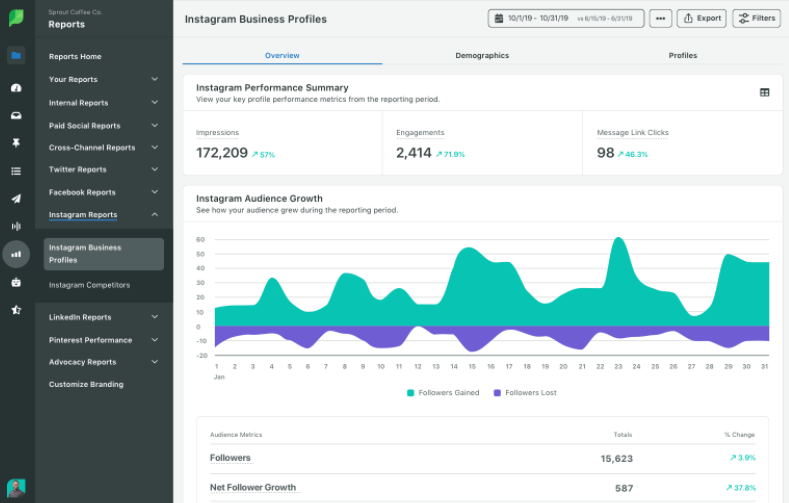
\includegraphics[width=1\textwidth,height=\textheight]{images/sprout.png}
\caption{\textbf{Sprout Social} (Source: Digital Marketer's World)}
\end{figure}

\hypertarget{tool-selection-criteria}{%
\subsubsection*{Tool Selection Criteria}\label{tool-selection-criteria}}
\addcontentsline{toc}{subsubsection}{Tool Selection Criteria}

When selecting the most appropriate tools for social media measurement, several criteria need to be considered. Platform coverage is essential; the tool should support analytics for all the platforms used in your social media strategy. The depth of analytics is another critical factor - the tool should provide detailed insights that go beyond basic metrics to include audience analysis, competitor analysis, and trend tracking. Real-time tracking capabilities are also crucial for monitoring ongoing campaigns and responding promptly to engagement opportunities. Finally, the ease of use and user interface of the tool should be considered to ensure efficiency and usability for all team members.

A comprehensive understanding and careful selection of analytical tools are fundamental for effective social media measurement. By leveraging the strengths of both native and third-party tools and choosing them based on specific criteria, social media professionals can gain deep insights, drive strategy, and optimize their social media presence effectively.

\hypertarget{engagement-metrics-and-their-interpretation}{%
\subsection*{Engagement Metrics and Their Interpretation}\label{engagement-metrics-and-their-interpretation}}
\addcontentsline{toc}{subsection}{Engagement Metrics and Their Interpretation}

In the landscape of social media, understanding and interpreting engagement metrics is vital for assessing how users interact with content. These metrics offer insights into the effectiveness of social media strategies, user behavior, and content performance. This section delves into the various types of engagement metrics, the techniques for measuring them, and the methodologies for interpreting this data to inform future strategies.

\hypertarget{types-of-engagement-metrics}{%
\subsubsection*{Types of Engagement Metrics}\label{types-of-engagement-metrics}}
\addcontentsline{toc}{subsubsection}{Types of Engagement Metrics}

Engagement metrics in social media encompass a range of indicators that show how users are interacting with content. Likes, for example, are a basic yet powerful metric indicating user approval or interest. Comment rates go a step further, showing not just interest but active engagement and willingness to participate in a conversation or express opinions. Share counts are particularly significant, as they indicate that the content resonated strongly enough with users that they chose to spread it within their own networks. Finally, video view statistics are essential in the age of digital media, providing insights into how long users are engaging with video content, which is increasingly becoming the most consumed type of content online. Each of these metrics offers specific insights into user interaction and is crucial for evaluating the success of social media content.

\hypertarget{measurement-techniques}{%
\subsubsection*{Measurement Techniques}\label{measurement-techniques}}
\addcontentsline{toc}{subsubsection}{Measurement Techniques}

To effectively measure these engagement metrics, one must utilize the tools and techniques available through both native and third-party analytics platforms. Tracking engagement trends over time allows for an understanding of how engagement evolves in response to different content strategies or external factors. Comparing engagement across different content types can highlight what resonates best with your audience, whether it be text posts, images, or videos. Understanding peak engagement times is also crucial; it involves analyzing when your audience is most active on the platform, which can greatly impact the visibility and engagement of your posts. Regularly monitoring these metrics enables a dynamic approach to content strategy, allowing for adjustments and optimizations based on real-time feedback and trends.

\hypertarget{interpreting-engagement-data}{%
\subsubsection*{Interpreting Engagement Data}\label{interpreting-engagement-data}}
\addcontentsline{toc}{subsubsection}{Interpreting Engagement Data}

The interpretation of engagement data is where the real analytical skill comes into play. High engagement rates might indicate that your content is highly relevant and appealing to your audience, but it's important to dive deeper. Understanding what different levels and types of engagement indicate about your content's performance is crucial. For instance, a high number of likes but few comments might suggest that while the content is well-received, it may not be provocative or engaging enough to spark a conversation. Analyzing comment sentiment can provide insights into audience preferences and content relevance. Similarly, understanding the context behind share counts can offer clues about the content's ability to generate interest or controversy. Interpreting these metrics in the context of your overall content strategy, audience demographics, and platform trends is key to gaining actionable insights that can drive more effective social media strategies.

Engagement metrics are fundamental to understanding how users interact with social media content. By effectively measuring and interpreting these metrics, social media professionals can gain a deeper understanding of their audience, refine their content strategies, and enhance their overall social media presence. This process involves not just the collection of data but also its careful analysis to draw meaningful insights that can inform future strategies.

\hypertarget{reach-and-influence-analysis}{%
\subsection*{Reach and Influence Analysis}\label{reach-and-influence-analysis}}
\addcontentsline{toc}{subsection}{Reach and Influence Analysis}

In the domain of social media analytics, understanding and analyzing reach and influence is crucial for evaluating the effectiveness of content and campaigns. Reach refers to the extent to which content is seen by users, while influence pertains to the content's ability to affect user behavior or opinions. This section explores the methodologies for calculating reach, measuring influence, and includes case studies to illustrate successful strategies in these areas.

\hypertarget{calculating-reach}{%
\subsubsection*{Calculating Reach}\label{calculating-reach}}
\addcontentsline{toc}{subsubsection}{Calculating Reach}

Reach on social media can be broadly categorized into organic reach and paid reach. Organic reach refers to the number of unique users who see your content without paid promotion. It is influenced by various factors such as the content's relevance, the time of posting, and the platform's algorithm. Organic reach is often seen as a measure of the natural appeal and quality of the content. On the other hand, paid reach involves using paid advertising to increase the visibility of content. It can be targeted based on specific demographics, interests, and behaviors, and is often used to boost exposure to new or wider audiences. Understanding these different types of reach and the factors that influence them is essential for developing strategies to maximize the visibility of social media content.

\hypertarget{influence-measurement}{%
\subsubsection*{Influence Measurement}\label{influence-measurement}}
\addcontentsline{toc}{subsubsection}{Influence Measurement}

Measuring the influence of social media content and campaigns involves assessing the impact on audience behavior and opinions. This can be gauged through various metrics, such as the level of engagement (likes, comments, shares), the growth in follower count, and the extent of content virality. The role of influencers -- individuals with significant followings and the ability to sway their audience -- is also critical in influence measurement. Influencer partnerships can amplify a campaign's reach and impact. Additionally, the significance of user-generated content in driving engagement and fostering community participation is another aspect of measuring influence. Moreover, conversions resulting from social media interactions, such as website visits, sign-ups, or purchases, are tangible indicators of the campaign's influence on user behavior.

\hypertarget{interpreting-metrics-for-strategic-insights}{%
\section*{Interpreting Metrics for Strategic Insights}\label{interpreting-metrics-for-strategic-insights}}
\addcontentsline{toc}{section}{Interpreting Metrics for Strategic Insights}

\hypertarget{interpreting-metrics-for-strategic-insights-1}{%
\section{Interpreting Metrics for Strategic Insights}\label{interpreting-metrics-for-strategic-insights-1}}

In the constantly evolving digital landscape, the ability to effectively interpret and utilize social media metrics for strategic insights is indispensable. Social media platforms generate a vast amount of raw data, but the real value lies in transforming this data into actionable insights that can guide business strategies and decisions. This crucial aspect of social media analytics involves not only understanding what the data represents but also how it can be applied to meet business objectives. This section delves into the methodologies for analyzing social media metrics, supplemented with case studies for practical application, and highlights the importance of continuous monitoring and adaptation of strategies based on these insights.

Firstly, interpreting metrics requires a deep understanding of what each metric represents and its relevance to specific business goals. For example, a high number of likes or shares may indicate content popularity, but it's essential to analyze further to understand the implications for brand awareness or customer engagement. Engagement rates, click-through rates, and conversion rates are often more telling metrics, providing deeper insights into audience behavior and the effectiveness of content strategies.

The analysis of these metrics should be methodical and aligned with the business's overall objectives. For instance, if the goal is to increase brand awareness, analyzing reach and impressions will be more relevant. If the aim is to drive sales, then conversion rates and click-through rates will be key metrics to focus on. This targeted analysis helps in making informed decisions about content strategy, marketing campaigns, and audience engagement tactics.

Case studies serve as valuable tools for understanding the practical application of these metrics. They provide real-world examples of how businesses have successfully leveraged social media metrics to achieve their objectives, or how a misinterpretation of these metrics led to less than favorable outcomes. Learning from these case studies, both successes and failures, can provide critical insights and guide strategy formulation.

The dynamic nature of social media means that continuous monitoring and adjustment of strategies are essential. Social media trends, platform algorithms, and audience preferences can change rapidly. Regular analysis of KPIs and other metrics allows businesses to stay agile, making necessary adjustments to their strategies in real-time. This might involve shifting focus between different platforms, altering content types, or modifying engagement tactics based on the latest data.

Interpreting social media metrics for strategic insights is a multifaceted process that involves understanding each metric's significance, aligning them with business goals, learning from practical examples, and continually adapting strategies based on ongoing analysis. This approach ensures that businesses can not only track the performance of their social media efforts but also gain valuable insights that drive growth and improvement in their digital marketing strategies.

\hypertarget{translating-metrics-into-actionable-insights}{%
\subsection*{Translating Metrics into Actionable Insights}\label{translating-metrics-into-actionable-insights}}
\addcontentsline{toc}{subsection}{Translating Metrics into Actionable Insights}

In the realm of social media analytics, the ability to translate metrics into actionable insights is crucial for refining strategies and achieving desired outcomes. This process involves a comprehensive analysis of data, recognition of patterns, and the application of these insights to enhance social media planning and execution. This section explores the methodologies for data analysis, techniques for pattern recognition, and ways to turn data into effective strategy.

\hypertarget{methodologies-for-data-analysis}{%
\subsubsection*{Methodologies for Data Analysis}\label{methodologies-for-data-analysis}}
\addcontentsline{toc}{subsubsection}{Methodologies for Data Analysis}

Analyzing social media data requires a robust understanding of various analytical methodologies that can uncover meaningful insights from metrics. Trend analysis is a fundamental technique that involves examining data over time to identify consistent patterns or anomalies. For example, a steady increase in engagement rates might indicate growing audience interest or the effectiveness of a particular content strategy. Comparative analysis is another critical method, allowing for the comparison of different data sets, such as engagement rates across different platforms or time periods. This analysis helps in understanding what strategies work best and where there might be room for improvement. Correlation studies involve examining the relationship between different variables, for instance, how changes in posting frequency might correlate with engagement rates. Understanding these relationships helps in identifying what factors most significantly impact campaign performance and user behavior.

\hypertarget{pattern-recognition-in-metrics}{%
\subsubsection*{Pattern Recognition in Metrics}\label{pattern-recognition-in-metrics}}
\addcontentsline{toc}{subsubsection}{Pattern Recognition in Metrics}

Recognizing patterns within social media metrics is key to identifying both opportunities and potential issues. This involves a detailed examination of metrics to detect shifts in user engagement, content performance, and audience demographics. For instance, a sudden spike in engagement on specific types of posts can reveal emerging content preferences of the audience. Similarly, changes in audience demographics, such as a shift in the age or geographical location of the majority of followers, can indicate evolving audience dynamics and help in tailoring content accordingly. Recognizing these patterns enables social media analysts to anticipate trends, adapt strategies, and address any emerging issues proactively.

\hypertarget{turning-data-into-strategy}{%
\subsubsection*{Turning Data into Strategy}\label{turning-data-into-strategy}}
\addcontentsline{toc}{subsubsection}{Turning Data into Strategy}

The ultimate goal of analyzing social media metrics is to turn these insights into an effective strategy. Data-driven insights can significantly inform content strategy, helping determine what type of content resonates most with the audience, the ideal posting schedule, and the most effective content formats. Audience targeting can also be refined based on demographic insights and user behavior patterns, ensuring that content reaches and engages the most relevant audience. Overall social media planning benefits from these insights, as they guide decision-making in content creation, platform selection, and engagement tactics. By integrating these insights into the planning process, social media strategies can become more focused, responsive, and effective in achieving their objectives.

Translating metrics into actionable insights involves a comprehensive analysis of social media data, recognition of important patterns, and the application of these insights to refine and enhance social media strategies. This process is crucial for navigating the dynamic landscape of social media and for ensuring that social media efforts are strategically aligned and capable of achieving desired results.

\hypertarget{aligning-metrics-with-business-objectives}{%
\subsection*{Aligning Metrics with Business Objectives}\label{aligning-metrics-with-business-objectives}}
\addcontentsline{toc}{subsection}{Aligning Metrics with Business Objectives}

In the strategic practice of social media analytics, aligning metrics with business objectives is pivotal for ensuring that social media efforts contribute effectively to overarching goals. This section emphasizes the importance of this alignment and offers guidance on adjusting strategies based on metric analysis to optimize performance.

\hypertarget{importance-of-alignment}{%
\subsubsection*{Importance of Alignment}\label{importance-of-alignment}}
\addcontentsline{toc}{subsubsection}{Importance of Alignment}

The alignment of social media metrics with business or campaign objectives is critical for the success of any digital marketing effort. Social media metrics should not be viewed in isolation but rather as indicators that inform and reflect the broader business goals. For instance, if the objective is to enhance brand awareness, metrics like reach, impressions, and follower growth rate are particularly relevant as they provide insights into the brand's visibility and recognition. For objectives such as lead generation, metrics like click-through rates and conversion rates become more crucial, as they directly relate to the effectiveness of social media in generating potential customer leads. Similarly, for goals centered around customer engagement or sales, metrics like engagement rates and direct inquiries or sales through social media channels are key indicators of success. This alignment ensures that every aspect of a social media strategy is geared towards and measured against the specific goals it aims to achieve.

\hypertarget{adjusting-strategies-based-on-metrics}{%
\subsubsection*{Adjusting Strategies Based on Metrics}\label{adjusting-strategies-based-on-metrics}}
\addcontentsline{toc}{subsubsection}{Adjusting Strategies Based on Metrics}

Analyzing social media metrics offers valuable insights that can inform the adjustment and refinement of strategies. Based on metric performance, content strategies may need to be refined. For example, if video content consistently shows higher engagement rates, the strategy might shift to include more video content. If certain types of posts are seen to drive higher conversion rates, they can be prioritized in content planning. Targeting efforts might also be adjusted based on insights into audience demographics and behaviors derived from social media metrics. If data shows that a particular demographic is more engaged or more likely to convert, targeting strategies can be honed to focus more on that segment. Engagement tactics, such as the timing of posts, frequency, and types of interactions, can also be optimized based on metrics. For example, if engagement peaks at specific times, posting schedules can be adjusted accordingly.

The alignment of social media metrics with business objectives is essential for ensuring that social media activities are focused and effective. Regular analysis of these metrics allows for strategic adjustments and optimizations, ensuring that the social media strategy remains aligned with and conducive to achieving the desired business outcomes. This ongoing process of alignment and adjustment is a critical component of successful social media analytics and strategy.

\hypertarget{continuous-monitoring-and-adjustment}{%
\subsection*{Continuous Monitoring and Adjustment}\label{continuous-monitoring-and-adjustment}}
\addcontentsline{toc}{subsection}{Continuous Monitoring and Adjustment}

In the fast-paced and ever-evolving world of social media, continuous monitoring and strategic adjustment based on analytics are essential for maintaining the relevance and effectiveness of social media strategies. This section underscores the necessity of ongoing analysis, provides recommendations for setting up regular reporting structures, and discusses the importance of strategic pivoting based on insights gleaned from social media metrics.

\hypertarget{the-need-for-ongoing-analysis}{%
\subsubsection*{The Need for Ongoing Analysis}\label{the-need-for-ongoing-analysis}}
\addcontentsline{toc}{subsubsection}{The Need for Ongoing Analysis}

Continuous monitoring of social media metrics is crucial, as the digital landscape and user behaviors are constantly changing. Relying solely on one-time analysis can lead to outdated strategies that fail to resonate with the current audience. Ongoing analysis allows for the identification of trends, shifts in audience preferences, and emerging opportunities or challenges. By consistently tracking metrics such as engagement rates, reach, follower growth, and conversion rates, businesses can gain a real-time understanding of their social media performance. This continuous monitoring enables timely responses to changes in the social media environment, ensuring that strategies remain aligned with current user behaviors and platform algorithms.

\hypertarget{recommendations-for-regular-reporting}{%
\subsubsection*{Recommendations for Regular Reporting}\label{recommendations-for-regular-reporting}}
\addcontentsline{toc}{subsubsection}{Recommendations for Regular Reporting}

To effectively implement continuous monitoring, it is recommended to establish regular reporting structures. These can take the form of weekly or monthly performance reviews, depending on the scale and dynamics of the social media activities. Regular reporting should encompass a comprehensive analysis of key metrics, comparisons against previous periods, and benchmarking against industry standards or competitors. Utilizing dashboards and analytical tools can simplify the process, providing clear and accessible insights into performance trends. These reports should not only present data but also offer actionable insights and recommendations for strategy adjustments. Regular reporting ensures that stakeholders are kept informed and that strategic decisions are data-driven.

\hypertarget{strategic-pivoting-based-on-insights}{%
\subsubsection*{Strategic Pivoting Based on Insights}\label{strategic-pivoting-based-on-insights}}
\addcontentsline{toc}{subsubsection}{Strategic Pivoting Based on Insights}

The ability to pivot strategies based on insights from ongoing analysis is a critical aspect of agile social media management. Insights gained from continuous monitoring should inform strategic decisions, allowing businesses to adapt to the changing digital landscape swiftly. This might involve reallocating resources to more effective channels if certain platforms are underperforming, experimenting with new types of content that are resonating with the audience, or adjusting targeting criteria to better reach the desired demographic. Strategic pivoting based on real-time data allows businesses to capitalize on emerging trends, mitigate risks, and optimize the ROI of their social media efforts.

Continuous monitoring and the ability to adjust strategies based on ongoing insights are fundamental for the success of social media initiatives. By embracing a dynamic approach to social media analytics, businesses can ensure that their strategies are responsive, relevant, and effective in achieving their desired social media objectives.

\hypertarget{studying-successful-social-media-campaigns}{%
\chapter{Studying Successful Social Media Campaigns}\label{studying-successful-social-media-campaigns}}

\hypertarget{analysis-of-successful-campaigns-across-various-platforms}{%
\section*{Analysis of Successful Campaigns Across Various Platforms}\label{analysis-of-successful-campaigns-across-various-platforms}}
\addcontentsline{toc}{section}{Analysis of Successful Campaigns Across Various Platforms}

\hypertarget{case-study-selection-and-criteria}{%
\subsection*{Case Study Selection and Criteria}\label{case-study-selection-and-criteria}}
\addcontentsline{toc}{subsection}{Case Study Selection and Criteria}

\hypertarget{level-of-engagement}{%
\subsubsection*{Level of Engagement}\label{level-of-engagement}}
\addcontentsline{toc}{subsubsection}{Level of Engagement}

Engagement metrics are crucial indicators of a campaign's resonance with its audience. Metrics such as likes, shares, comments, and views offer quantifiable evidence of how users interact with and respond to social media content. High engagement rates typically suggest that the content is effective in capturing and retaining the audience's interest. Analyzing these metrics can reveal insights into the types of content that resonate most with users, optimal posting times, and the overall effectiveness of the campaign's communication strategy.

\hypertarget{achievement-of-specific-goals}{%
\subsubsection*{Achievement of Specific Goals}\label{achievement-of-specific-goals}}
\addcontentsline{toc}{subsubsection}{Achievement of Specific Goals}

The success of a campaign is also measured by how well it meets its predefined objectives. These objectives can range from increasing brand awareness and driving sales to advocating for social causes or fostering community engagement. This criterion involves evaluating the extent to which the campaign's goals were achieved and understanding the strategies that contributed to this success. For instance, a campaign aimed at driving sales would be assessed on metrics like conversion rates and revenue growth, while a campaign focused on raising awareness might be evaluated based on reach and public engagement.

\hypertarget{creativity-and-innovation}{%
\subsubsection*{Creativity and Innovation}\label{creativity-and-innovation}}
\addcontentsline{toc}{subsubsection}{Creativity and Innovation}

Creativity and innovation in campaign design and execution play a pivotal role in standing out in the crowded social media landscape. This includes novel uses of social media features, creative content strategies, and innovative engagement tactics. Campaigns that leverage these aspects effectively often achieve higher engagement and can set new trends in social media marketing. The evaluation of creativity and innovation requires not only an analysis of the campaign's content and strategies but also an understanding of the context and standards of the time when the campaign was executed.

\hypertarget{sustainability-and-long-term-impact}{%
\subsubsection*{Sustainability and Long-term Impact}\label{sustainability-and-long-term-impact}}
\addcontentsline{toc}{subsubsection}{Sustainability and Long-term Impact}

The long-term impact and sustainability of a campaign are significant indicators of success. This involves looking beyond immediate metrics to understand the enduring effects on brand perception, customer loyalty, and community engagement. A campaign with a lasting impact not only achieves its immediate goals but also contributes to the long-term growth and stability of the brand or cause it represents. This criterion assesses how the campaign has influenced the target audience over time and the extent to which it has fostered ongoing engagement and support.

Selecting case studies based on these criteria will provide comprehensive insights into the various factors that contribute to the success of social media campaigns. This approach ensures a balanced analysis, encompassing both quantitative metrics and qualitative aspects of campaign execution and impact.

\hypertarget{diverse-platform-analysis}{%
\subsection*{Diverse Platform Analysis}\label{diverse-platform-analysis}}
\addcontentsline{toc}{subsection}{Diverse Platform Analysis}

In the chapter ``Studying Successful Social Media Campaigns,'' it is essential to explore how different social media platforms contribute to the success of various campaigns. Each platform has unique features and caters to specific audience demographics, making an understanding of these distinctions crucial for effective campaign planning and analysis. This section delves into how successful campaigns have utilized the distinct characteristics of various platforms to maximize their impact.

\hypertarget{facebook}{%
\subsubsection*{Facebook}\label{facebook}}
\addcontentsline{toc}{subsubsection}{Facebook}

Facebook, known for its broad demographic reach and sophisticated targeting options, allows campaigns to connect with a diverse audience. Dove's ``Real Beauty Sketches'' campaign effectively utilized Facebook to promote its message of body positivity and self-esteem. By leveraging Facebook's targeting capabilities, the campaign could reach a wide range of demographics, resonating with a diverse audience and sparking meaningful conversations about beauty standards.

\begin{figure}
\centering
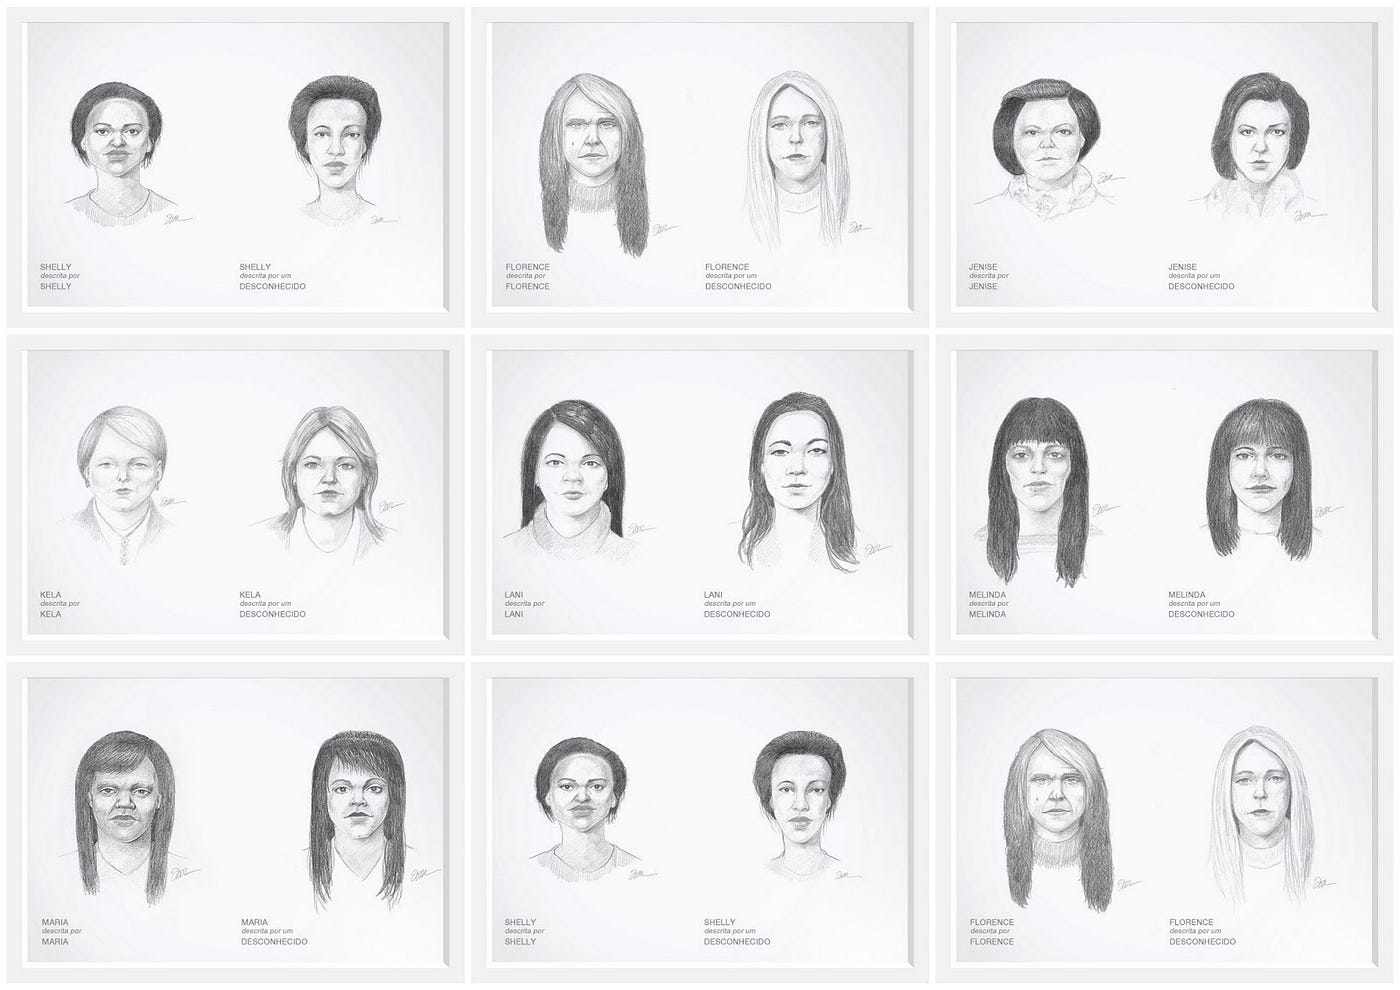
\includegraphics[width=1\textwidth,height=\textheight]{images/dove.jpg}
\caption{Dove: Real Beauty Sketches}
\end{figure}

\hypertarget{twitter}{%
\subsubsection*{Twitter}\label{twitter}}
\addcontentsline{toc}{subsubsection}{Twitter}

Twitter excels in facilitating real-time communication and the widespread use of hashtags, making it ideal for engaging campaigns and viral content. The ``\#NuggsForCarter'' campaign by Wendy's demonstrated Twitter's power in driving viral content. The campaign's clever use of a personal challenge, combined with a strategic hashtag, led to record-breaking engagement and elevated brand visibility.

\begin{figure}
\centering
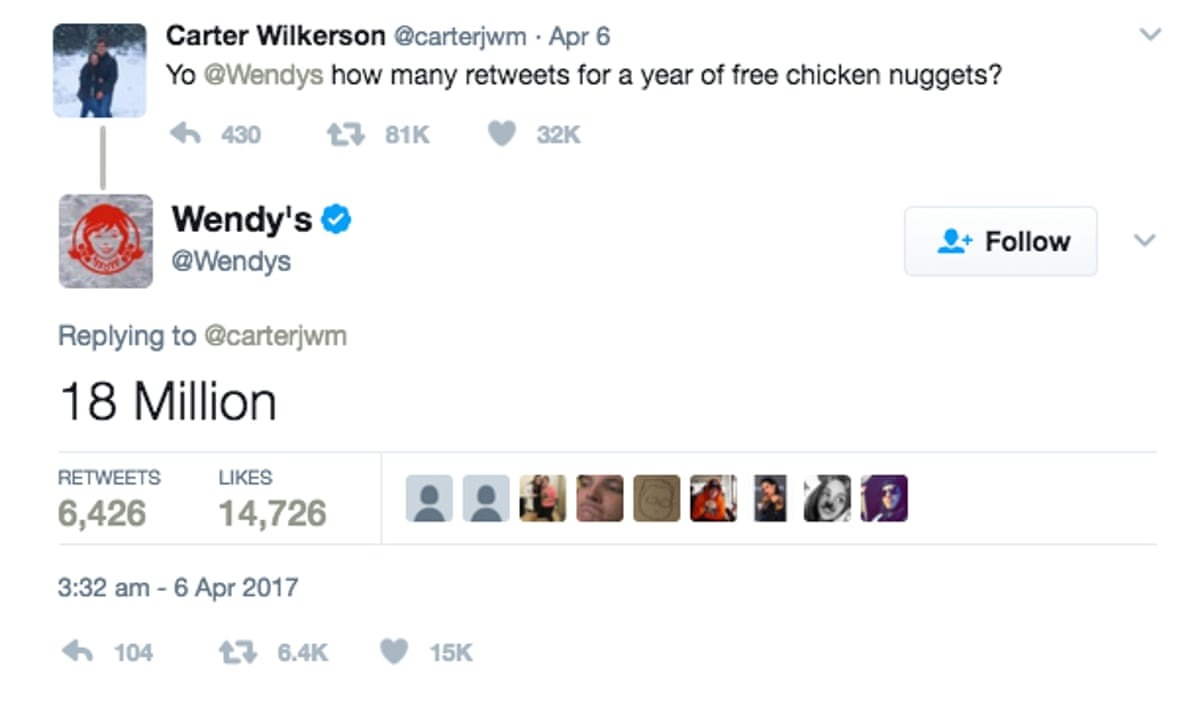
\includegraphics[width=1\textwidth,height=\textheight]{images/wendys.jpg}
\caption{Wendy's \#NuggsForCarter}
\end{figure}

\hypertarget{instagram}{%
\subsubsection*{Instagram}\label{instagram}}
\addcontentsline{toc}{subsubsection}{Instagram}

Instagram's strength lies in its visual-centric approach, allowing for powerful storytelling through imagery. National Geographic's use of Instagram exemplifies effective storytelling through captivating visuals. Their posts, which often feature stunning photography and engaging narratives, attract a vast audience interested in travel, nature, and culture.

\begin{figure}
\centering
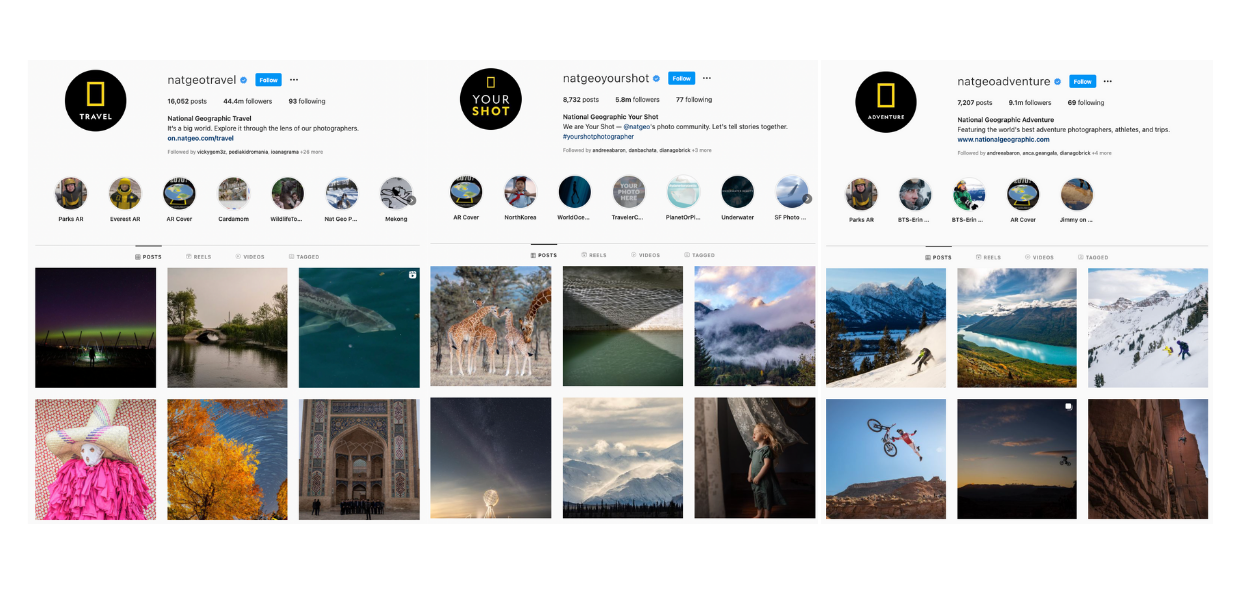
\includegraphics[width=1\textwidth,height=\textheight]{images/natgeo.png}
\caption{National Geographic: Themed Accounts}
\end{figure}

\hypertarget{linkedin}{%
\subsubsection*{LinkedIn}\label{linkedin}}
\addcontentsline{toc}{subsubsection}{LinkedIn}

LinkedIn's professional network is optimal for campaigns targeting business professionals and job seekers. Upwork's campaign on LinkedIn strategically leveraged the platform's professional user base. By showcasing a carousel of potential jobs, Upwork effectively connected with both companies seeking employees and professionals looking for opportunities, thus reinforcing its position as a leading freelancing platform.

\begin{figure}
\centering
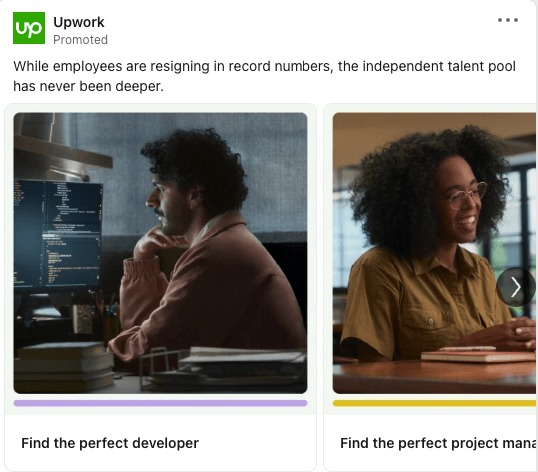
\includegraphics[width=0.75\textwidth,height=\textheight]{images/upwork.jpg}
\caption{Upwork: Assisting Job Seekers}
\end{figure}

\hypertarget{tiktok}{%
\subsubsection*{TikTok}\label{tiktok}}
\addcontentsline{toc}{subsubsection}{TikTok}

TikTok, known for its short-form videos and trend-driven content, appeals predominantly to a younger audience. Chipotle's ``\#LidFlipChallenge'' brilliantly capitalized on TikTok's format and user demographics. The challenge engaged users in a fun, interactive way, aligning perfectly with the platform's trend-centric nature and youthful audience.

\begin{figure}
\centering
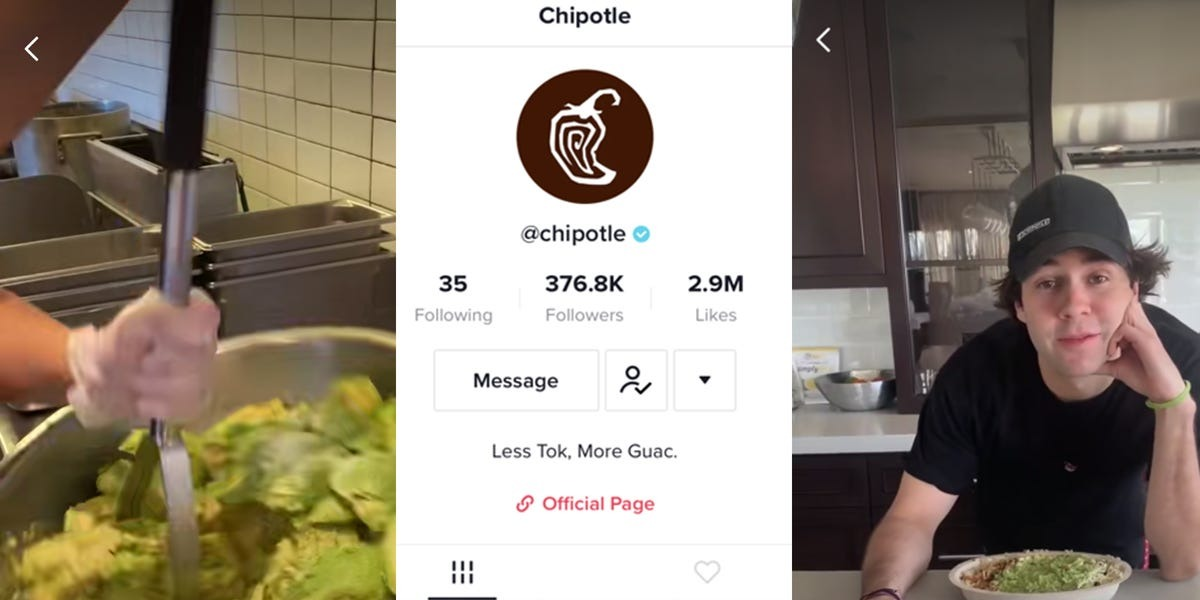
\includegraphics[width=1\textwidth,height=\textheight]{images/chipotle.jpg}
\caption{Chipotle: \#LidFlipChallenge}
\end{figure}

\hypertarget{youtube}{%
\subsubsection*{YouTube}\label{youtube}}
\addcontentsline{toc}{subsubsection}{YouTube}

YouTube's focus on video content allows for in-depth storytelling and the development of comprehensive narrative campaigns. The ``Like a Girl'' campaign by Always used YouTube's video platform to challenge gender stereotypes through emotional storytelling. The campaign's impactful narrative was well-suited to YouTube's format, enabling it to reach a wide audience and generate significant discussion.

\begin{figure}
\centering

\includegraphics[width=1\textwidth,height=\textheight]{images/always.jpg}
\caption{Always: Like a Girl}
\end{figure}

In summary, understanding the unique attributes of each social media platform is crucial for crafting successful campaigns. By analyzing how different platforms have been leveraged in these examples, insights can be gained into the strategies that work best for each social media environment.

\hypertarget{campaign-goals-and-strategies}{%
\subsection*{Campaign Goals and Strategies}\label{campaign-goals-and-strategies}}
\addcontentsline{toc}{subsection}{Campaign Goals and Strategies}

\hypertarget{brand-awareness}{%
\subsubsection*{Brand Awareness}\label{brand-awareness}}
\addcontentsline{toc}{subsubsection}{Brand Awareness}

The goal of increasing brand awareness is often at the forefront of many social media campaigns. Strategies employed for this purpose need to capture the attention of a broad audience and create a memorable impression of the brand.

\textbf{\emph{Strategies}}:

\begin{itemize}
\tightlist
\item
  \textbf{Viral Content Creation}: Crafting content that has the potential to go viral, thus reaching a wider audience quickly.
\item
  \textbf{Influencer Partnerships}: Collaborating with influencers to tap into their followers and gain credibility.
\item
  \textbf{Leveraging Trending Topics}: Utilizing current trends or popular events to create relevant and engaging content that resonates with a larger audience.
\end{itemize}

\hypertarget{product-launch}{%
\subsubsection*{Product Launch}\label{product-launch}}
\addcontentsline{toc}{subsubsection}{Product Launch}

Launching a new product via social media requires a strategic approach that not only introduces the product but also generates excitement and anticipation.

\textbf{\emph{Strategies}}:

\begin{itemize}
\tightlist
\item
  \textbf{Teaser Campaigns}: Releasing snippets or previews of the product to build curiosity and anticipation.
\item
  \textbf{Influencer Reviews and Endorsements}: Having influencers review or endorse the product to provide authenticity and reach.
\item
  \textbf{Live Events and Launches}: Hosting live events or product reveals on social media platforms to engage the audience in real-time.
\end{itemize}

\hypertarget{community-building}{%
\subsubsection*{Community Building}\label{community-building}}
\addcontentsline{toc}{subsubsection}{Community Building}

Building a community around a brand or cause on social media is essential for fostering long-term engagement and loyalty.

\textbf{\emph{Strategies}}:

\begin{itemize}
\tightlist
\item
  \textbf{User Engagement}: Actively engaging with users through comments, messages, and posts to create a sense of community.
\item
  \textbf{Fostering Discussions}: Encouraging discussions around relevant topics to keep the audience engaged and connected.
\item
  \textbf{User-Generated Content Campaigns}: Inviting users to create and share their content related to the brand or cause, thus deepening their engagement and sense of belonging.
\end{itemize}

\hypertarget{social-change}{%
\subsubsection*{Social Change}\label{social-change}}
\addcontentsline{toc}{subsubsection}{Social Change}

Campaigns aimed at driving social change use social media as a platform to raise awareness and encourage action on various issues.

\textbf{\emph{Strategies}}:

\begin{itemize}
\tightlist
\item
  \textbf{Emotional Storytelling}: Using powerful narratives to connect with the audience on an emotional level and bring attention to the cause.
\item
  \textbf{Call-to-Action}: Including clear calls-to-action in campaign messages to encourage the audience to take specific steps towards supporting the cause.
\item
  \textbf{Partnerships with NGOs and Activists}: Collaborating with non-profit organizations and activists to lend credibility and reach a wider audience.
\end{itemize}

Each of these campaign goals requires a tailored set of strategies to effectively reach and engage the target audience. By dissecting these goals and examining the corresponding strategies, this section aims to provide a comprehensive understanding of how different objectives shape the approach and execution of successful social media campaigns.

\hypertarget{metrics-of-success}{%
\subsection*{Metrics of Success}\label{metrics-of-success}}
\addcontentsline{toc}{subsection}{Metrics of Success}

In the chapter ``Studying Successful Social Media Campaigns,'' an essential component of understanding and evaluating these campaigns is the identification and analysis of key performance indicators (KPIs). These metrics provide quantifiable evidence of a campaign's success and effectiveness. By examining these metrics, we can gain insights into how well a campaign achieved its objectives and engaged with its target audience. This section discusses the various metrics that are typically used to measure the success of social media campaigns.

\hypertarget{engagement-rates}{%
\subsubsection*{Engagement Rates}\label{engagement-rates}}
\addcontentsline{toc}{subsubsection}{Engagement Rates}

Engagement rates are critical indicators of how actively users interact with a campaign. High engagement rates generally suggest that the content is resonating with the audience, capturing their attention, and encouraging participation.

\textbf{\emph{Components}}:

\begin{itemize}
\tightlist
\item
  \textbf{Likes}: Reflects the number of users who positively react to the content.
\item
  \textbf{Shares}: Indicates how many times the content has been shared by users, amplifying its reach.
\item
  \textbf{Comments}: Provides insight into the level of conversation and discussion generated by the content.
\item
  \textbf{Other Interactions}: May include video views, clicks on links, or use of campaign-specific hashtags.
\end{itemize}

\hypertarget{conversion-rates}{%
\subsubsection*{Conversion Rates}\label{conversion-rates}}
\addcontentsline{toc}{subsubsection}{Conversion Rates}

Conversion rates measure the effectiveness of a campaign in driving users to take a specific desired action. This metric is crucial for campaigns aimed at achieving tangible outcomes like sales, sign-ups, or downloads.

\textbf{Calculation}: Conversion rate is calculated by dividing the number of conversions (desired actions taken) by the total number of visitors or interactions, and then multiplying by 100 to get a percentage.

\hypertarget{reach-and-impressions}{%
\subsubsection*{Reach and Impressions}\label{reach-and-impressions}}
\addcontentsline{toc}{subsubsection}{Reach and Impressions}

Reach and impressions provide insight into the extent and frequency of a campaign's visibility.

\textbf{Reach}: Refers to the total number of unique users who have seen the campaign content.

\textbf{Impressions}: Indicates the number of times the campaign content has been displayed, regardless of whether it was clicked or not.

\hypertarget{sentiment-analysis}{%
\subsubsection*{Sentiment Analysis}\label{sentiment-analysis}}
\addcontentsline{toc}{subsubsection}{Sentiment Analysis}

Sentiment analysis assesses the public's perception and emotional response to a campaign. This metric goes beyond mere numbers to understand the qualitative impact of the campaign.

\textbf{Approach}: Utilizing natural language processing (NLP) tools to analyze comments, posts, and mentions, determining whether the sentiment is positive, negative, or neutral.

\textbf{Importance}: Sentiment analysis helps gauge the public's feelings towards a campaign, providing insights into brand perception and campaign effectiveness.

In summary, these metrics form the backbone of campaign analysis in social media analytics. They provide measurable and actionable insights that help in understanding the effectiveness of a campaign and guiding future social media strategies. Analyzing these metrics requires a combination of quantitative analysis, for numerical data, and qualitative analysis, for understanding user sentiment and perception.

\hypertarget{visual-and-content-analysis}{%
\subsection*{Visual and Content Analysis}\label{visual-and-content-analysis}}
\addcontentsline{toc}{subsection}{Visual and Content Analysis}

In the chapter ``Studying Successful Social Media Campaigns,'' an in-depth analysis of the visual and content aspects of these campaigns is imperative. The visual elements and content style play a significant role in how a campaign is perceived and engaged with by its audience. This section focuses on the critical aspects of visual and content analysis, essential for understanding the success factors of social media campaigns.

\hypertarget{visual-elements}{%
\subsubsection*{Visual Elements}\label{visual-elements}}
\addcontentsline{toc}{subsubsection}{Visual Elements}

The visual appeal of a campaign is often the first point of interaction with the audience. It encompasses various elements that collectively contribute to the campaign's effectiveness.

\textbf{\emph{Components}}:

\begin{itemize}
\tightlist
\item
  \textbf{Use of Color}: Analyzing the color scheme used in the campaign and how it aligns with the brand's identity and the emotions it aims to evoke.
\item
  \textbf{Imagery}: The type of images used (photographs, illustrations, infographics) and their relevance to the campaign message.
\item
  \textbf{Video Style}: For video content, aspects such as cinematography, pacing, and visual effects are considered. This also includes how well the video content captures and retains viewer attention.
\item
  \textbf{Alignment with Brand Identity}: Assessing how the visual elements reinforce or complement the brand's overall identity and messaging.
\end{itemize}

\hypertarget{content-style}{%
\subsubsection*{Content Style}\label{content-style}}
\addcontentsline{toc}{subsubsection}{Content Style}

The style of content, encompassing tone, language, and format, plays a crucial role in how the message is conveyed and received by the audience.

\textbf{\emph{Considerations}}:

\begin{itemize}
\tightlist
\item
  \textbf{Tone}: Whether the campaign uses a formal, informal, humorous, or serious tone and how this aligns with the brand's voice and campaign objectives.
\item
  \textbf{Language}: The choice of words, phrases, and the overall linguistic style. This also includes considerations of language simplicity or complexity based on the target audience.
\item
  \textbf{Format}: The structure of the content, whether it's short-form posts, long-form articles, stories, tweets, etc., and how this format is suited to the message and platform.
\end{itemize}

\hypertarget{adaptation-to-platform}{%
\subsubsection*{Adaptation to Platform}\label{adaptation-to-platform}}
\addcontentsline{toc}{subsubsection}{Adaptation to Platform}

Each social media platform has unique characteristics and user expectations. The adaptation of visual and content style to these platforms is crucial for campaign effectiveness.

\textbf{\emph{Strategies}}:

\begin{itemize}
\tightlist
\item
  \textbf{Platform-Specific Customization}: Tailoring content to leverage platform-specific features, like Instagram's visual focus or Twitter's concise messaging.
\item
  \textbf{Consistency Across Platforms}: While customization is key, maintaining a consistent brand voice and visual style across platforms is essential for brand recognition.
\item
  \textbf{Responsive Adaptation}: Being responsive to the platform's changing trends and user behaviors and adapting the campaign strategy accordingly.
\end{itemize}

By thoroughly examining these visual and content aspects, one can gain a deeper understanding of the mechanisms and strategies that drive successful social media campaigns. This analysis serves as both an academic resource for understanding social media dynamics and a practical guide for professionals and marketers seeking to enhance their social media presence.

\hypertarget{lessons-learned-and-best-practices}{%
\section*{Lessons Learned and Best Practices}\label{lessons-learned-and-best-practices}}
\addcontentsline{toc}{section}{Lessons Learned and Best Practices}

\hypertarget{synthesizing-key-takeaways}{%
\subsection{Synthesizing Key Takeaways}\label{synthesizing-key-takeaways}}

The main lessons from the case studies can be summarized as follows:

\textbf{Targeted Content}: Successful campaigns often feature content that is meticulously tailored to the interests, needs, and preferences of their target audience.

\textbf{Authenticity}: Campaigns that resonate the most tend to exhibit a high degree of authenticity, aligning with the brand's core values and message.

\textbf{Engagement Strategies}: Effective campaigns actively engage their audience through interactive content, user-generated content initiatives, and responsive communication.

\textbf{Strategic Use of Platform Features}: Utilizing platform-specific features such as Instagram Stories, Twitter Polls, or TikTok challenges can significantly enhance campaign effectiveness.

\textbf{Data-Driven Approaches}: Leveraging analytics for insights into audience behavior and campaign performance is a common trait of successful campaigns.

\hypertarget{best-practices-in-campaign-execution}{%
\subsection{Best Practices in Campaign Execution}\label{best-practices-in-campaign-execution}}

Based on these takeaways, several best practices can be compiled:

\textbf{Content Creation}: Focus on creating high-quality, relevant, and engaging content. Visuals should be eye-catching and consistent with brand identity.

\textbf{Timing and Frequency}: Post content at times when the target audience is most active. Maintain a consistent posting schedule without overwhelming followers.

\textbf{Audience Engagement}: Encourage interaction by posing questions, creating polls, and responding to comments and messages.

\textbf{Platform-Specific Strategies}: Tailor content and tactics to the unique features and audience demographics of each platform. For instance, short-form videos for TikTok and professional articles for LinkedIn.

\textbf{Cross-Platform Integration}: Create a cohesive campaign experience across different platforms, adapting the content while maintaining a unified message.

\hypertarget{adaptability-and-innovation}{%
\subsection{Adaptability and Innovation}\label{adaptability-and-innovation}}

Adaptability and innovation are crucial in the ever-evolving landscape of social media:

\textbf{Keeping Pace with Trends}: Stay informed about the latest social media trends and algorithm changes to adjust strategies accordingly.

\textbf{Innovative Approaches}: Stand out by experimenting with new formats, technologies (like AR/VR), and creative storytelling.

\textbf{Continuous Learning}: Analyze ongoing campaign data to learn what works and adapt strategies in real-time.

\hypertarget{risk-management-and-ethics}{%
\subsection{Risk Management and Ethics}\label{risk-management-and-ethics}}

Finally, addressing the risks and ethical considerations:

\textbf{Anticipating Backlash}: Be prepared for potential negative responses by having a crisis management plan in place.

\textbf{Cultural Sensitivity}: Ensure that content is culturally sensitive and does not inadvertently offend any group.

\begin{figure}
\centering

\includegraphics[width=1\textwidth,height=\textheight]{images/lottery-mexico.jpg}
\caption{Landon Donovan: Mexican Lottery Ad}
\end{figure}

\textbf{Transparency and Honesty}: Maintain transparency, especially when dealing with endorsements or sponsored content, to build trust with the audience.

\textbf{Data Privacy and Ethics}: Respect user privacy and adhere to data protection regulations.

In conclusion, synthesizing these key takeaways and best practices provides a comprehensive framework for designing and executing successful social media campaigns. By embracing adaptability, innovation, and a strong ethical foundation, campaigns can not only achieve their objectives but also contribute positively to the digital ecosystem.

\hypertarget{discussion-what-makes-a-campaign-successful}{%
\section*{Discussion: What Makes a Campaign Successful?}\label{discussion-what-makes-a-campaign-successful}}
\addcontentsline{toc}{section}{Discussion: What Makes a Campaign Successful?}

\hypertarget{defining-success-in-social-media-campaigns}{%
\subsection{Defining Success in Social Media Campaigns}\label{defining-success-in-social-media-campaigns}}

Success in social media campaigns can be subjective and varied, depending on several factors:

\textbf{Objective-Based Success}: The achievement of specific goals set prior to the campaign, which could range from increasing brand awareness to driving sales or promoting social causes.

\textbf{Scale and Reach}: For some campaigns, success is measured by the scale of reach and engagement, quantified by metrics such as likes, shares, and comments.

\textbf{Resource Efficiency}: Success for smaller brands might be defined by achieving maximum impact with limited resources.

\textbf{Long-Term Impact}: Beyond immediate metrics, the long-term effect on brand perception and customer loyalty is also a crucial measure of success.

\hypertarget{elements-of-a-successful-campaign}{%
\subsection{Elements of a Successful Campaign}\label{elements-of-a-successful-campaign}}

Analysis of successful campaigns reveals several common elements:

\textbf{Strong Narrative}: Campaigns like Dove's ``Real Beauty'' leveraged emotive storytelling to connect with audiences on a deeper level.

\textbf{Audience Understanding}: Successful campaigns demonstrate a deep understanding of the target audience's preferences, behaviors, and values.

\textbf{Authenticity}: Authentic campaigns, like Patagonia's environmental advocacy, resonate more with audiences seeking genuine brand interactions.

\textbf{Clear Call-to-Action}: Campaigns need to guide audiences on the desired action, whether it's purchasing a product, signing a petition, or joining a movement.

\textbf{Effective Use of Visuals and Hashtags}: Visually appealing content and memorable hashtags can significantly enhance a campaign's visibility and engagement.

\textbf{Engagement Strategies}: Tactics such as interactive polls, contests, and user-generated content initiatives encourage active participation.

\hypertarget{the-role-of-audience-interaction}{%
\subsection{The Role of Audience Interaction}\label{the-role-of-audience-interaction}}

Audience interaction plays a pivotal role in amplifying a campaign's reach and impact:

\textbf{User-Generated Content}: Campaigns like Starbucks' ``\#WhiteCupContest'' encouraged users to create content, boosting engagement and reach.

\textbf{Interactive Features}: Utilizing features like Instagram Stories polls or Twitter Q\&A sessions to foster a two-way conversation.

\textbf{Community Building}: Creating a sense of community around a brand or cause can lead to more meaningful and sustained engagement.

\hypertarget{challenges-and-overcoming-obstacles}{%
\subsection{Challenges and Overcoming Obstacles}\label{challenges-and-overcoming-obstacles}}

Successful campaigns often navigate various challenges:

\textbf{Changing Platform Algorithms}: Adapting to algorithm changes requires a flexible content strategy and a willingness to experiment with new formats.

\textbf{Audience Fatigue}: To combat audience fatigue, it's important to keep content fresh, relevant, and varied.

\textbf{Competition for Attention}: Standing out in a crowded digital space might involve leveraging emerging trends, niche marketing, or influencer collaborations.

\textbf{Case Study - Overcoming Obstacles}: An example is the Old Spice ``The Man Your Man Could Smell Like'' campaign, which rejuvenated a classic brand by using humor and an unconventional approach to challenge traditional advertising norms.

\begin{figure}
\centering
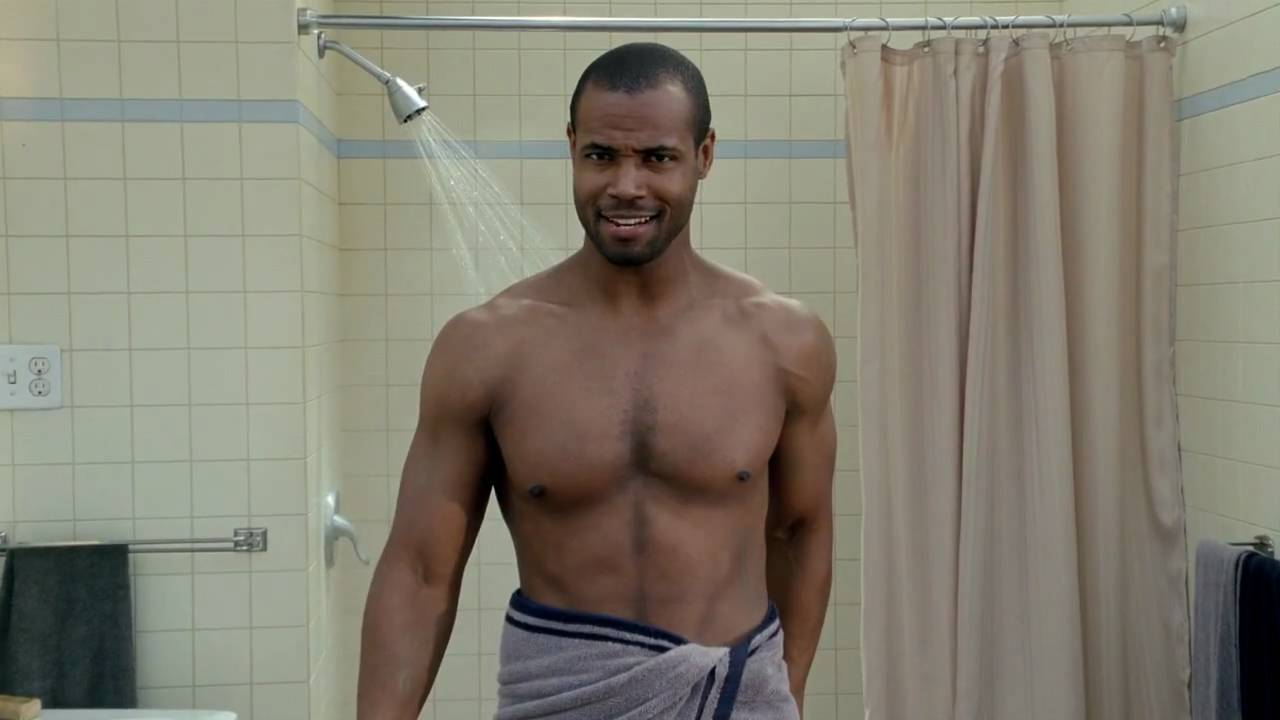
\includegraphics[width=1\textwidth,height=\textheight]{images/oldspice.jpg}
\caption{Old Spice: The Man Your Man Could Smell Like}
\end{figure}

In summary, a successful social media campaign is multifaceted, encompassing a clear understanding of objectives, audience, and the dynamic nature of social media platforms. By analyzing these elements and addressing the inherent challenges, future campaigns can be better equipped to navigate the complex landscape of social media marketing.

\hypertarget{data-collection-tools}{%
\chapter{Data Collection Tools}\label{data-collection-tools}}

\hypertarget{overview-of-analytics-tools}{%
\section*{Overview of Analytics Tools}\label{overview-of-analytics-tools}}
\addcontentsline{toc}{section}{Overview of Analytics Tools}

\hypertarget{introduction-to-analytics-tools}{%
\subsection*{Introduction to Analytics Tools}\label{introduction-to-analytics-tools}}
\addcontentsline{toc}{subsection}{Introduction to Analytics Tools}

In the realm of social media strategy, the deployment of analytics tools is not merely advantageous; it is essential. These tools furnish marketers, data analysts, and researchers with the capability to decipher vast amounts of data generated by social media platforms, transforming raw metrics into actionable insights. This transformation is crucial for understanding and enhancing user engagement, tailoring content to audience preferences, and measuring the efficacy of social media campaigns.

\hypertarget{importance-of-analytics-in-social-media-strategy}{%
\subsubsection*{Importance of Analytics in Social Media Strategy}\label{importance-of-analytics-in-social-media-strategy}}
\addcontentsline{toc}{subsubsection}{Importance of Analytics in Social Media Strategy}

Analytics tools serve as the cornerstone for informed decision-making in social media marketing. They allow for the tracking of key performance indicators (KPIs) such as likes, shares, comments, page views, and conversion rates. By analyzing these metrics, organizations can optimize their social media strategies to achieve specific objectives, whether they be increasing brand awareness, enhancing customer engagement, or driving sales. Moreover, analytics tools enable the identification of trends and patterns in user behavior, facilitating the prediction of future interactions and the tailoring of content to meet the evolving preferences of the target audience.

\hypertarget{role-in-understanding-user-engagement-and-behavior}{%
\subsubsection*{Role in Understanding User Engagement and Behavior}\label{role-in-understanding-user-engagement-and-behavior}}
\addcontentsline{toc}{subsubsection}{Role in Understanding User Engagement and Behavior}

Understanding user engagement and behavior is paramount in crafting a social media strategy that resonates with an audience. Analytics tools provide a window into the user's world, offering insights into what content performs well, the times users are most active, and the types of interactions that occur with the brand's social media presence. This understanding allows for the refinement of content strategies, ensuring that posts are both relevant and engaging to the audience. Furthermore, analytics can shed light on the customer journey, from initial contact through to conversion, highlighting opportunities to enhance the user experience and foster brand loyalty.

\hypertarget{overview-of-tool-capabilities-and-applications}{%
\subsubsection*{Overview of Tool Capabilities and Applications}\label{overview-of-tool-capabilities-and-applications}}
\addcontentsline{toc}{subsubsection}{Overview of Tool Capabilities and Applications}

The capabilities of analytics tools extend beyond mere data collection; they encompass a broad spectrum of functionalities designed to dissect and interpret social media data. These tools can track real-time interactions, segment audiences based on demographics or behavior, and measure the return on investment (ROI) of social media campaigns. Applications of these tools are varied and can range from simple tasks such as scheduling posts and monitoring hashtag performance to more complex analyses like sentiment analysis and predictive modeling.

For instance, R and RStudio, while not exclusively social media analytics tools, are powerful allies in the analysis and visualization of social media data. R, a programming language and software environment for statistical computing, coupled with RStudio, an integrated development environment (IDE) for R, enables researchers and analysts to perform sophisticated data analysis and create compelling visualizations. This combination is particularly useful for custom analyses that go beyond the capabilities of standard social media analytics tools, allowing for the exploration of user sentiment, trend analysis, and network analysis. Through packages designed specifically for social media data (like \texttt{twitteR} for Twitter data, \texttt{Rfacebook} for Facebook data, and others), users can collect, process, and analyze data in ways that are tailored to their specific research questions or business needs.

The strategic application of analytics tools, including the adept use of R and RStudio for custom data analysis, is indispensable in navigating the complex landscape of social media. These tools not only illuminate the path to enhanced engagement and strategic alignment but also empower organizations to leverage data-driven insights for competitive advantage.

\hypertarget{google-analytics}{%
\subsection*{Google Analytics}\label{google-analytics}}
\addcontentsline{toc}{subsection}{Google Analytics}

Google Analytics stands as a paramount tool in the domain of web analytics, offering extensive capabilities for tracking website traffic, analyzing user behavior, and integrating data from social media platforms. Its comprehensive suite of features enables organizations to glean actionable insights from their online presence, informing strategies that enhance user engagement and drive conversions. For social media analysts and marketers, Google Analytics provides a powerful means to measure the impact of social media on website traffic and to understand how users interact with their content across different channels.

\hypertarget{tracking-website-traffic-and-social-media-integration}{%
\subsubsection*{Tracking Website Traffic and Social Media Integration}\label{tracking-website-traffic-and-social-media-integration}}
\addcontentsline{toc}{subsubsection}{Tracking Website Traffic and Social Media Integration}

Google Analytics excels in its ability to track users' interactions with a website, offering detailed insights into the source of traffic, including direct visits, search engine referrals, and social media platforms. By integrating social media data, analysts can discern the effectiveness of social media campaigns in driving traffic to their website. This integration is crucial for understanding the role of social media within the broader digital marketing strategy, allowing organizations to attribute conversions and engagements directly to their social media efforts.

\textbf{Social Media Reporting}: Leveraging Google Analytics' social media reports, users can identify which platforms are generating the most traffic, the quality of this traffic in terms of engagement and conversion rates, and how users from different platforms behave once they land on the website.

\hypertarget{setting-up-and-interpreting-goals}{%
\subsubsection*{Setting Up and Interpreting Goals}\label{setting-up-and-interpreting-goals}}
\addcontentsline{toc}{subsubsection}{Setting Up and Interpreting Goals}

Goals in Google Analytics are used to track how well a website fulfills target objectives, such as form submissions, product purchases, or time spent on a page. Setting up goals allows marketers to measure conversions that originate from social media channels, providing a clear picture of social media ROI.

\textbf{Conversion Tracking}: By defining specific actions as goals, analysts can pinpoint which social media platforms contribute most to desired outcomes, enabling targeted strategy refinement.

\textbf{Funnel Analysis}: Through goal funnels, Google Analytics can show the path users take towards conversion, highlighting potential drop-off points and opportunities for optimization.

\hypertarget{audience-demographics-and-behavior-analysis}{%
\subsubsection*{Audience Demographics and Behavior Analysis}\label{audience-demographics-and-behavior-analysis}}
\addcontentsline{toc}{subsubsection}{Audience Demographics and Behavior Analysis}

Understanding who visits a website and how they interact with it is crucial for tailoring content and marketing strategies. Google Analytics offers in-depth analysis of audience demographics (age, gender, interests) and behavior (new vs.~returning users, frequency of visits, engagement metrics).

\textbf{Segmentation}: This feature allows for the segmentation of traffic from social media to analyze specific groups' behavior, providing insights into how different demographic segments interact with the website.

\textbf{Behavior Flow}: Visualizing the path users take through the site, from entry to exit, helps identify content that resonates with the audience, as well as potential obstacles in the user journey.

\hypertarget{utilizing-reports-for-social-media-strategy-refinement}{%
\subsubsection*{Utilizing Reports for Social Media Strategy Refinement}\label{utilizing-reports-for-social-media-strategy-refinement}}
\addcontentsline{toc}{subsubsection}{Utilizing Reports for Social Media Strategy Refinement}

The reports generated by Google Analytics are instrumental in refining social media strategies. By analyzing data on user interactions, conversions, and the effectiveness of different social media channels, organizations can make informed decisions about where to allocate resources and how to adjust their content and messaging for optimal engagement.

\textbf{Custom Reports}: Tailored reports can be created to focus on specific aspects of social media performance, offering customized insights that align with organizational goals.

\textbf{Integration with R \& RStudio}: For deeper analysis, data from Google Analytics can be exported and analyzed using R \& RStudio. This allows for the application of statistical models, trend analysis, and the creation of bespoke visualizations, providing a more nuanced understanding of the data.

Google Analytics offers a robust framework for tracking, analyzing, and optimizing the intersection of website traffic and social media engagement. When used in conjunction with advanced analytical tools like R \& RStudio, it enables a granular analysis of social media's impact on digital marketing objectives, empowering organizations to craft data-driven strategies that resonate with their audience and amplify their online presence.

\hypertarget{hootsuite}{%
\subsection*{Hootsuite}\label{hootsuite}}
\addcontentsline{toc}{subsection}{Hootsuite}

Hootsuite is a comprehensive social media management platform that empowers organizations and individuals to streamline their social media activities. From scheduling posts to monitoring conversations and analyzing performance metrics, Hootsuite provides a centralized dashboard for managing multiple social media accounts across various platforms. Its robust suite of tools is designed to enhance audience engagement, monitor brand reputation, and optimize social media strategies through data-driven insights.

\hypertarget{features-for-post-scheduling-and-social-media-monitoring}{%
\subsubsection*{Features for Post Scheduling and Social Media Monitoring}\label{features-for-post-scheduling-and-social-media-monitoring}}
\addcontentsline{toc}{subsubsection}{Features for Post Scheduling and Social Media Monitoring}

Hootsuite's post scheduling feature allows users to plan and publish content across different social media platforms from a single interface. This functionality not only saves time but also ensures that content reaches the audience at optimal times for engagement. In addition to scheduling, Hootsuite offers comprehensive monitoring capabilities, enabling users to track mentions, keywords, and trends in real-time. This is crucial for engaging with the audience promptly and managing brand reputation effectively.

\textbf{Streamlining Content Management}: Automating the posting process for consistency and efficiency.

\textbf{Real-time Engagement}: Monitoring social media feeds to respond quickly to user interactions, mentions, and direct messages.

\hypertarget{traffic-and-campaign-analysis-across-platforms}{%
\subsubsection*{Traffic and Campaign Analysis across Platforms}\label{traffic-and-campaign-analysis-across-platforms}}
\addcontentsline{toc}{subsubsection}{Traffic and Campaign Analysis across Platforms}

Hootsuite's analytics tools offer a detailed view of social media performance across platforms, enabling users to measure the impact of their campaigns and identify areas for improvement. By analyzing traffic, engagement rates, and conversion metrics, organizations can gauge the effectiveness of their social media strategies and make data-informed adjustments.

\textbf{Cross-Platform Analytics}: Aggregating data from various social media platforms to provide a unified view of social media performance.

\textbf{Campaign Tracking}: Monitoring specific campaigns to assess their reach, engagement, and overall success.

\hypertarget{utilizing-hootsuite-for-audience-engagement-and-brand-monitoring}{%
\subsubsection*{Utilizing Hootsuite for Audience Engagement and Brand Monitoring}\label{utilizing-hootsuite-for-audience-engagement-and-brand-monitoring}}
\addcontentsline{toc}{subsubsection}{Utilizing Hootsuite for Audience Engagement and Brand Monitoring}

Engaging with the audience and monitoring brand health are critical components of successful social media management. Hootsuite facilitates these processes by providing tools that help users listen to their audience and track sentiment regarding their brand. This proactive approach to engagement and monitoring helps in building a positive brand image and fostering a loyal community.

\textbf{Sentiment Analysis}: Gauging the mood and perceptions of the audience towards the brand or specific topics.

\textbf{Brand Health Monitoring}: Keeping tabs on brand mentions and sentiment to manage reputation and address potential issues promptly.

\hypertarget{reporting-and-analytics-capabilities}{%
\subsubsection*{Reporting and Analytics Capabilities}\label{reporting-and-analytics-capabilities}}
\addcontentsline{toc}{subsubsection}{Reporting and Analytics Capabilities}

Hootsuite's reporting and analytics capabilities are designed to transform social media data into actionable insights. Customizable reports allow users to focus on the metrics that matter most to their strategy, enabling the optimization of content and engagement tactics based on empirical evidence.

\textbf{Custom Reports}: Tailoring reports to highlight key performance indicators and trends relevant to organizational goals.

\textbf{Integration with R \& RStudio for Advanced Analysis}: For those requiring more in-depth analysis, Hootsuite's data can be exported and further analyzed using R \& RStudio. This allows for the application of statistical analysis, predictive modeling, and custom visualization to delve deeper into social media performance and user behavior.

Hootsuite stands out as a versatile tool for managing and optimizing social media activities. Its ability to schedule posts, monitor engagement, and analyze performance across platforms makes it an invaluable asset for social media marketers. When combined with the analytical power of R \& RStudio, Hootsuite's data can be leveraged for advanced analysis, offering deeper insights into social media strategy effectiveness and opportunities for refinement.

\hypertarget{buffer}{%
\subsection*{Buffer}\label{buffer}}
\addcontentsline{toc}{subsection}{Buffer}

Buffer is a highly regarded tool in the social media management space, known for its simplicity and effectiveness in scheduling posts, managing multiple accounts, and analyzing social media performance. It facilitates the planning and execution of social media strategies by offering a suite of features designed to optimize content distribution, engagement, and audience analysis. Buffer's analytics capabilities are instrumental for marketers and social media managers looking to refine their approach based on solid data insights.

\hypertarget{post-scheduling-and-management-for-multiple-accounts}{%
\subsubsection*{Post Scheduling and Management for Multiple Accounts}\label{post-scheduling-and-management-for-multiple-accounts}}
\addcontentsline{toc}{subsubsection}{Post Scheduling and Management for Multiple Accounts}

One of Buffer's core features is its ability to allow users to schedule posts across various social media platforms from a single dashboard. This streamlines the content management process, saving time and ensuring a consistent online presence. Moreover, Buffer supports the management of multiple accounts, making it easier for users to maintain a cohesive social media strategy across different channels and brands.

\textbf{Efficient Content Distribution}: Automating the scheduling of posts to ensure consistent content delivery at optimal times.

\textbf{Centralized Account Management}: Managing multiple social media accounts seamlessly from one platform.

\hypertarget{analyzing-engagement-trends-and-identifying-optimal-posting-times}{%
\subsubsection*{Analyzing Engagement Trends and Identifying Optimal Posting Times}\label{analyzing-engagement-trends-and-identifying-optimal-posting-times}}
\addcontentsline{toc}{subsubsection}{Analyzing Engagement Trends and Identifying Optimal Posting Times}

Buffer's analytics tools provide valuable insights into how content is performing on social media. By analyzing engagement trends, such as likes, shares, comments, and clicks, users can identify what content resonates most with their audience. Furthermore, Buffer offers data on optimal posting times, enabling users to schedule their content when it is most likely to be seen and engaged with by their target audience.

\textbf{Engagement Analysis}: Evaluating the performance of posts to understand what drives audience interaction.

\textbf{Optimal Timing Insights}: Leveraging data to determine the best times for posting to maximize visibility and engagement.

\hypertarget{understanding-audience-demographics-and-preferences}{%
\subsubsection*{Understanding Audience Demographics and Preferences}\label{understanding-audience-demographics-and-preferences}}
\addcontentsline{toc}{subsubsection}{Understanding Audience Demographics and Preferences}

Gaining a deep understanding of the audience is crucial for tailoring content and engagement strategies. Buffer helps in this regard by providing detailed insights into audience demographics and preferences. This information allows social media managers to create more targeted and relevant content that appeals to the specific interests and needs of their audience.

\textbf{Audience Segmentation}: Analyzing audience data to segment users based on demographics, interests, and behavior.

\textbf{Content Customization}: Using insights gained from audience analysis to inform content creation and curation.

\hypertarget{integrating-buffer-analytics-into-social-media-planning}{%
\subsubsection*{Integrating Buffer Analytics into Social Media Planning}\label{integrating-buffer-analytics-into-social-media-planning}}
\addcontentsline{toc}{subsubsection}{Integrating Buffer Analytics into Social Media Planning}

The insights gained from Buffer's analytics can be a goldmine for social media planning. By integrating these insights into the strategic planning process, organizations can make informed decisions about content creation, posting schedules, and engagement tactics. Buffer's analytics help in identifying successful content types and strategies, guiding the optimization of future social media efforts for better performance.

\textbf{Strategic Decision-Making}: Utilizing analytics to inform content strategy, campaign planning, and resource allocation.

\textbf{Advanced Analysis with R \& RStudio}: For deeper dives into social media data, Buffer's analytics can be exported and analyzed using R \& RStudio. This allows for sophisticated statistical analysis, trend detection, and the creation of custom visualizations to uncover deeper insights into social media performance and audience behavior.

Buffer stands out as an essential tool for managing and optimizing social media activities. Its strengths in post scheduling, engagement analysis, audience insights, and strategic integration make it a valuable asset for anyone looking to enhance their social media presence. When combined with the analytical capabilities of R \& RStudio, Buffer's data can provide even more nuanced insights, empowering users to craft data-driven, effective social media strategies.

\hypertarget{comparative-analysis-1}{%
\subsection*{Comparative Analysis}\label{comparative-analysis-1}}
\addcontentsline{toc}{subsection}{Comparative Analysis}

In the landscape of social media analytics tools, choosing the right platform can be a daunting task given the variety of options available, each with its unique set of features, strengths, and limitations. A comparative analysis of prominent tools like Google Analytics, Hootsuite, Buffer, and the integration of R \& RStudio provides valuable insights into how these tools can be leveraged to meet organizational goals. This section aims to dissect these aspects to aid in the decision-making process, ensuring that organizations select the most appropriate tools for their specific needs.

\hypertarget{comparing-features-strengths-and-limitations}{%
\subsubsection*{Comparing Features, Strengths, and Limitations}\label{comparing-features-strengths-and-limitations}}
\addcontentsline{toc}{subsubsection}{Comparing Features, Strengths, and Limitations}

\textbf{Google Analytics} excels in providing detailed insights into website traffic and user behavior, including the impact of social media referrals. Its strengths lie in its comprehensive tracking capabilities, robust reporting, and ability to analyze audience demographics and behavior. However, its focus is more on website analytics rather than direct social media engagement or content management.

\textbf{Hootsuite} offers a wide array of features for managing social media accounts, including post scheduling, real-time monitoring, and engagement tools. It stands out for its dashboard that consolidates multiple social media platforms, allowing for efficient management and analytics across channels. Its limitations may include a learning curve for new users and the potential need for additional integrations for deeper analytics.

\textbf{Buffer} focuses on simplifying social media scheduling and analytics, providing users with intuitive tools for content planning and performance analysis. It is particularly strong in user-friendly scheduling features and straightforward analytics. However, it may not offer the depth of analytics or the comprehensive platform coverage seen in more specialized tools.

\textbf{R \& RStudio}, while not a direct social media management tool, offer unparalleled customization and depth in data analysis. Their strengths lie in the ability to conduct sophisticated statistical analyses, create custom visualizations, and handle large datasets. The primary limitation is the requirement of programming knowledge, which may present a barrier to entry for those unfamiliar with R.

\hypertarget{decision-making-criteria-for-tool-selection}{%
\subsubsection*{Decision-making Criteria for Tool Selection}\label{decision-making-criteria-for-tool-selection}}
\addcontentsline{toc}{subsubsection}{Decision-making Criteria for Tool Selection}

Selecting the right tool(s) hinges on several criteria:

\textbf{Organizational Objectives}: Whether the focus is on enhancing engagement, driving website traffic, or analyzing user behavior will influence tool choice.

\textbf{Technical Expertise}: The in-house team's familiarity with analytics tools and programming languages like R can determine the feasibility of using more complex platforms.

\textbf{Integration Needs}: The ability of the tool to integrate with existing systems and platforms used by the organization.

\textbf{Feature Requirements}: Prioritizing features such as real-time monitoring, detailed reporting, or predictive analytics based on strategic needs.

\hypertarget{customization-and-scalability-of-tools}{%
\subsubsection*{Customization and Scalability of Tools}\label{customization-and-scalability-of-tools}}
\addcontentsline{toc}{subsubsection}{Customization and Scalability of Tools}

The ability to customize and scale the tool according to changing business needs is crucial. R \& RStudio offer the highest level of customization through programming, allowing for tailored analyses and visualizations. Tools like Hootsuite and Buffer provide scalability through various subscription plans, but customization in terms of analytics may be limited compared to the flexibility R provides.

\hypertarget{cost-benefit-analysis-for-different-organizational-needs}{%
\subsubsection*{Cost-benefit Analysis for Different Organizational Needs}\label{cost-benefit-analysis-for-different-organizational-needs}}
\addcontentsline{toc}{subsubsection}{Cost-benefit Analysis for Different Organizational Needs}

Evaluating the cost against the potential benefits of each tool is essential for making an informed decision. While Google Analytics provides a robust set of features for free, advanced features may require a subscription. Hootsuite and Buffer offer tiered pricing plans, catering to different sizes of businesses and their specific needs. R \& RStudio, being open-source, present a cost-effective option for data analysis, with the primary investment being in the development of expertise to use them effectively.

The selection of social media analytics tools requires a careful consideration of the organization's specific goals, technical capabilities, and budget constraints. By understanding the unique features, strengths, and limitations of each tool, as well as their customization potential and scalability, organizations can make an informed choice that aligns with their strategic objectives and resource availability. The integration of advanced data analysis tools like R \& RStudio can further enhance the depth and breadth of insights, offering a competitive edge in the ever-evolving social media landscape.

\hypertarget{methods-for-data-collection}{%
\section*{Methods for Data Collection}\label{methods-for-data-collection}}
\addcontentsline{toc}{section}{Methods for Data Collection}

\hypertarget{understanding-apis}{%
\subsection*{Understanding APIs}\label{understanding-apis}}
\addcontentsline{toc}{subsection}{Understanding APIs}

Application Programming Interfaces (APIs) are fundamental to the ecosystem of social media data collection, serving as conduits through which data can be systematically accessed and retrieved from social media platforms. APIs allow for the efficient collection of large volumes of data, facilitating the analysis of user interactions, engagement patterns, and trending content. This section delves into the role of APIs in social media analytics, provides an overview of APIs from major platforms, and discusses the inherent limitations and possibilities they present.

\hypertarget{role-of-apis-in-social-media-data-collection}{%
\subsubsection*{Role of APIs in Social Media Data Collection}\label{role-of-apis-in-social-media-data-collection}}
\addcontentsline{toc}{subsubsection}{Role of APIs in Social Media Data Collection}

APIs play a pivotal role in enabling researchers, marketers, and analysts to gather data from social media platforms. They provide structured access to social media data, allowing for the retrieval of information such as user posts, comments, likes, and follower counts. This access is crucial for performing sentiment analysis, trend tracking, and understanding audience demographics. APIs thus serve as the backbone for many social media analytics tools, enabling them to offer users insights into the performance of their content and strategies.

\textbf{Automated Data Retrieval}: APIs facilitate the automated collection of social media data, enabling efficient and systematic data gathering processes.

\textbf{Real-time Analysis}: Many APIs allow for the collection of real-time data, making it possible to monitor current trends and user reactions as they happen.

\hypertarget{overview-of-major-social-media-platforms-apis}{%
\subsubsection*{Overview of Major Social Media Platforms' APIs}\label{overview-of-major-social-media-platforms-apis}}
\addcontentsline{toc}{subsubsection}{Overview of Major Social Media Platforms' APIs}

Each major social media platform offers its own API, each with unique functionalities and data access levels.

\textbf{Twitter API}: Offers extensive access to tweet data, user profiles, and engagement metrics. It is widely used for trend analysis, sentiment analysis, and monitoring public opinion.

\textbf{Facebook Graph API}: Allows access to a broad range of data on Facebook, including user posts, comments, and page analytics. It is crucial for understanding audience engagement on Facebook pages and profiles.

\textbf{Instagram Graph API}: Provides insights into Instagram business and creator accounts, including post performance, audience data, and story analytics. It supports content planning and performance analysis on Instagram.

\textbf{LinkedIn API}: Offers access to data on professional networking activities, including user profiles, connections, and interactions. It is valuable for B2B marketing and professional brand analysis.

\hypertarget{limitations-and-possibilities-of-api-data-collection}{%
\subsubsection*{Limitations and Possibilities of API Data Collection}\label{limitations-and-possibilities-of-api-data-collection}}
\addcontentsline{toc}{subsubsection}{Limitations and Possibilities of API Data Collection}

While APIs offer significant advantages for social media data collection, they come with limitations that researchers and analysts must navigate.

\textbf{Rate Limiting and Data Caps}: Most social media platforms impose limits on the number of requests that can be made to their APIs within a certain timeframe, potentially restricting the volume of data that can be collected.

\textbf{Access Restrictions}: Access to certain types of data may be restricted based on privacy policies and user settings, limiting the completeness of data collection.

\textbf{Data Complexity}: The data retrieved through APIs can be complex and require significant processing and analysis to derive meaningful insights.

However, the possibilities offered by API data collection are vast. With the right tools and techniques, such as those provided by R \& RStudio, analysts can overcome some of these limitations by efficiently processing and analyzing large datasets, extracting trends, and deriving insights that inform strategic decision-making. The use of R, in particular, allows for the customization of data collection and analysis processes, enabling researchers to tailor their approaches to meet specific research questions and organizational needs.

Understanding the role, capabilities, and limitations of social media APIs is crucial for effective social media data collection. Despite the challenges, the strategic use of APIs in conjunction with powerful analytical tools like R \& RStudio can unlock a wealth of insights into social media behavior and trends, providing a solid foundation for data-driven decision-making in social media strategy.

\hypertarget{api-usage-in-practice}{%
\subsection*{API Usage in Practice}\label{api-usage-in-practice}}
\addcontentsline{toc}{subsection}{API Usage in Practice}

Practical engagement with Application Programming Interfaces (APIs) is a cornerstone activity in the domain of social media analytics. This involves a series of steps from obtaining the necessary access and permissions to efficiently managing data quotas and structuring the data for analysis. The dynamic nature of social media platforms and the vast volume of data generated require a nuanced approach to API usage. This section outlines the practical aspects of utilizing APIs for social media data collection, focusing on the challenges and strategies involved in accessing and managing data.

\hypertarget{obtaining-access-and-permissions}{%
\subsubsection*{Obtaining Access and Permissions}\label{obtaining-access-and-permissions}}
\addcontentsline{toc}{subsubsection}{Obtaining Access and Permissions}

Access to social media APIs is typically controlled through an application process, where developers or researchers must register their project and obtain API keys or access tokens. This process is designed to protect user data and ensure that access is granted for legitimate purposes.

\textbf{Registration}: Users must create an account on the social media platform's developer portal and register their application, detailing its purpose and scope.

\textbf{API Keys and Access Tokens}: Upon approval, the platform issues API keys or access tokens, which are used to authenticate requests to the API.

\textbf{Permissions and Scopes}: Access to different types of data may require specific permissions, which need to be explicitly requested. The scope of access granted can vary significantly depending on the platform's policies and the nature of the application.

\hypertarget{navigating-rate-limits-and-data-quotas}{%
\subsubsection*{Navigating Rate Limits and Data Quotas}\label{navigating-rate-limits-and-data-quotas}}
\addcontentsline{toc}{subsubsection}{Navigating Rate Limits and Data Quotas}

Social media platforms impose rate limits and data quotas to manage the load on their servers and protect user data. These restrictions can significantly impact the scope and speed of data collection efforts.

\textbf{Understanding Rate Limits}: Rate limits specify the number of API requests that can be made within a given timeframe. Exceeding these limits can result in temporary blocks or suspension of API access.

\textbf{Managing Data Quotas}: Data quotas limit the volume of data that can be retrieved through the API. It is essential to plan data collection activities to stay within these quotas.

\textbf{Strategies for Efficient Data Collection}: Implementing strategies such as caching responses, staggering requests, and using webhooks (if available) can help mitigate the impact of rate limits and data quotas.

\hypertarget{working-with-api-responses-and-data-structuring}{%
\subsubsection*{Working with API Responses and Data Structuring}\label{working-with-api-responses-and-data-structuring}}
\addcontentsline{toc}{subsubsection}{Working with API Responses and Data Structuring}

The data retrieved through social media APIs typically comes in a structured format, such as JSON or XML, which requires parsing and processing to extract meaningful information.

\textbf{Parsing API Responses}: Tools and libraries in R, such as \texttt{jsonlite} for JSON data, can be used to parse API responses and convert them into a more manageable format for analysis.

\textbf{Data Structuring}: Once parsed, the data needs to be structured into a format suitable for analysis. This may involve transforming the data into data frames, filtering irrelevant information, and aggregating data points for higher-level analysis.

\textbf{Dealing with Complexity}: Social media data can be complex, with nested structures and linked objects. Understanding the data model of the social media platform's API is crucial for effective data structuring and analysis.

Integrating R and RStudio into the workflow for API data collection enhances the capability to handle large datasets, apply complex transformations, and perform sophisticated analyses. R's comprehensive ecosystem of packages and RStudio's user-friendly interface support a range of activities from data collection to visualization and reporting. By mastering the practical aspects of API usage, including obtaining access, navigating rate limits, and structuring data, analysts and researchers can unlock the full potential of social media data to inform strategic decisions and uncover insights into digital behaviors and trends.

\hypertarget{web-scraping-techniques}{%
\subsection*{Web Scraping Techniques}\label{web-scraping-techniques}}
\addcontentsline{toc}{subsection}{Web Scraping Techniques}

Web scraping is a powerful technique for extracting data from websites and social media platforms, serving as a complement or alternative to API-based data collection. Unlike APIs, which provide data in a structured format based on predefined access rules, web scraping involves programmatically navigating and extracting data from the HTML of web pages. This section explores the fundamentals of web scraping, the tools and languages that facilitate effective data extraction, and the ethical and legal considerations that govern its use.

\hypertarget{introduction-to-web-scraping-vs.-api-use}{%
\subsubsection*{Introduction to Web Scraping vs.~API Use}\label{introduction-to-web-scraping-vs.-api-use}}
\addcontentsline{toc}{subsubsection}{Introduction to Web Scraping vs.~API Use}

Web scraping and API use are two primary methods for collecting data from the web and social media platforms. While APIs offer a direct route to data provided by the platform, subject to rate limits and access permissions, web scraping allows for more flexible data collection by extracting information directly from the webpage.

\textbf{Flexibility and Control}: Web scraping provides flexibility in data collection, allowing for the extraction of data that may not be available through APIs.

\textbf{Data Availability}: APIs provide structured, reliable data access within the platform's limitations. In contrast, web scraping can access any publicly visible information, though it requires parsing and structuring the data post-collection.

\hypertarget{tools-and-languages-for-effective-scraping}{%
\subsubsection*{Tools and Languages for Effective Scraping}\label{tools-and-languages-for-effective-scraping}}
\addcontentsline{toc}{subsubsection}{Tools and Languages for Effective Scraping}

Several tools and programming languages support web scraping, with Python and R being among the most popular due to their libraries and frameworks designed for this purpose.

\textbf{Python}: Libraries such as BeautifulSoup and Scrapy are widely used for web scraping, offering robust features for HTML parsing and data extraction.

\textbf{R}: The \texttt{rvest} package in R simplifies web scraping by providing functions to read and manipulate web page contents. Combined with RStudio, it offers a comprehensive environment for data collection, processing, and analysis.

\hypertarget{ethical-and-legal-considerations-in-web-scraping}{%
\subsubsection*{Ethical and Legal Considerations in Web Scraping}\label{ethical-and-legal-considerations-in-web-scraping}}
\addcontentsline{toc}{subsubsection}{Ethical and Legal Considerations in Web Scraping}

Web scraping operates in a complex ethical and legal landscape, necessitating careful consideration of the sources from which data is collected.

\textbf{Respecting \texttt{robots.txt}}: Websites use \texttt{robots.txt} files to define rules about what parts of the site can be accessed by automated agents. Ethical web scraping involves adhering to these rules.

\textbf{Legal Restrictions}: The legality of web scraping varies by jurisdiction and specific website terms of service. It is crucial to review and comply with these terms and applicable laws, such as the Computer Fraud and Abuse Act (CFAA) in the United States.

\textbf{Privacy Concerns}: Collecting data from public websites must be balanced with respect for individual privacy, especially when dealing with personal or sensitive information.

\hypertarget{overcoming-technical-challenges-in-scraping-activities}{%
\subsubsection*{Overcoming Technical Challenges in Scraping Activities}\label{overcoming-technical-challenges-in-scraping-activities}}
\addcontentsline{toc}{subsubsection}{Overcoming Technical Challenges in Scraping Activities}

Web scraping presents several technical challenges, from navigating complex website structures to handling dynamic content loaded via JavaScript.

\textbf{Dynamic Content}: Many modern websites use JavaScript to load content dynamically, which can be challenging to scrape using traditional methods. Tools like Selenium or R's \texttt{RSelenium} package can automate web browsers to interact with dynamic content.

\textbf{Data Structuring}: Extracted data often requires significant cleaning and structuring to be useful for analysis. R provides a suite of tools for data manipulation and cleaning, such as \texttt{dplyr} and \texttt{tidyr}, which are essential for preparing scraped data.

\textbf{Rate Limiting and IP Blocking}: Websites may limit the rate of requests or block IP addresses that make too many rapid requests. Implementing delays between requests and using proxy servers can help mitigate these issues.

Web scraping, when done responsibly and legally, is an invaluable technique for data collection, offering access to a wide range of data that may not be accessible through official APIs. The integration of web scraping methodologies with R \& RStudio enhances the capacity for in-depth analysis, providing researchers and analysts with the tools necessary to extract, process, and analyze web data effectively. However, it is imperative to navigate the ethical and legal considerations carefully to ensure that web scraping practices respect the rights of data owners and comply with legal standards.

\hypertarget{real-time-data-collection}{%
\subsection*{Real-time Data Collection}\label{real-time-data-collection}}
\addcontentsline{toc}{subsection}{Real-time Data Collection}

In the fast-paced environment of social media, real-time data collection is crucial for capturing the dynamics of user interactions, trending topics, and emerging narratives as they unfold. This capability enables organizations and researchers to react promptly to online conversations, adjust strategies in response to live events, and leverage trending moments for enhanced engagement. This section outlines the importance and applications of real-time data, explores tools and technologies for live data collection, and discusses strategies for analyzing and responding to trends as they develop.

\hypertarget{importance-and-applications-of-real-time-data}{%
\subsubsection*{Importance and Applications of Real-time Data}\label{importance-and-applications-of-real-time-data}}
\addcontentsline{toc}{subsubsection}{Importance and Applications of Real-time Data}

Real-time data collection from social media platforms offers immediate insights into public opinion, user behavior, and content performance, providing a competitive edge in both academic research and strategic marketing.

\textbf{Crisis Monitoring and Management}: Real-time data allows for the quick detection of potential crises or negative sentiment, enabling timely responses to mitigate potential damage.

\textbf{Event and Campaign Tracking}: Live data collection supports the monitoring of social media activities related to specific events or marketing campaigns, facilitating adjustments to optimize engagement and reach.

\textbf{Trend Discovery}: Identifying and engaging with trending topics in real-time can significantly increase visibility and audience engagement.

\hypertarget{tools-and-technologies-for-live-data-collection}{%
\subsubsection*{Tools and Technologies for Live Data Collection}\label{tools-and-technologies-for-live-data-collection}}
\addcontentsline{toc}{subsubsection}{Tools and Technologies for Live Data Collection}

Several tools and technologies are specifically designed to facilitate the real-time collection and analysis of social media data, with some offering integration capabilities with R \& RStudio for advanced analytics.

\textbf{Social Media APIs}: Many social media platforms offer streaming APIs that provide real-time access to public posts, tweets, and interactions. For instance, the Twitter Streaming API allows for the collection of tweets as they are posted.

\textbf{Third-party Tools}: Platforms like DataSift and Gnip provide access to real-time social media data streams, offering aggregated data across multiple social media platforms.

\textbf{R Packages}: Packages such as \texttt{streamR} for R provide interfaces to streaming APIs, enabling the collection and analysis of live data directly within the R environment.

\hypertarget{analyzing-and-responding-to-trends-in-real-time}{%
\subsubsection*{Analyzing and Responding to Trends in Real-time}\label{analyzing-and-responding-to-trends-in-real-time}}
\addcontentsline{toc}{subsubsection}{Analyzing and Responding to Trends in Real-time}

The ability to analyze and respond to real-time data requires a combination of automated data collection, rapid analysis techniques, and strategic planning to leverage insights effectively.

\textbf{Automated Monitoring and Alerts}: Setting up automated systems to monitor for specific keywords, hashtags, or sentiment can help in identifying trends as they emerge. Tools like \texttt{Shiny} in R can be used to create interactive, real-time dashboards for data visualization and monitoring.

\textbf{Rapid Analysis Techniques}: Utilizing R's capabilities for text analysis, sentiment analysis, and statistical modeling enables quick interpretation of real-time data. This can inform immediate strategic decisions, from content adjustment to crisis response.

\textbf{Engagement Strategies}: Based on real-time analytics, organizations can develop responsive engagement strategies, such as participating in trending conversations, adjusting ad spend, or publishing content aligned with current trends.

Real-time data collection and analysis offer invaluable insights into the ever-changing landscape of social media, providing the means to engage with audiences more effectively and make informed decisions based on live data. Integrating these practices with the analytical power of R \& RStudio enhances the ability to dissect large volumes of real-time data, uncover patterns, and respond to social media dynamics with precision and agility. By leveraging these tools and technologies, researchers and practitioners can stay at the forefront of social media trends, maximizing impact and engagement in an increasingly connected world.

\hypertarget{data-collection-challenges}{%
\subsection*{Data Collection Challenges}\label{data-collection-challenges}}
\addcontentsline{toc}{subsection}{Data Collection Challenges}

Collecting data from social media platforms, while rich in potential insights, presents a myriad of challenges ranging from managing vast and complex datasets to navigating the evolving landscape of platform policies and technical limitations. This section delves into the common hurdles encountered in social media data collection, specifically focusing on handling large and unstructured datasets, adapting to platform API changes and restrictions, and ensuring the quality and relevance of the data collected. It also offers strategies for overcoming these challenges, leveraging the capabilities of R \& RStudio to facilitate robust and efficient data collection processes.

\hypertarget{handling-large-and-unstructured-datasets}{%
\subsubsection*{Handling Large and Unstructured Datasets}\label{handling-large-and-unstructured-datasets}}
\addcontentsline{toc}{subsubsection}{Handling Large and Unstructured Datasets}

Social media platforms generate immense volumes of data daily, characterized by their unstructured nature, including text, images, videos, and user interactions. Managing and analyzing such datasets require sophisticated tools and techniques.

\textbf{Big Data Technologies}: Integrating R with big data technologies like Apache Hadoop or Spark can help process and analyze large datasets. Packages such as \texttt{sparklyr} offer a seamless interface between R and Spark, allowing for the distributed processing of large datasets.

\textbf{Data Structuring and Cleaning}: Utilizing R packages like \texttt{tidyr} for tidying data and \texttt{dplyr} for data manipulation can significantly streamline the process of structuring and cleaning unstructured datasets, making them more amenable to analysis.

\hypertarget{adapting-to-platform-api-changes-and-restrictions}{%
\subsubsection*{Adapting to Platform API Changes and Restrictions}\label{adapting-to-platform-api-changes-and-restrictions}}
\addcontentsline{toc}{subsubsection}{Adapting to Platform API Changes and Restrictions}

Social media platforms frequently update their APIs and impose new restrictions on data access, posing significant challenges to data collection efforts. These changes can affect the scope of data available and the methods used for collection.

\textbf{Staying Informed}: Regularly monitoring platform developer blogs and API documentation is crucial for staying up-to-date with changes.

\textbf{Flexible Data Collection Frameworks}: Developing flexible data collection scripts in R that can be easily modified to accommodate API changes. Utilizing abstraction layers or wrapper packages in R, such as \texttt{httr} for handling HTTP requests, can simplify the process of adapting to API changes.

\hypertarget{ensuring-data-quality-and-relevance}{%
\subsubsection*{Ensuring Data Quality and Relevance}\label{ensuring-data-quality-and-relevance}}
\addcontentsline{toc}{subsubsection}{Ensuring Data Quality and Relevance}

The quality and relevance of collected data are paramount for meaningful social media analysis. Challenges include filtering out irrelevant content, verifying the authenticity of data, and addressing biases.

\textbf{Data Filtering and Preprocessing}: Implementing robust data filtering mechanisms using R to remove irrelevant or redundant information. Packages such as \texttt{stringr} for string manipulation and \texttt{lubridate} for date/time operations are essential for preprocessing tasks.

\textbf{Addressing Biases}: Identifying and mitigating biases in data collection is critical for ensuring the representativeness of the dataset. Techniques such as stratified sampling can be applied using R to ensure diverse and representative data collection.

\textbf{Verification and Validation}: Employing techniques to verify the authenticity of the data and validate its relevance to the research questions or business objectives. This may include sentiment analysis using packages like \texttt{syuzhet} or \texttt{tm} for text mining to assess the sentiment and thematic relevance of the data.

Overcoming these challenges requires a combination of staying informed about the latest platform developments, employing flexible and robust data collection frameworks, and applying rigorous data processing and analysis techniques. The versatility of R \& RStudio, through its vast ecosystem of packages and its capability for integration with other technologies, provides a powerful platform for navigating the complexities of social media data collection. By leveraging these tools, researchers and practitioners can enhance the efficiency, accuracy, and relevance of their social media analytics efforts, unlocking deeper insights and driving more informed decisions.

\hypertarget{ethical-considerations-in-data-collection}{%
\section*{Ethical Considerations in Data Collection}\label{ethical-considerations-in-data-collection}}
\addcontentsline{toc}{section}{Ethical Considerations in Data Collection}

In the domain of social media analytics, ethical considerations play a pivotal role in guiding how data is collected, analyzed, and utilized. The vast amount of personal and sensitive information available through social media platforms necessitates a rigorous ethical framework to protect individuals' privacy and ensure the responsible use of data. This section outlines essential ethical guidelines for social media data collection, emphasizing the importance of respecting user privacy, maintaining transparency in data collection and analysis methods, and ensuring the ethical use of analytics tools and data.

\hypertarget{ethical-guidelines}{%
\subsection*{Ethical Guidelines}\label{ethical-guidelines}}
\addcontentsline{toc}{subsection}{Ethical Guidelines}

\hypertarget{respecting-user-privacy-and-platform-policies}{%
\subsubsection*{Respecting User Privacy and Platform Policies}\label{respecting-user-privacy-and-platform-policies}}
\addcontentsline{toc}{subsubsection}{Respecting User Privacy and Platform Policies}

User privacy is a cornerstone of ethical data collection practices. Researchers and analysts must navigate the delicate balance between collecting data for insightful analysis and respecting individuals' rights to privacy.

\textbf{Informed Consent}: Whenever possible, obtaining informed consent from users whose data is being collected is paramount. This may not always be feasible in large-scale data collection; however, efforts should be made to ensure data collection does not infringe on individual privacy rights.

\textbf{Adhering to Platform Policies}: Social media platforms have their own set of terms of service and data use policies. Compliance with these policies is mandatory to respect the platforms' rules and the privacy of their users. Researchers should familiarize themselves with these policies to ensure their data collection methods are in alignment.

\hypertarget{transparency-in-data-collection-and-analysis-methods}{%
\subsubsection*{Transparency in Data Collection and Analysis Methods}\label{transparency-in-data-collection-and-analysis-methods}}
\addcontentsline{toc}{subsubsection}{Transparency in Data Collection and Analysis Methods}

Transparency about how data is collected, processed, and analyzed is critical for maintaining the trust and integrity of social media research.

\textbf{Disclosure}: Clearly disclosing the methodologies used for data collection and analysis helps build trust with the public and the research community. This includes detailing the tools, algorithms, and analytical methods employed in the study.

\textbf{Openness}: Where possible, sharing the results of analyses and the implications of findings in an open and accessible manner contributes to the collective knowledge base and fosters an environment of transparency.

\hypertarget{ethical-use-of-analytics-tools-and-data}{%
\subsubsection*{Ethical Use of Analytics Tools and Data}\label{ethical-use-of-analytics-tools-and-data}}
\addcontentsline{toc}{subsubsection}{Ethical Use of Analytics Tools and Data}

The ethical implications of using analytics tools and the data collected through them extend beyond privacy concerns and transparency. It encompasses the broader responsibility of using data in a manner that is respectful, non-discriminatory, and beneficial.

\textbf{Non-Discrimination}: Ensuring that data collection and analysis methods do not inadvertently reinforce biases or lead to discriminatory practices. This involves being mindful of algorithmic biases that may skew results and impact certain groups disproportionately.

\textbf{Beneficence}: Striving to ensure that the outcomes of data analysis contribute positively to society, whether by enhancing understanding of social dynamics, improving technological solutions, or informing policy.

\textbf{Accountability}: Taking responsibility for the ethical implications of data analysis and being prepared to address any negative impacts that may arise from the research.

Incorporating R \& RStudio into the ethical framework for social media data collection enhances the ability to adhere to these guidelines through the use of packages and functions designed with privacy and transparency in mind. For example, using R Markdown can aid in creating transparent and reproducible analysis documents, while specialized packages can assist in anonymizing datasets before analysis.

Ultimately, ethical considerations in social media data collection and analysis are not just a set of obligations but a foundational component of responsible research and analytics practices. By adhering to these ethical guidelines, researchers and practitioners not only protect individuals' rights and privacy but also enhance the credibility and utility of their work in the field of social media analytics.

\hypertarget{informed-consent}{%
\subsection*{Informed Consent}\label{informed-consent}}
\addcontentsline{toc}{subsection}{Informed Consent}

Informed consent represents a fundamental ethical principle in the realm of social media research, ensuring that individuals are aware of and agree to the collection and use of data derived from their online activities. This section explores the critical role of informed consent in social media research, outlines various methods for obtaining consent, and discusses the unique challenges and considerations that arise in digital environments.

\hypertarget{importance-in-social-media-research}{%
\subsubsection*{Importance in Social Media Research}\label{importance-in-social-media-research}}
\addcontentsline{toc}{subsubsection}{Importance in Social Media Research}

Informed consent is crucial for respecting individual autonomy and privacy in social media research. It serves several key purposes:

\textbf{Respect for Autonomy}: It acknowledges and respects an individual's right to control their personal information and to make informed decisions about their participation in research.

\textbf{Protection of Privacy}: It helps protect the privacy of individuals by ensuring that they are aware of what data is being collected, how it will be used, and whom it will be shared with.

\textbf{Ethical Integrity}: It upholds the ethical integrity of the research process by ensuring that participants are not deceived or coerced into providing data.

\hypertarget{methods-for-obtaining-consent}{%
\subsubsection*{Methods for Obtaining Consent}\label{methods-for-obtaining-consent}}
\addcontentsline{toc}{subsubsection}{Methods for Obtaining Consent}

Obtaining informed consent in social media research can be challenging, especially when dealing with large datasets or public data. However, several methods can be employed to address these challenges:

\textbf{Direct Consent}: For small-scale studies or when interacting directly with participants, researchers can obtain consent through direct communication, such as emails, direct messages, or online consent forms.

\textbf{Terms of Service Agreements}: When using social media platforms for data collection, researchers may rely on the platform's terms of service, which users agree to upon creating an account. However, this approach should be supplemented with efforts to ensure that users are genuinely informed about the research use of their data.

\textbf{Public Data Considerations}: For data that is publicly available, researchers should consider the nature of the consent implied by users making their data public and the expectations of privacy that users may have.

\hypertarget{challenges-and-considerations-in-digital-environments}{%
\subsubsection*{Challenges and Considerations in Digital Environments}\label{challenges-and-considerations-in-digital-environments}}
\addcontentsline{toc}{subsubsection}{Challenges and Considerations in Digital Environments}

Digital environments present unique challenges for obtaining informed consent, necessitating careful consideration of the following aspects:

\textbf{Anonymity and Privacy}: In cases where data is collected from public forums or social media platforms, maintaining the anonymity and privacy of individuals is paramount. Researchers must navigate the fine line between public and private data, recognizing that publicly posted information may still carry expectations of privacy.

\textbf{Dynamic Consent}: The dynamic nature of digital platforms, where users can change their privacy settings or delete content, requires researchers to consider the ongoing consent of participants. Researchers must be prepared to respect changes in users' consent status.

\textbf{Transparency and Comprehension}: Ensuring that consent processes are transparent and that information is presented in a manner that is easily understood by all participants is critical. This includes clear communication about the scope of data collection, the purposes of the research, and any potential risks involved.

Utilizing tools and methodologies that respect informed consent principles is essential in social media research. R \& RStudio can support ethical practices through the development of tools for anonymizing data, analyzing public datasets responsibly, and documenting the consent process in research workflows. By prioritizing informed consent, researchers can navigate the ethical complexities of social media data collection, fostering trust and integrity in their work.

\hypertarget{data-anonymization-and-privacy}{%
\subsection*{Data Anonymization and Privacy}\label{data-anonymization-and-privacy}}
\addcontentsline{toc}{subsection}{Data Anonymization and Privacy}

In the context of social media analytics, safeguarding individuals' privacy through data anonymization is a critical ethical and legal obligation. Anonymization involves altering personal data in such a way that the individual cannot be identified, either directly or indirectly, thereby protecting their privacy while allowing for valuable insights to be gleaned from the data. This section discusses various techniques for anonymizing collected data, outlines the importance of compliance with legal frameworks such as the GDPR (General Data Protection Regulation) and the CCPA (California Consumer Privacy Act), and highlights the ethical considerations in handling sensitive information.

\hypertarget{techniques-for-anonymizing-collected-data}{%
\subsubsection*{Techniques for Anonymizing Collected Data}\label{techniques-for-anonymizing-collected-data}}
\addcontentsline{toc}{subsubsection}{Techniques for Anonymizing Collected Data}

Effective data anonymization ensures that privacy is maintained without significantly diminishing the utility of the data for analysis. Techniques include:

\textbf{Data Masking}: Replacing identifiable information with fictional but plausible data. This can maintain the utility of the data set for analysis while protecting individual identities.

\textbf{Pseudonymization}: Replacing private identifiers with pseudonyms or codes, which can be particularly useful in longitudinal studies where tracking individual responses over time is necessary without revealing their identities.

\textbf{Aggregation}: Summarizing data at a higher level, such as by demographic group or geographical area, to prevent the identification of individuals from the data.

\textbf{Randomization}: Introducing noise into the data set to obscure the original data points while preserving the overall distribution and relationships within the data.

In R, packages such as \texttt{sdcMicro} can be used for anonymizing data by applying various statistical disclosure control techniques, ensuring that the privacy of individuals is protected while maintaining the integrity of the data for analysis.

\hypertarget{compliance-with-legal-frameworks-gdpr-ccpa}{%
\subsubsection*{Compliance with Legal Frameworks (GDPR, CCPA)}\label{compliance-with-legal-frameworks-gdpr-ccpa}}
\addcontentsline{toc}{subsubsection}{Compliance with Legal Frameworks (GDPR, CCPA)}

Compliance with data protection regulations is not only a legal requirement but also a demonstration of commitment to ethical practices in data collection and analysis.

\textbf{General Data Protection Regulation (GDPR)}: Enacted by the European Union, the GDPR imposes strict rules on data privacy and protection, including requirements for data minimization, purpose limitation, and the rights of individuals to have their data erased.

\textbf{California Consumer Privacy Act (CCPA)}: Similar to the GDPR, the CCPA provides California residents with rights over their personal information, including the right to know about the data collected and the right to request deletion of their personal information.

Researchers must ensure that their data collection and analysis practices are in full compliance with these and other relevant data protection laws, which may involve conducting data protection impact assessments and implementing stringent data governance policies.

\hypertarget{ethical-handling-of-sensitive-information}{%
\subsubsection*{Ethical Handling of Sensitive Information}\label{ethical-handling-of-sensitive-information}}
\addcontentsline{toc}{subsubsection}{Ethical Handling of Sensitive Information}

Beyond legal compliance, the ethical handling of sensitive information requires a conscientious approach to data collection, analysis, and storage.

\textbf{Minimization of Sensitive Data Collection}: Only collecting data that is necessary for the research objectives and avoiding sensitive data unless it is essential for the study.

\textbf{Secure Storage and Transmission}: Implementing strong encryption methods for storing and transmitting data to protect against unauthorized access and data breaches.

\textbf{Responsible Data Sharing}: Ensuring that data shared with third parties or published in research findings is adequately anonymized and does not compromise the privacy of individuals.

Utilizing R \& RStudio for data anonymization and privacy protection involves leveraging the platform's capabilities for secure data handling, analysis, and sharing. For instance, employing encryption packages for secure data storage and transfer, or using R Markdown for transparent and reproducible research that respects privacy and ethical guidelines.

Data anonymization and privacy protection are integral to ethical social media research. By employing effective anonymization techniques, complying with legal frameworks, and ethically handling sensitive information, researchers can safeguard the privacy of individuals while extracting valuable insights from social media data. R \& RStudio offer powerful tools and packages to support these endeavors, enabling researchers to conduct their work with the highest ethical standards.

\hypertarget{avoiding-data-bias}{%
\subsection*{Avoiding Data Bias}\label{avoiding-data-bias}}
\addcontentsline{toc}{subsection}{Avoiding Data Bias}

Data bias is a pervasive issue that can significantly impact the validity and reliability of research findings in social media analytics. Bias can arise at any stage of the data collection and analysis process, from the initial design of the study to the interpretation of results. This section explores the identification of biases in data collection and analysis, examines the impacts of bias on research outcomes, and proposes strategies for mitigating bias, with a focus on the application of R \& RStudio in these efforts.

\hypertarget{identifying-biases-in-data-collection-and-analysis}{%
\subsubsection*{Identifying Biases in Data Collection and Analysis}\label{identifying-biases-in-data-collection-and-analysis}}
\addcontentsline{toc}{subsubsection}{Identifying Biases in Data Collection and Analysis}

Biases can manifest in various forms, including selection bias, confirmation bias, and algorithmic bias, each affecting the representativeness and objectivity of the data and subsequent analyses.

\textbf{Selection Bias}: Occurs when the data collected is not representative of the broader population, often due to non-random sampling methods.

\textbf{Confirmation Bias}: Arises when researchers subconsciously favor data that confirms their preconceptions or hypotheses.

\textbf{Algorithmic Bias}: Introduced by algorithms that systematically and unfairly discriminate against certain groups of people, often due to biased training data.

In R, researchers can use exploratory data analysis (EDA) techniques to identify potential biases. Visualization packages like \texttt{ggplot2} can help in detecting anomalies or patterns in the data that may indicate bias. Additionally, statistical tests and modeling approaches available in R can assess the representativeness of samples.

\hypertarget{impacts-of-bias-on-research-outcomes}{%
\subsubsection*{Impacts of Bias on Research Outcomes}\label{impacts-of-bias-on-research-outcomes}}
\addcontentsline{toc}{subsubsection}{Impacts of Bias on Research Outcomes}

The presence of bias in social media analytics can lead to skewed results, misinterpretations, and misleading conclusions, which can have significant implications, especially when research informs policy, business decisions, or public opinion.

\textbf{Misrepresentation of Populations}: Biased data collection methods can result in the underrepresentation or overrepresentation of certain groups, leading to conclusions that do not accurately reflect the broader population.

\textbf{Inaccurate Predictions and Analyses}: Biases in data or analytical models can lead to incorrect predictions or insights, potentially guiding decisions in harmful directions.

\textbf{Erosion of Trust}: Persistent biases in research can undermine the credibility of the analytical process and the trustworthiness of the findings.

\hypertarget{strategies-for-mitigating-bias}{%
\subsubsection*{Strategies for Mitigating Bias}\label{strategies-for-mitigating-bias}}
\addcontentsline{toc}{subsubsection}{Strategies for Mitigating Bias}

Mitigating bias requires a proactive approach throughout the research process, from design to data collection, analysis, and interpretation.

\textbf{Diverse and Representative Sampling}: Ensuring that the sample is as diverse and representative of the population as possible can help mitigate selection bias. Techniques like stratified sampling can be implemented in R to achieve more balanced samples.

\textbf{Blind Analysis and Peer Review}: Conducting blind analyses or having findings peer-reviewed can help reduce confirmation bias, ensuring that interpretations are not unduly influenced by researchers' expectations.

\textbf{Algorithmic Fairness}: Addressing algorithmic bias involves critically assessing and testing algorithms for fairness and bias. R packages like \texttt{fairness} and \texttt{themis} offer tools for evaluating and mitigating bias in machine learning models.

\textbf{Continuous Evaluation}: Regularly reassessing data collection and analysis methodologies for biases and refining them based on findings is crucial. This iterative process can be supported by R's versatile ecosystem, enabling researchers to adjust their methods as new insights into biases emerge.

R \& RStudio provide a robust framework for identifying and addressing biases in social media data collection and analysis. By leveraging R's comprehensive analytical and statistical tools, researchers can implement strategies to mitigate bias, enhancing the integrity and reliability of their research outcomes. Ensuring fairness and objectivity in social media analytics not only upholds ethical standards but also enriches the quality of insights derived, contributing to more informed and equitable decision-making processes.

\hypertarget{case-studies-and-examples}{%
\subsection*{Case Studies and Examples}\label{case-studies-and-examples}}
\addcontentsline{toc}{subsection}{Case Studies and Examples}

Exploring real-world case studies and examples provides invaluable insights into the ethical considerations of social media data collection and analysis. These instances highlight both commendable practices and cautionary tales, underscoring the consequences of ethical lapses and reinforcing the importance of adhering to ethical guidelines. Through an examination of specific examples, this section aims to distill lessons learned and outline best practices for conducting ethical social media analytics, with an emphasis on the role of tools like R \& RStudio in facilitating responsible research.

\hypertarget{examples-of-ethical-data-collection-practices}{%
\subsubsection*{Examples of Ethical Data Collection Practices}\label{examples-of-ethical-data-collection-practices}}
\addcontentsline{toc}{subsubsection}{Examples of Ethical Data Collection Practices}

\textbf{Anonymization in Academic Research}: A study on the spread of misinformation on social media anonymized all user data before analysis, using R packages designed for data privacy. The research provided insights into misinformation patterns without compromising individual privacy, demonstrating respect for participant confidentiality.

\textbf{Consent in Market Research}: A marketing firm conducting sentiment analysis on Twitter used a platform that ensured tweets were collected only from users who had given explicit consent for their data to be analyzed for research purposes. This practice not only complied with legal requirements but also respected the autonomy of social media users.

\hypertarget{analysis-of-ethical-lapses-and-their-repercussions}{%
\subsubsection*{Analysis of Ethical Lapses and Their Repercussions}\label{analysis-of-ethical-lapses-and-their-repercussions}}
\addcontentsline{toc}{subsubsection}{Analysis of Ethical Lapses and Their Repercussions}

\textbf{The Cambridge Analytica Scandal}: One of the most notorious examples of ethical misconduct in social media data usage involved the collection of personal data from millions of Facebook users without their consent. The data was used for political advertising, leading to widespread public outcry, legal action, and a significant loss of trust in social media platforms and data analytics firms.

\textbf{Unauthorized Scraping for Surveillance}: A company was found to be scraping social media data to develop surveillance tools for law enforcement without users' consent. This led to public backlash, legal challenges, and a debate on the ethics of using publicly available data for surveillance purposes.

\hypertarget{lessons-learned-and-best-practices-in-ethical-social-media-analytics}{%
\subsubsection*{Lessons Learned and Best Practices in Ethical Social Media Analytics}\label{lessons-learned-and-best-practices-in-ethical-social-media-analytics}}
\addcontentsline{toc}{subsubsection}{Lessons Learned and Best Practices in Ethical Social Media Analytics}

\textbf{Transparency and Accountability}: Clearly communicate the purpose, methodology, and intended use of collected data. Researchers and organizations should be accountable for their data practices and prepared to address any concerns.

\textbf{Informed Consent and Privacy Protection}: Whenever possible, obtain informed consent and employ robust anonymization techniques to protect privacy. Tools within R \& RStudio, such as the \texttt{anonymizer} package, can be instrumental in achieving this goal.

\textbf{Bias Mitigation and Fairness}: Actively work to identify and mitigate biases in data collection and analysis to ensure fairness. Utilizing R's diverse packages for statistical analysis can help in assessing and correcting biases.

\textbf{Adherence to Legal and Ethical Standards}: Stay informed about and comply with evolving legal standards and ethical guidelines relevant to social media data collection. Incorporating ethical considerations into the research design from the outset can preempt many potential issues.

The exploration of these case studies and examples underscores the nuanced challenges of conducting social media analytics within ethical boundaries. By adopting best practices and leveraging the analytical capabilities of R \& RStudio, researchers can navigate the complexities of ethical data collection, ensuring their work contributes positively to the understanding of social media dynamics without compromising individual rights or societal norms. These lessons encourage a proactive approach to ethical considerations, fostering a culture of integrity and respect in the field of social media analytics.

\hypertarget{introduction-to-r-and-rstudio}{%
\chapter{Introduction to R and RStudio}\label{introduction-to-r-and-rstudio}}

\hypertarget{basics-of-r-programming-language}{%
\section*{Basics of R Programming Language}\label{basics-of-r-programming-language}}
\addcontentsline{toc}{section}{Basics of R Programming Language}

\begin{itemize}
\tightlist
\item
  \textbf{Overview of R}: This section would begin with an introductory overview of R, a programming language and environment commonly used for statistical computing and graphics. It would explain why R is particularly well-suited for data analysis, including its advantages in handling large datasets and complex statistical operations, which are often required in social media data analysis.
\item
  \textbf{Installation and Setup}: Guidance on how to install and set up the R environment, including RStudio, which is a popular integrated development environment for R. This would include basic configuration settings and how to navigate the interface.
\item
  \textbf{Fundamental R Concepts}: An introduction to the basic concepts in R programming, such as variables, data types, data structures (like vectors, matrices, data frames, lists), and control structures (like loops and conditionals). This would be tailored to those who might be new to programming or coming from different programming backgrounds.
\item
  \textbf{Data Import and Export}: Instructions on how to import social media data into R from various sources (like CSV files, databases, or directly from social media platforms through APIs) and how to export data for reporting or further analysis.
\item
  \textbf{Basic Data Manipulation and Cleaning}: Covering essential techniques for data manipulation and cleaning in R, which is a crucial step in preparing social media data for analysis. This would include handling missing values, filtering and selecting data, and transforming data formats.
\end{itemize}

\hypertarget{r-packages-for-social-media-data-analysis}{%
\section*{R Packages for Social Media Data Analysis}\label{r-packages-for-social-media-data-analysis}}
\addcontentsline{toc}{section}{R Packages for Social Media Data Analysis}

\begin{itemize}
\tightlist
\item
  \textbf{Overview of Relevant R Packages}: Introducing a variety of R packages that are specifically useful for analyzing social media data. This would include packages for data collection, data manipulation, visualization, and statistical analysis.
\item
  \textbf{Package for Data Collection}: Detailed information on packages like \texttt{twitteR}, \texttt{Rfacebook}, \texttt{instaR}, and others, which allow for the collection of data directly from social media platforms.
\item
  \textbf{Data Manipulation Packages}: Discussion of packages such as \texttt{dplyr}, \texttt{tidyr}, and \texttt{data.table} for efficient data manipulation, which is often necessary when dealing with large and complex social media datasets.
\item
  \textbf{Visualization Packages}: Introduction to visualization packages like \texttt{ggplot2} for creating insightful graphics and visualizations of social media data, which can be essential for identifying trends and patterns.
\item
  \textbf{Statistical Analysis Packages}: Overview of packages like \texttt{caret}, \texttt{e1071}, and \texttt{randomForest} for more advanced statistical analyses and machine learning, which are increasingly important in social media analytics.
\end{itemize}

\hypertarget{hands-on-exercises-getting-started-with-r}{%
\section*{Hands-On Exercises: Getting Started with R}\label{hands-on-exercises-getting-started-with-r}}
\addcontentsline{toc}{section}{Hands-On Exercises: Getting Started with R}

\begin{itemize}
\tightlist
\item
  \textbf{Practical Exercise Set-Up}: A structured approach to setting up practical exercises, ensuring readers have the necessary data and resources to start working with R. This might include sample datasets or instructions on how to access public social media data.
\item
  \textbf{Basic Exercises}: Simple, beginner-friendly exercises designed to help new R users get comfortable with basic operations, such as data import/export, simple data manipulations, and basic visualizations.
\item
  \textbf{Intermediate Exercises}: More complex exercises that involve data manipulation, cleaning, and basic statistical analysis. This could include tasks like sentiment analysis of tweets or trend analysis in social media engagement data.
\item
  \textbf{Advanced Exercises}: For more experienced users, these exercises could involve complex tasks like network analysis using social media data, predictive modeling, or text analysis using machine learning techniques.
\item
  \textbf{Project-Based Learning}: A capstone project or case study where readers can apply the full range of skills they've learned to a real-world-like social media data analysis problem. This would reinforce learning and provide a tangible outcome demonstrating the skills acquired.
\end{itemize}

\hypertarget{data-storage-and-management}{%
\chapter{Data Storage and Management}\label{data-storage-and-management}}

\hypertarget{best-practices-for-storing-social-media-data}{%
\section*{Best Practices for Storing Social Media Data}\label{best-practices-for-storing-social-media-data}}
\addcontentsline{toc}{section}{Best Practices for Storing Social Media Data}

\begin{itemize}
\tightlist
\item
  \textbf{Understanding Data Volume and Variety}: This section would start with an overview of the challenges posed by the large volumes and variety of social media data, including text, images, videos, and metadata. It would emphasize the importance of scalable and flexible storage solutions.
\item
  \textbf{Storage Solutions}: A detailed examination of various storage solutions suited to social media data, ranging from traditional databases to more recent cloud-based storage options like Amazon S3, Google Cloud Storage, and Microsoft Azure. This would include a discussion on the advantages and limitations of each option.
\item
  \textbf{Data Security and Privacy}: Given the sensitive nature of social media data, this part would focus on best practices for ensuring data security and privacy. This includes encryption, access control, and compliance with legal standards such as GDPR.
\item
  \textbf{Backup and Recovery Strategies}: Outlining strategies for regular backups and efficient recovery processes to prevent data loss and ensure data integrity. This section would also address disaster recovery planning for large-scale social media datasets.
\item
  \textbf{Data Lifecycle Management}: Discussing the concept of data lifecycle management in the context of social media data, including data creation, storage, usage, sharing, archiving, and deletion.
\end{itemize}

\hypertarget{introduction-to-databases-and-data-formats}{%
\section*{Introduction to Databases and Data Formats}\label{introduction-to-databases-and-data-formats}}
\addcontentsline{toc}{section}{Introduction to Databases and Data Formats}

\begin{itemize}
\tightlist
\item
  \textbf{Database Systems Overview}: This would include an introduction to various types of database systems that are commonly used for storing social media data, such as relational databases (e.g., MySQL, PostgreSQL), NoSQL databases (e.g., MongoDB, Cassandra), and graph databases (e.g., Neo4j).
\item
  \textbf{Choosing the Right Database}: Guidance on how to choose the appropriate database system based on specific needs of social media data, such as scalability, performance, and the nature of queries.
\item
  \textbf{Data Formats for Social Media}: Explaining different data formats that are commonly used in social media analytics, like JSON for API data, CSV for tabular data, and specialized formats for multimedia content.
\item
  \textbf{Data Normalization and Schema Design}: Covering the principles of data normalization and schema design, especially important for relational databases, to ensure efficient storage and querying of social media data.
\end{itemize}

\hypertarget{data-management-tools-and-techniques}{%
\section*{Data Management Tools and Techniques}\label{data-management-tools-and-techniques}}
\addcontentsline{toc}{section}{Data Management Tools and Techniques}

\begin{itemize}
\tightlist
\item
  \textbf{Data Integration Tools}: Introducing tools that assist in integrating data from various social media sources and formats. This would include ETL (Extract, Transform, Load) tools and platforms like Talend, Apache NiFi, and others.
\item
  \textbf{Data Cleaning and Preprocessing}: Discussing tools and techniques for cleaning and preprocessing social media data. This includes handling missing values, removing duplicates, filtering irrelevant information, and converting data into formats suitable for analysis.
\item
  \textbf{Data Cataloging and Metadata Management}: Explaining the importance of data cataloging and effective metadata management to make social media data easily searchable, accessible, and usable. This might include the use of data cataloging tools and practices.
\item
  \textbf{Version Control for Data}: Addressing the need for version control in data management, similar to software version control. This would discuss tools and techniques to track changes in datasets, especially useful in collaborative environments.
\item
  \textbf{Data Governance}: Highlighting the importance of data governance in managing social media data, including establishing policies and procedures for data access, quality control, and ethical use.
\end{itemize}

\hypertarget{sentiment-analysis-basics}{%
\chapter{Sentiment Analysis Basics}\label{sentiment-analysis-basics}}

\hypertarget{fundamentals-of-sentiment-analysis}{%
\section*{Fundamentals of Sentiment Analysis}\label{fundamentals-of-sentiment-analysis}}
\addcontentsline{toc}{section}{Fundamentals of Sentiment Analysis}

\begin{itemize}
\tightlist
\item
  \textbf{Introduction to Sentiment Analysis}: This section would begin with a definition of sentiment analysis, explaining it as a computational technique used to identify, extract, and quantify subjective information, particularly emotions or opinions, from text data. It would stress the importance of sentiment analysis in understanding public opinion, consumer behavior, and social trends, especially within social media contexts.
\item
  \textbf{Theoretical Underpinnings}: A brief overview of the theoretical background of sentiment analysis, touching upon natural language processing (NLP), text analytics, and computational linguistics. This would set the stage for understanding how sentiment analysis works from a technical standpoint.
\item
  \textbf{Types of Sentiment Analysis}: Discussing different approaches to sentiment analysis, such as polarity detection (positive, negative, neutral), emotion detection (happy, sad, angry, etc.), and aspect-based sentiment analysis (analyzing sentiment about specific aspects of a product or service).
\item
  \textbf{Challenges in Sentiment Analysis}: Addressing common challenges in sentiment analysis, like detecting sarcasm, handling ambiguous language, dealing with multilingual content, and the nuances of human emotion expression in text.
\end{itemize}

\hypertarget{implementing-sentiment-analysis-using-r}{%
\section*{Implementing Sentiment Analysis Using R}\label{implementing-sentiment-analysis-using-r}}
\addcontentsline{toc}{section}{Implementing Sentiment Analysis Using R}

\begin{itemize}
\tightlist
\item
  \textbf{R Tools for Sentiment Analysis}: Introducing various R packages and tools that are used for sentiment analysis, such as \texttt{syuzhet}, \texttt{tm}, \texttt{tidytext}, and \texttt{text2vec}. This section would provide an overview of the functionalities and strengths of each package.
\item
  \textbf{Data Preparation}: Detailed guidance on preparing social media data for sentiment analysis in R. This includes text cleaning (removing stopwords, stemming, lemmatization), and transforming social media data into a suitable format for analysis.
\item
  \textbf{Conducting Sentiment Analysis}: Step-by-step instructions on how to implement sentiment analysis using R. This would cover loading data, applying sentiment analysis techniques, and interpreting the results. Examples could include analyzing tweets, Facebook posts, or product reviews.
\item
  \textbf{Visualizing Sentiment Data}: Techniques for visualizing the results of sentiment analysis, such as creating word clouds, sentiment over time graphs, and emotion distribution charts, using R's powerful visualization libraries.
\end{itemize}

\hypertarget{real-world-applications-of-sentiment-analysis}{%
\section*{Real-World Applications of Sentiment Analysis}\label{real-world-applications-of-sentiment-analysis}}
\addcontentsline{toc}{section}{Real-World Applications of Sentiment Analysis}

\begin{itemize}
\tightlist
\item
  \textbf{Case Studies}: In-depth case studies of how sentiment analysis has been applied in real-world scenarios. This could include examples from marketing (brand sentiment analysis), politics (public opinion analysis), customer service (customer feedback analysis), and public health (sentiment analysis of social media posts during a health crisis).
\item
  \textbf{Business Insights and Decision Making}: Discussing how sentiment analysis can provide valuable insights for businesses and organizations, aiding in decision-making processes, strategy development, and customer relationship management.
\item
  \textbf{Social Media Monitoring}: Exploring the use of sentiment analysis for social media monitoring purposes, including tracking brand reputation, monitoring campaign performance, and understanding audience response to events or announcements.
\item
  \textbf{Ethical Considerations}: Addressing the ethical aspects of sentiment analysis, particularly in the context of privacy concerns, data manipulation, and the potential biases in sentiment analysis algorithms.
\end{itemize}

\hypertarget{content-analysis-techniques}{%
\chapter{Content Analysis Techniques}\label{content-analysis-techniques}}

\hypertarget{qualitative-and-quantitative-approaches-to-content-analysis}{%
\section*{Qualitative and Quantitative Approaches to Content Analysis}\label{qualitative-and-quantitative-approaches-to-content-analysis}}
\addcontentsline{toc}{section}{Qualitative and Quantitative Approaches to Content Analysis}

\begin{itemize}
\tightlist
\item
  \textbf{Fundamentals of Qualitative and Quantitative Analysis}: This section would start by defining qualitative and quantitative content analysis, emphasizing their roles in interpreting social media data. While qualitative analysis involves examining the content's themes, motifs, and meanings, quantitative analysis focuses on measuring and counting aspects like frequency, duration, or presence of certain keywords.
\item
  \textbf{Integrating Qualitative and Quantitative Methods}: Discussing how both approaches can complement each other in social media content analysis. For instance, quantitative analysis might reveal the frequency of certain topics on social media, while qualitative analysis can delve deeper into the context and sentiments associated with these topics.
\item
  \textbf{Case Examples}: Providing case examples where qualitative and quantitative methods have been successfully applied in social media content analysis, such as brand perception studies, political discourse analysis, or trend analysis.
\end{itemize}

\hypertarget{tools-and-methods-for-content-analysis}{%
\section*{Tools and Methods for Content Analysis}\label{tools-and-methods-for-content-analysis}}
\addcontentsline{toc}{section}{Tools and Methods for Content Analysis}

\begin{itemize}
\tightlist
\item
  \textbf{Content Analysis Tools}: Introduction to a range of tools used for content analysis in social media, from simple tools like word frequency counters to more sophisticated software that can conduct thematic analysis or sentiment analysis. This could include software like NVivo for qualitative analysis and R or Python libraries for quantitative analysis.
\item
  \textbf{Text Mining and Data Extraction}: Discussing methods for text mining and data extraction, which are crucial for both qualitative and quantitative analysis. This includes techniques for scraping social media data, handling large datasets, and preprocessing data (like tokenization, stemming, and lemmatization).
\item
  \textbf{Coding and Theme Identification}: Explaining the process of coding in qualitative analysis, including manual coding and the use of software for automated coding. This section would also cover the identification of themes and patterns within the data, a key aspect of qualitative analysis.
\item
  \textbf{Statistical Methods for Quantitative Analysis}: Covering statistical methods used in quantitative content analysis, such as frequency analysis, correlation analysis, and regression analysis, which can help in understanding patterns and relationships in social media data.
\end{itemize}

\hypertarget{analyzing-trends-and-patterns-in-social-media-content}{%
\section*{Analyzing Trends and Patterns in Social Media Content}\label{analyzing-trends-and-patterns-in-social-media-content}}
\addcontentsline{toc}{section}{Analyzing Trends and Patterns in Social Media Content}

\begin{itemize}
\tightlist
\item
  \textbf{Trend Analysis}: Discussing methodologies for identifying and analyzing trends in social media content. This could include time-series analysis to understand how certain topics or sentiments have evolved over time.
\item
  \textbf{Pattern Recognition}: Techniques for recognizing patterns in social media content, which can include identifying common themes, recurring language patterns, or relationships between different content elements.
\item
  \textbf{Visual Representation of Data}: Explaining how data visualization tools can be used to represent trends and patterns in social media content. This might involve creating word clouds, trend lines, or heat maps to visually represent the findings of the content analysis.
\item
  \textbf{Predictive Analysis}: Introducing the concept of predictive analysis in the context of social media content. This could include using historical data to predict future trends or the potential impact of certain types of content.
\item
  \textbf{Case Studies}: Presenting case studies where trend and pattern analysis has provided significant insights in various fields, such as marketing, public relations, political campaigns, or public health campaigns.
\end{itemize}

\hypertarget{inferential-analysis}{%
\chapter{Inferential Analysis}\label{inferential-analysis}}

\hypertarget{regression-analysis}{%
\section*{Regression Analysis}\label{regression-analysis}}
\addcontentsline{toc}{section}{Regression Analysis}

\begin{itemize}
\tightlist
\item
  \textbf{Introduction to Regression Analysis}: This section would start by defining regression analysis, a statistical method used to model the relationship between a dependent variable and one or more independent variables. The relevance of regression analysis in the context of social media data would be highlighted, such as understanding how different factors influence user engagement or content popularity.
\item
  \textbf{Types of Regression Models}: Detailed discussion on various types of regression models applicable in social media contexts, including linear regression, logistic regression, and multiple regression. Each model type would be explained with its specific use cases, such as using logistic regression for binary outcomes like likes/dislikes.
\item
  \textbf{Implementation in Social Media Data}: Step-by-step guide on how to implement regression analysis on social media data, including data preparation, model selection, fitting the model, and interpreting the results. Real-world examples, like predicting the number of shares based on post characteristics, would be provided for clarity.
\item
  \textbf{Assumptions and Limitations}: Addressing the assumptions underlying regression models and discussing the limitations and potential pitfalls when applying these models to social media data, like issues of multicollinearity or overfitting.
\end{itemize}

\hypertarget{t-test}{%
\section*{t-Test}\label{t-test}}
\addcontentsline{toc}{section}{t-Test}

\begin{itemize}
\tightlist
\item
  \textbf{Understanding t-Tests}: Introducing the t-test as a statistical hypothesis test used to compare the means of two groups. The section would explain the importance of t-tests in social media analytics, such as comparing user engagement before and after a specific campaign.
\item
  \textbf{Types of t-Tests}: Explaining different types of t-tests including independent samples t-test and paired samples t-test, and when to use each type in the context of social media data analysis.
\item
  \textbf{Conducting t-Tests on Social Media Data}: A practical guide on performing t-tests on social media data, including setting up the hypothesis, checking for assumptions (like normality and homogeneity of variance), performing the test, and interpreting the results.
\item
  \textbf{Examples and Case Studies}: Illustrative examples and case studies where t-tests have been used to make informed decisions in social media strategy, such as evaluating the effectiveness of different types of post content.
\end{itemize}

\hypertarget{anova-analysis-of-variance}{%
\section*{ANOVA (Analysis of Variance)}\label{anova-analysis-of-variance}}
\addcontentsline{toc}{section}{ANOVA (Analysis of Variance)}

\begin{itemize}
\tightlist
\item
  \textbf{Basics of ANOVA}: This section would explain ANOVA as a technique used to compare means across more than two groups or conditions. The applicability of ANOVA in social media analytics, like comparing engagement across multiple social media platforms, would be emphasized.
\item
  \textbf{One-way and Two-way ANOVA}: Discussion on different types of ANOVA, mainly one-way ANOVA for one independent variable and two-way ANOVA for two independent variables. Each type's application in social media contexts would be covered.
\item
  \textbf{Implementing ANOVA in Social Media Data Analysis}: Guidance on how to conduct ANOVA, including checking assumptions, performing the test using software like R or Python, and interpreting the results. Practical examples could include analyzing the impact of different posting times on user engagement.
\item
  \textbf{Post Hoc Analysis}: Introducing the concept of post hoc analysis in ANOVA when significant differences are found, to determine which specific groups differ from each other.
\end{itemize}

\hypertarget{chi-square-tests}{%
\section*{Chi-Square Tests}\label{chi-square-tests}}
\addcontentsline{toc}{section}{Chi-Square Tests}

\begin{itemize}
\tightlist
\item
  \textbf{Introduction to Chi-Square Tests}: Defining chi-square tests and explaining their purpose in testing the association between two categorical variables. The section would cover the significance of chi-square tests in analyzing social media data, such as examining the relationship between user demographics and content preferences.
\item
  \textbf{Conducting Chi-Square Tests}: Detailed instructions on how to perform chi-square tests on social media data, including setting up the hypothesis, constructing contingency tables, performing the test, and interpreting the results.
\item
  \textbf{Assumptions and Considerations}: Discussing the key assumptions behind chi-square tests, such as the expectation of frequency distribution, and how to deal with potential issues like small expected frequencies.
\item
  \textbf{Real-World Applications}: Providing examples of how chi-square tests have been used in social media research, like studying the association between types of social media platforms and specific user behaviors or preferences.
\end{itemize}

\hypertarget{introduction-to-canva-for-social-media-campaigns}{%
\chapter{Introduction to CANVA for Social Media Campaigns}\label{introduction-to-canva-for-social-media-campaigns}}

\hypertarget{getting-started-with-canva}{%
\section*{Getting Started with CANVA}\label{getting-started-with-canva}}
\addcontentsline{toc}{section}{Getting Started with CANVA}

\begin{itemize}
\tightlist
\item
  \textbf{Overview of CANVA}: This section would introduce CANVA as a user-friendly, web-based graphic design tool, outlining its significance in the creation of visually appealing social media content. It would cover the basics of setting up an account and navigating the CANVA interface.
\item
  \textbf{Features and Tools}: Detailed exploration of CANVA's features, such as a wide range of templates, design elements (like icons, shapes, and fonts), and photo editing tools. This would include how these features can be utilized to create various types of social media content, from posts and banners to stories and ads.
\item
  \textbf{Customization and Branding}: Guidance on how to use CANVA for customizing designs to align with brand identity. This would involve using brand colors, logos, and fonts consistently across various social media graphics.
\item
  \textbf{Collaboration and Sharing}: Discussing the collaborative features of CANVA, such as team sharing and real-time editing, which are crucial for team-based social media campaign planning and execution.
\end{itemize}

\hypertarget{design-principles-for-social-media-visuals}{%
\section*{Design Principles for Social Media Visuals}\label{design-principles-for-social-media-visuals}}
\addcontentsline{toc}{section}{Design Principles for Social Media Visuals}

\begin{itemize}
\tightlist
\item
  \textbf{Understanding Design Basics}: This section would cover fundamental design principles relevant to creating effective social media visuals, such as balance, contrast, hierarchy, alignment, and repetition. It would explain how these principles contribute to creating visually appealing and attention-grabbing content.
\item
  \textbf{Designing for Different Platforms}: Discussing how design requirements and best practices vary across different social media platforms (like Instagram, Facebook, Twitter, LinkedIn) due to their unique formats and audience expectations.
\item
  \textbf{Use of Color and Typography}: Detailed advice on choosing appropriate color schemes and typography to convey the right mood and enhance readability. This would include tips on color psychology and font pairing.
\item
  \textbf{Visual Content Strategy}: Exploring the concept of a visual content strategy, ensuring consistency in visual branding across all social media channels and how it contributes to brand recognition and audience engagement.
\end{itemize}

\hypertarget{creating-engaging-content-with-canva}{%
\section*{Creating Engaging Content with CANVA}\label{creating-engaging-content-with-canva}}
\addcontentsline{toc}{section}{Creating Engaging Content with CANVA}

\begin{itemize}
\tightlist
\item
  \textbf{Developing Engaging Designs}: Tips and techniques for creating engaging and shareable social media content using CANVA. This could include how to use templates effectively, incorporate graphic elements, and utilize CANVA's photo library.
\item
  \textbf{Interactive and Animated Features}: Guidance on using CANVA's interactive and animated features to create more dynamic content, such as animated posts or video stories, which are increasingly popular on platforms like Instagram and Facebook.
\item
  \textbf{Optimizing Visuals for Engagement}: Discussing best practices for optimizing visuals to increase user engagement, including aspects like size specifications for different platforms, text readability, and use of calls-to-action.
\item
  \textbf{Real-Life Examples and Case Studies}: Incorporating real-life examples and case studies of successful social media campaigns that have effectively utilized CANVA for their visual content creation. This would provide practical insights and inspiration for creating compelling social media graphics.
\end{itemize}

\hypertarget{setting-smart-goals-for-social-media-campaigns}{%
\chapter{Setting SMART Goals for Social Media Campaigns}\label{setting-smart-goals-for-social-media-campaigns}}

\hypertarget{principles-of-smart-goals}{%
\section*{Principles of SMART Goals}\label{principles-of-smart-goals}}
\addcontentsline{toc}{section}{Principles of SMART Goals}

\begin{itemize}
\tightlist
\item
  \textbf{Introduction to SMART Goals}: This section would begin with an introduction to the SMART framework, explaining how it stands for Specific, Measurable, Achievable, Relevant, and Time-bound. It would emphasize the importance of this framework in creating clear and actionable goals for social media campaigns.
\item
  \textbf{Breaking Down the SMART Acronym}:

  \begin{itemize}
  \tightlist
  \item
    \textbf{Specific}: Detailing the importance of setting specific goals that are clear and unambiguous. This part would include examples of specific goals in a social media context, like increasing the number of followers on a platform by a certain percentage.
  \item
    \textbf{Measurable}: Discussing the significance of having measurable goals, which means identifying exactly what is being measured and how. For social media, this could include metrics like engagement rates, click-through rates, or conversion rates.
  \item
    \textbf{Achievable}: Explaining the need for realistic and attainable goals, considering resources and constraints. This would include assessing the feasibility of goals in the context of the current social media landscape and the organization's capabilities.
  \item
    \textbf{Relevant}: The relevance of goals to the overall business objectives and social media strategy. This would involve aligning social media goals with broader marketing and organizational goals.
  \item
    \textbf{Time-bound}: The importance of setting time frames for achieving goals to ensure timely progress and momentum. This could involve setting short-term, medium-term, and long-term goals for social media campaigns.
  \end{itemize}
\item
  \textbf{Common Pitfalls and How to Avoid Them}: Addressing common mistakes made in setting social media goals and providing tips on how to avoid these pitfalls, such as setting overly ambitious goals or goals that are not aligned with broader business strategies.
\end{itemize}

\hypertarget{applying-smart-goals-in-social-media-campaigns}{%
\section*{Applying SMART Goals in Social Media Campaigns}\label{applying-smart-goals-in-social-media-campaigns}}
\addcontentsline{toc}{section}{Applying SMART Goals in Social Media Campaigns}

\begin{itemize}
\tightlist
\item
  \textbf{Translating SMART Principles into Social Media Objectives}: Guidance on how to apply the SMART framework to specific social media objectives. This would include detailed examples, such as setting goals for brand awareness, lead generation, customer engagement, or community building on social media.
\item
  \textbf{Tools and Techniques for Tracking and Measuring Goals}: Discussing various tools and techniques for tracking progress towards SMART goals in social media campaigns, such as using analytics tools provided by social media platforms, or using third-party analytics and tracking tools.
\item
  \textbf{Adjusting Goals Based on Performance and Feedback}: How to use data and feedback to adjust goals over time. This part would highlight the importance of flexibility in goal-setting and the need to revise goals based on the performance data and changing market dynamics.
\end{itemize}

\hypertarget{workshop-developing-a-smart-campaign-strategy}{%
\section*{Workshop: Developing a SMART Campaign Strategy}\label{workshop-developing-a-smart-campaign-strategy}}
\addcontentsline{toc}{section}{Workshop: Developing a SMART Campaign Strategy}

\begin{itemize}
\tightlist
\item
  \textbf{Workshop Overview and Objectives}: Setting out the structure and objectives of the workshop, which would aim to provide hands-on experience in developing SMART goals for social media campaigns.
\item
  \textbf{Interactive Exercises}: Designing interactive exercises where participants can practice setting SMART goals. This could include case studies, group discussions, and role-playing scenarios.
\item
  \textbf{Feedback and Revision}: Encouraging participants to present their goals and receive feedback, fostering a collaborative learning environment. This would include peer review sessions and expert feedback to refine the goals.
\item
  \textbf{Developing a Complete SMART Goal Plan}: Guiding participants through the process of developing a complete SMART goal plan for a hypothetical or real social media campaign. This would involve setting specific, measurable, achievable, relevant, and time-bound goals, along with strategies to achieve these goals.
\end{itemize}

\hypertarget{swot-analysis-in-social-media-planning}{%
\chapter{SWOT Analysis in Social Media Planning}\label{swot-analysis-in-social-media-planning}}

\hypertarget{conducting-swot-analysis-for-social-media-strategies}{%
\section*{Conducting SWOT Analysis for Social Media Strategies}\label{conducting-swot-analysis-for-social-media-strategies}}
\addcontentsline{toc}{section}{Conducting SWOT Analysis for Social Media Strategies}

\begin{itemize}
\tightlist
\item
  \textbf{Introduction to SWOT Analysis}: This section would introduce SWOT analysis as a strategic planning tool, explaining its relevance in the context of social media. It would outline how SWOT analysis helps in understanding the internal and external factors that can impact social media strategies.
\item
  \textbf{Framework for Social Media SWOT Analysis}:

  \begin{itemize}
  \tightlist
  \item
    \textbf{Strengths}: Identifying internal resources and capabilities that give an organization a competitive advantage in the social media realm. This could include a strong brand presence, a loyal follower base, unique content, or advanced use of social media tools.
  \item
    \textbf{Weaknesses}: Acknowledging internal limitations or areas of improvement that may hinder performance on social media platforms. This might involve limited resources, lack of content diversity, or weak engagement strategies.
  \item
    \textbf{Opportunities}: Exploring external chances to improve performance and achieve objectives on social media. Opportunities could arise from emerging trends, changes in user behavior, technological advancements, or new platform features.
  \item
    \textbf{Threats}: Identifying external challenges or risks that could negatively impact social media efforts. This might include increasing competition, changing algorithms, regulatory changes, or negative public sentiment.
  \end{itemize}
\item
  \textbf{Steps for Conducting SWOT Analysis}: A step-by-step guide to conducting a SWOT analysis for social media strategies, including gathering relevant data, involving diverse team members for a comprehensive view, and categorizing findings into the four SWOT categories.
\end{itemize}

\hypertarget{identifying-opportunities-and-threats}{%
\section*{Identifying Opportunities and Threats}\label{identifying-opportunities-and-threats}}
\addcontentsline{toc}{section}{Identifying Opportunities and Threats}

\begin{itemize}
\tightlist
\item
  \textbf{Techniques for Identifying Opportunities}: Methods for spotting opportunities in the social media landscape, such as staying updated with industry trends, analyzing competitors' strategies, monitoring customer feedback, and exploring new platforms or technologies.
\item
  \textbf{Leveraging Opportunities}: Strategies for capitalizing on identified opportunities, such as adopting new social media platforms, experimenting with emerging content formats (like AR/VR), or engaging in new audience segments.
\item
  \textbf{Identifying Threats}: Techniques for recognizing potential threats, including regular monitoring of industry news, conducting competitive analysis, and staying alert to changes in user preferences and platform policies.
\item
  \textbf{Mitigating Threats}: Discussing ways to mitigate identified threats, such as diversifying social media presence across platforms, building a crisis management plan, or adapting content strategies to align with changing algorithms and regulations.
\end{itemize}

\hypertarget{strategic-planning-based-on-swot-analysis}{%
\section*{Strategic Planning Based on SWOT Analysis}\label{strategic-planning-based-on-swot-analysis}}
\addcontentsline{toc}{section}{Strategic Planning Based on SWOT Analysis}

\begin{itemize}
\tightlist
\item
  \textbf{Developing Strategies from SWOT Findings}: Guidance on how to use the insights from a SWOT analysis to develop or refine social media strategies. This would involve aligning strengths with opportunities to maximize impact, addressing weaknesses to prevent them from undermining success, and devising plans to avoid or reduce the impact of threats.
\item
  \textbf{Setting Objectives and Tactics}: How to translate the overall strategic direction from the SWOT analysis into specific objectives and tactics for social media campaigns. This could include setting goals for increasing engagement, expanding audience reach, or enhancing brand reputation.
\item
  \textbf{Long-term Planning and Adaptability}: Emphasizing the importance of long-term strategic planning while remaining adaptable to the dynamic social media environment. This section would discuss how to periodically revisit and update the SWOT analysis to reflect changes in the internal and external environment.
\item
  \textbf{Case Studies and Real-World Examples}: Incorporating case studies and examples where SWOT analysis significantly influenced social media planning, providing real-world context and practical insights.
\end{itemize}

\hypertarget{developing-effective-social-media-campaign-timelines}{%
\chapter{Developing Effective Social Media Campaign Timelines}\label{developing-effective-social-media-campaign-timelines}}

\hypertarget{techniques-for-planning-and-scheduling-campaigns}{%
\section*{Techniques for Planning and Scheduling Campaigns}\label{techniques-for-planning-and-scheduling-campaigns}}
\addcontentsline{toc}{section}{Techniques for Planning and Scheduling Campaigns}

\begin{itemize}
\tightlist
\item
  \textbf{Understanding Campaign Objectives}: This section would begin by emphasizing the importance of clearly defining campaign objectives as the first step in timeline development. Objectives could range from increasing brand awareness, driving website traffic, to boosting sales.
\item
  \textbf{Mapping Out Key Phases and Milestones}: Detailed guidance on breaking down the campaign into key phases such as research, content creation, launch, monitoring, and evaluation. Identification of critical milestones within these phases would also be discussed.
\item
  \textbf{Allocating Time Appropriately}: Strategies for allocating time to different phases of a campaign based on complexity, resources available, and urgency. This includes setting realistic timeframes for each phase to ensure timely execution without compromising quality.
\item
  \textbf{Integrating Cross-Platform Considerations}: Discussing the need to tailor timelines based on the specifics of different social media platforms. For instance, a campaign involving a video series on YouTube may have a different timeline compared to a Twitter hashtag campaign.
\item
  \textbf{Flexibility and Contingency Planning}: Stressing the importance of building flexibility into campaign timelines to accommodate unforeseen challenges and the need for contingency planning in case of disruptions or shifts in strategy.
\end{itemize}

\hypertarget{tools-for-timeline-creation-and-management}{%
\section*{Tools for Timeline Creation and Management}\label{tools-for-timeline-creation-and-management}}
\addcontentsline{toc}{section}{Tools for Timeline Creation and Management}

\begin{itemize}
\tightlist
\item
  \textbf{Overview of Timeline Tools}: Introducing a variety of tools and software that assist in creating and managing campaign timelines. This could include project management tools like Asana, Trello, or Monday.com, specifically focusing on their features relevant to social media campaign management.
\item
  \textbf{Using Calendar Tools}: Exploring the use of digital calendars (such as Google Calendar) for scheduling and reminding of key campaign dates and deadlines.
\item
  \textbf{Integration with Social Media Management Tools}: Discussing how to integrate timeline management with social media management tools like Hootsuite or Buffer, which can be used for scheduling posts and tracking engagement.
\item
  \textbf{Visual Timeline Creation}: Tips on creating visual timelines using tools like Gantt chart software, which can be particularly useful for presenting campaign plans to teams or stakeholders.
\end{itemize}

\hypertarget{case-studies-campaign-timelines-and-their-impact}{%
\section*{Case Studies: Campaign Timelines and Their Impact}\label{case-studies-campaign-timelines-and-their-impact}}
\addcontentsline{toc}{section}{Case Studies: Campaign Timelines and Their Impact}

\begin{itemize}
\tightlist
\item
  \textbf{Analyzing Successful Campaigns}: In-depth analysis of successful social media campaigns, highlighting how effective timeline planning contributed to their success. This would include a variety of campaign types across different industries and platforms.
\item
  \textbf{Learning from Challenges}: Examining case studies where timeline challenges impacted campaign performance. This section would provide insights into common pitfalls in timeline planning and how they were addressed or could have been avoided.
\item
  \textbf{Adjustments and Adaptations}: Case studies that showcase how campaigns adapted their timelines in response to real-time feedback, changing market conditions, or platform algorithm updates. This would highlight the importance of adaptability in social media campaigning.
\item
  \textbf{Key Takeaways and Best Practices}: Summarizing the key lessons learned from the case studies, distilling them into best practices for timeline planning in social media campaigns. This would include tips on phased planning, monitoring progress, and adapting to change.
\end{itemize}

\hypertarget{finalizing-and-presenting-the-social-media-campaign-pitch}{%
\chapter{Finalizing and Presenting the Social Media Campaign Pitch}\label{finalizing-and-presenting-the-social-media-campaign-pitch}}

\hypertarget{effective-communication-and-presentation-skills}{%
\section*{Effective Communication and Presentation Skills}\label{effective-communication-and-presentation-skills}}
\addcontentsline{toc}{section}{Effective Communication and Presentation Skills}

\begin{itemize}
\tightlist
\item
  \textbf{Fundamentals of Effective Communication}: This section would start with the basics of effective communication skills, emphasizing clarity, conciseness, and engagement. It would discuss the importance of tailoring the communication style to the audience, whether it's stakeholders, clients, or team members.
\item
  \textbf{Presentation Techniques for Social Media Pitches}: Detailed techniques specifically for presenting social media campaign pitches. This includes storytelling to make the pitch more engaging, using persuasive language, and demonstrating enthusiasm and confidence to capture and maintain the audience's attention.
\item
  \textbf{Using Visuals and Data Effectively}: Guidance on how to use visuals and data to enhance the presentation. This would involve tips on presenting data and analytics in an accessible and compelling way, using charts, graphs, and infographics to support the campaign's objectives and strategies.
\item
  \textbf{Handling Questions and Feedback}: Strategies for effectively handling questions and feedback during and after the presentation. This includes preparing for potential questions, listening actively, and responding in a way that reinforces the campaign's strengths and addresses concerns.
\end{itemize}

\hypertarget{crafting-persuasive-pitch-documents-and-slides}{%
\section*{Crafting Persuasive Pitch Documents and Slides}\label{crafting-persuasive-pitch-documents-and-slides}}
\addcontentsline{toc}{section}{Crafting Persuasive Pitch Documents and Slides}

\begin{itemize}
\tightlist
\item
  \textbf{Structure of Pitch Documents and Slides}: Outlining the structure of an effective pitch document or slide deck. This would include how to start with an introduction that grabs attention, followed by an explanation of the campaign's objectives, the strategy to achieve these objectives, expected outcomes, and a strong closing that leaves a lasting impression.
\item
  \textbf{Content Development for Pitch Documents}: Tips on developing content for pitch documents, focusing on key messages, simplicity, and avoiding information overload. This would include advice on how to articulate the value proposition of the social media campaign clearly and concisely.
\item
  \textbf{Designing Impactful Slides}: Best practices for slide design, including the use of brand colors, consistent typography, minimalistic design, and avoiding clutter. The importance of high-quality visuals and avoiding excessive text on slides would be emphasized.
\item
  \textbf{Incorporating Storytelling}: Guidance on how to weave storytelling into the pitch to make it more engaging and memorable. This would include using real-life examples, anecdotes, or hypothetical scenarios that illustrate the impact of the proposed social media campaign.
\end{itemize}

\hypertarget{final-project-creating-and-presenting-a-social-media-campaign-pitch}{%
\section*{Final Project: Creating and Presenting a Social Media Campaign Pitch}\label{final-project-creating-and-presenting-a-social-media-campaign-pitch}}
\addcontentsline{toc}{section}{Final Project: Creating and Presenting a Social Media Campaign Pitch}

\begin{itemize}
\tightlist
\item
  \textbf{Project Overview}: Introduction to a capstone project that involves creating and presenting a social media campaign pitch. This project would be designed to allow readers to apply all the learnings from the book.
\item
  \textbf{Step-by-Step Project Guide}: Providing a detailed guide on how to approach the project, from the initial concept and research phase to the creation of documents and slides, and finally, the presentation.
\item
  \textbf{Checklist for Campaign Elements}: A checklist of elements to include in the campaign pitch, such as target audience, objectives, strategy, content plan, budget, timeline, and expected ROI.
\item
  \textbf{Feedback and Iteration}: Encouraging iterative improvement of the pitch based on feedback. This could include peer reviews, mentor feedback, or self-evaluation based on a provided rubric.
\item
  \textbf{Presentation Simulation}: Recommendations for simulating the presentation environment, whether in a classroom, a professional setting, or a virtual format. Tips for practicing the pitch, managing nerves, and ensuring smooth delivery would be included.
\end{itemize}

  \bibliography{book.bib,packages.bib}

\end{document}
